\documentclass[12pt]{article} 
\usepackage[margin=2cm]{geometry} 
\usepackage{psfrag} 
\usepackage{graphicx} 
\usepackage{epstopdf} 
\usepackage{longtable,booktabs} 
\usepackage{amsmath,amsfonts} 
\usepackage{breqn} 
\usepackage{float,morefloats,caption} 
\begin{document} 
% TeX eps-loader file generated by mode_check.m (Dynare).
% 27-Jul-2025 17:49:53
 
\begin{figure}[H]
\centering 
\includegraphics[width=0.80\textwidth]{SU_sectoral_artificial_data/graphs/SU_sectoral_artificial_data_CheckPlots1}
\caption{Check plots.}\label{Fig:CheckPlots:1}
\end{figure}
 
\begin{figure}[H]
\centering 
\includegraphics[width=0.80\textwidth]{SU_sectoral_artificial_data/graphs/SU_sectoral_artificial_data_CheckPlots2}
\caption{Check plots.}\label{Fig:CheckPlots:2}
\end{figure}
 
\begin{figure}[H]
\centering 
\includegraphics[width=0.80\textwidth]{SU_sectoral_artificial_data/graphs/SU_sectoral_artificial_data_CheckPlots3}
\caption{Check plots.}\label{Fig:CheckPlots:3}
\end{figure}
 
\begin{figure}[H]
\centering 
\includegraphics[width=0.53\textwidth]{SU_sectoral_artificial_data/graphs/SU_sectoral_artificial_data_CheckPlots4}
\caption{Check plots.}\label{Fig:CheckPlots:4}
\end{figure}
 
 
% 27-Jul-2025 17:52:06, created by mcmc_diagnostics.m 
 
\begin{center}
\begin{longtable}{lcc} 
\caption{MCMC Inefficiency factors per block}\\
 \label{Table:MCMC_inefficiency_factors}\\
\toprule 
$Parameter             $	 & 	 $     Block~1$	 & 	 $     Block~2$\\
\midrule \endfirsthead 
\caption{(continued)}\\
 \toprule \\ 
$Parameter             $	 & 	 $     Block~1$	 & 	 $     Block~2$\\
\midrule \endhead 
\midrule \multicolumn{3}{r}{(Continued on next page)} \\ \bottomrule \endfoot 
\bottomrule \endlastfoot 
$ \sigma_{{e_g}}       $	 & 	     239.927	 & 	     262.383 \\ 
$ \sigma_{{e_Z}}       $	 & 	     494.399	 & 	     536.995 \\ 
$ \sigma_{{e_{ZI}}}    $	 & 	     661.513	 & 	     686.680 \\ 
$ \sigma_{{e_N}}       $	 & 	     691.165	 & 	     618.287 \\ 
$ \sigma_{{e_D}}       $	 & 	     747.020	 & 	     745.824 \\ 
$ \sigma_{{e_DI}}      $	 & 	     593.807	 & 	     606.140 \\ 
$ \sigma_{{e_b}}       $	 & 	     739.813	 & 	     734.498 \\ 
$ \sigma_{{e_{muC}}}   $	 & 	     703.604	 & 	     681.323 \\ 
$ \sigma_{{e_{muI}}}   $	 & 	     698.136	 & 	     705.294 \\ 
$ {\sigma}             $	 & 	     747.242	 & 	     737.960 \\ 
$ {ha}                 $	 & 	     706.077	 & 	     683.723 \\ 
$ \nu                  $	 & 	     745.603	 & 	     743.383 \\ 
$ {\phi}               $	 & 	     672.066	 & 	     698.217 \\ 
$ {\eta}               $	 & 	     715.889	 & 	     704.005 \\ 
$ \xi                  $	 & 	     741.329	 & 	     746.749 \\ 
$ {\nu_R}              $	 & 	     741.334	 & 	     745.690 \\ 
$ {\sigma_{ac}}        $	 & 	     724.414	 & 	     729.941 \\ 
$ {\sigma_{ai}}        $	 & 	     529.440	 & 	     482.915 \\ 
$ {\Psi_{K}}           $	 & 	     740.406	 & 	     736.144 \\ 
$ {\theta}             $	 & 	     720.263	 & 	     716.015 \\ 
$ {\rho_g}             $	 & 	     743.274	 & 	     748.745 \\ 
$ {\rho_Z}             $	 & 	     743.277	 & 	     723.533 \\ 
$ {\rho_{ZI}}          $	 & 	     712.632	 & 	     696.354 \\ 
$ {\rho_N}             $	 & 	     726.239	 & 	     707.405 \\ 
$ {\rho_D}             $	 & 	     696.566	 & 	     684.333 \\ 
$ {\rho_{DI}}          $	 & 	     692.783	 & 	     711.129 \\ 
$ {\rho_b}             $	 & 	     702.987	 & 	     695.218 \\ 
$ {\rho_{muC}}         $	 & 	     736.921	 & 	     694.306 \\ 
$ {\rho_{muI}}         $	 & 	     595.452	 & 	     609.714 \\ 
\end{longtable}
 \end{center}
% End of TeX file.
 
% TeX eps-loader file generated by mcmc_diagnostics.m (Dynare).
% 27-Jul-2025 17:54:25
 
\begin{figure}[H]
\centering 
\includegraphics[width=0.8\textwidth]{SU_sectoral_artificial_data/graphs/SU_sectoral_artificial_data_mdiag}
\caption{Multivariate convergence diagnostics for the Metropolis-Hastings.
The first, second and third rows are respectively the criteria based on
the eighty percent interval, the second and third moments. The different 
parameters are aggregated using the posterior kernel.}\label{Fig:MultivariateDiagnostics}
\end{figure}

% End Of TeX file. 
% TeX-table generated by Dynare.
% RESULTS FROM METROPOLIS HASTINGS (parameters)
% 02-Oct-2024 10:39:18 
 
\begin{center}
\begin{longtable}{llcccccc} 
\caption{Results from Metropolis-Hastings (parameters)}
 \label{Table:MHPosterior:1}\\
\toprule 
  & \multicolumn{3}{c}{Prior}  &  \multicolumn{4}{c}{Posterior} \\
  \cmidrule(r{.75em}){2-4} \cmidrule(r{.75em}){5-8}
  & Dist. & Mean  & Stdev. & Mean & Stdev. & HPD inf & HPD sup\\
\midrule \endfirsthead 
\caption{(continued)}\\\toprule 
  & \multicolumn{3}{c}{Prior}  &  \multicolumn{4}{c}{Posterior} \\
  \cmidrule(r{.75em}){2-4} \cmidrule(r{.75em}){5-8}
  & Dist. & Mean  & Stdev. & Mean & Stdev. & HPD inf & HPD sup\\
\midrule \endhead 
\bottomrule \multicolumn{8}{r}{(Continued on next page)} \endfoot 
\bottomrule \endlastfoot 
${\sigma}$ & beta &   1.500 & 0.2500 &   1.744& 0.1558 &  1.5169 &  2.0013 \\ 
${ha}$ & beta &   0.500 & 0.2000 &   0.649& 0.0239 &  0.6083 &  0.6843 \\ 
$\nu$ & gamm &   0.720 & 0.2500 &   1.003& 0.0816 &  0.8656 &  1.1332 \\ 
${\phi}$ & beta &   0.320 & 0.2000 &   0.781& 0.0261 &  0.7382 &  0.8250 \\ 
${\eta}$ & gamm &   0.200 & 0.1500 &   0.300& 0.0568 &  0.2201 &  0.3943 \\ 
$\xi$ & gamm &   0.850 & 0.1000 &   0.806& 0.0765 &  0.6743 &  0.9340 \\ 
${\nu_R}$ & beta &   0.200 & 0.1000 &   0.238& 0.0462 &  0.1628 &  0.3118 \\ 
${\sigma_{ac}}$ & invg &   1.000 & 1.0000 &   1.822& 0.2714 &  1.3566 &  2.2617 \\ 
${\sigma_{ai}}$ & invg &   1.000 & 1.0000 &   0.339& 0.0647 &  0.2355 &  0.4404 \\ 
${\Psi_{K}}$ & gamm &   4.000 & 1.0000 &   7.374& 0.9478 &  6.1954 &  9.2916 \\ 
${\theta}$ & gamm &   1.000 & 0.5000 &   1.088& 0.0807 &  0.9549 &  1.2164 \\ 
${\rho_g}$ & beta &   0.100 & 0.0500 &   0.348& 0.0615 &  0.2561 &  0.4397 \\ 
${\rho_Z}$ & beta &   0.600 & 0.2000 &   0.626& 0.0640 &  0.5121 &  0.7305 \\ 
${\rho_{ZI}}$ & beta &   0.600 & 0.2000 &   0.890& 0.0279 &  0.8440 &  0.9358 \\ 
${\rho_N}$ & beta &   0.600 & 0.2000 &   0.928& 0.0705 &  0.8518 &  0.9999 \\ 
${\rho_D}$ & beta &   0.600 & 0.2000 &   0.887& 0.0302 &  0.8363 &  0.9334 \\ 
${\rho_{DI}}$ & beta &   0.600 & 0.2000 &   0.924& 0.0294 &  0.8790 &  0.9726 \\ 
${\rho_b}$ & beta &   0.600 & 0.2000 &   0.917& 0.0225 &  0.8798 &  0.9555 \\ 
${\rho_{muC}}$ & beta &   0.600 & 0.2000 &   0.768& 0.1972 &  0.4721 &  0.9852 \\ 
${\rho_{muI}}$ & beta &   0.600 & 0.2000 &   0.965& 0.0144 &  0.9420 &  0.9889 \\ 
\end{longtable}
 \end{center}
% End of TeX file.
 
% TeX-table generated by Dynare.
% RESULTS FROM METROPOLIS HASTINGS (standard deviation of structural shocks)
% 02-Oct-2024 10:39:34 
 
\begin{center}
\begin{longtable}{llcccccc} 
\caption{Results from Metropolis-Hastings (standard deviation of structural shocks)}
 \label{Table:MHPosterior:2}\\
\toprule 
  & \multicolumn{3}{c}{Prior}  &  \multicolumn{4}{c}{Posterior} \\
  \cmidrule(r{.75em}){2-4} \cmidrule(r{.75em}){5-8}
  & Dist. & Mean  & Stdev. & Mean & Stdev. & HPD inf & HPD sup\\
\midrule \endfirsthead 
\caption{(continued)}\\\toprule 
  & \multicolumn{3}{c}{Prior}  &  \multicolumn{4}{c}{Posterior} \\
  \cmidrule(r{.75em}){2-4} \cmidrule(r{.75em}){5-8}
  & Dist. & Mean  & Stdev. & Mean & Stdev. & HPD inf & HPD sup\\
\midrule \endhead 
\bottomrule \multicolumn{8}{r}{(Continued on next page)} \endfoot 
\bottomrule \endlastfoot 
${e_g}$ & gamm &   0.010 & 0.0100 &   0.006& 0.0004 &  0.0050 &  0.0063 \\ 
${e_Z}$ & gamm &   0.010 & 0.0100 &   0.007& 0.0005 &  0.0061 &  0.0077 \\ 
${e_{ZI}}$ & gamm &   0.010 & 0.0100 &   0.015& 0.0009 &  0.0132 &  0.0162 \\ 
${e_N}$ & gamm &   0.010 & 0.0100 &   0.008& 0.0009 &  0.0065 &  0.0096 \\ 
${e_D}$ & gamm &   0.010 & 0.0100 &   0.111& 0.0212 &  0.0814 &  0.1385 \\ 
${e_DI}$ & gamm &   0.010 & 0.0100 &   0.017& 0.0009 &  0.0152 &  0.0181 \\ 
${e_b}$ & gamm &   0.010 & 0.0100 &   0.009& 0.0033 &  0.0037 &  0.0141 \\ 
${e_{muC}}$ & gamm &   0.010 & 0.0100 &   0.002& 0.0014 &  0.0001 &  0.0040 \\ 
${e_{muI}}$ & gamm &   0.010 & 0.0100 &   0.021& 0.0013 &  0.0192 &  0.0233 \\ 
\end{longtable}
 \end{center}
% End of TeX file.
 
% TeX-table generated by dynare_estimation (Dynare).
% RESULTS FROM POSTERIOR MAXIMIZATION (parameters)
% 27-Jul-2025 17:50:03 
 
\begin{center}
\begin{longtable}{llcccc} 
\caption{Results from posterior maximization (parameters)}\\
 \label{Table:Posterior:1}\\
\toprule 
  & \multicolumn{3}{c}{Prior}  &  \multicolumn{2}{c}{Posterior} \\
  \cmidrule(r{.75em}){2-4} \cmidrule(r{.75em}){5-6}
  & Dist. & Mean  & Stdev & Mode & Stdev \\ 
\midrule \endfirsthead 
\caption{(continued)}\\
 \bottomrule 
  & \multicolumn{3}{c}{Prior}  &  \multicolumn{2}{c}{Posterior} \\
  \cmidrule(r{.75em}){2-4} \cmidrule(r{.75em}){5-6}
  & Dist. & Mean  & Stdev & Mode & Stdev \\ 
\midrule \endhead 
\bottomrule \multicolumn{6}{r}{(Continued on next page)}\endfoot 
\bottomrule\endlastfoot 
${\sigma}$ & beta &   1.500 & 0.2500 &   1.8535 &  0.2014 \\ 
${ha}$ & beta &   0.500 & 0.2000 &   0.6894 &  0.0178 \\ 
$\nu$ & gamm &   0.720 & 0.2500 &   1.2736 &  0.1286 \\ 
${\phi}$ & beta &   0.320 & 0.2000 &   0.9077 &  0.0249 \\ 
${\eta}$ & gamm &   0.200 & 0.1500 &   0.2715 &  0.0229 \\ 
$\xi$ & gamm &   0.850 & 0.1000 &   0.7261 &  0.0525 \\ 
${\nu_R}$ & beta &   0.200 & 0.1000 &   0.1211 &  0.0435 \\ 
${\sigma_{ac}}$ & invg &   1.000 & 1.0000 &   1.8959 &  0.2315 \\ 
${\sigma_{ai}}$ & invg &   1.000 & 1.0000 &   0.2936 &  0.0503 \\ 
${\Psi_{K}}$ & gamm &   4.000 & 1.0000 &   7.8831 &  0.3221 \\ 
${\theta}$ & gamm &   1.000 & 0.5000 &   1.5562 &  0.0946 \\ 
${\rho_g}$ & beta &   0.100 & 0.0500 &   0.2472 &  0.0537 \\ 
${\rho_Z}$ & beta &   0.600 & 0.2000 &   0.7475 &  0.0655 \\ 
${\rho_{ZI}}$ & beta &   0.600 & 0.2000 &   0.8086 &  0.0312 \\ 
${\rho_N}$ & beta &   0.600 & 0.2000 &   0.9000 &  0.0365 \\ 
${\rho_D}$ & beta &   0.600 & 0.2000 &   0.8809 &  0.0261 \\ 
${\rho_{DI}}$ & beta &   0.600 & 0.2000 &   0.9374 &  0.0307 \\ 
${\rho_b}$ & beta &   0.600 & 0.2000 &   0.9182 &  0.0249 \\ 
${\rho_{muC}}$ & beta &   0.600 & 0.2000 &   0.9151 &  0.0473 \\ 
${\rho_{muI}}$ & beta &   0.600 & 0.2000 &   0.9453 &  0.0155 \\ 
\end{longtable}
 \end{center}
% End of TeX file.
 
% TeX-table generated by dynare_estimation (Dynare).
% RESULTS FROM POSTERIOR MAXIMIZATION (standard deviation of structural shocks)
% 27-Jul-2025 17:50:03 
 
\begin{center}
\begin{longtable}{llcccc} 
\caption{Results from posterior maximization (standard deviation of structural shocks)}\\
 \label{Table:Posterior:2}\\
\toprule 
  & \multicolumn{3}{c}{Prior}  &  \multicolumn{2}{c}{Posterior} \\
  \cmidrule(r{.75em}){2-4} \cmidrule(r{.75em}){5-6}
  & Dist. & Mean  & Stdev & Mode & Stdev \\ 
\midrule \endfirsthead 
\caption{(continued)}\\
 \bottomrule 
  & \multicolumn{3}{c}{Prior}  &  \multicolumn{2}{c}{Posterior} \\
  \cmidrule(r{.75em}){2-4} \cmidrule(r{.75em}){5-6}
  & Dist. & Mean  & Stdev & Mode & Stdev \\ 
\midrule \endhead 
\bottomrule \multicolumn{6}{r}{(Continued on next page)}\endfoot 
\bottomrule\endlastfoot 
${e_g}$ & gamm &   0.010 & 0.0100 &   0.0039 &  0.0003 \\ 
${e_Z}$ & gamm &   0.010 & 0.0100 &   0.0083 &  0.0005 \\ 
${e_{ZI}}$ & gamm &   0.010 & 0.0100 &   0.0189 &  0.0012 \\ 
${e_N}$ & gamm &   0.010 & 0.0100 &   0.0063 &  0.0009 \\ 
${e_D}$ & gamm &   0.010 & 0.0100 &   0.0960 &  0.0068 \\ 
${e_DI}$ & gamm &   0.010 & 0.0100 &   0.0141 &  0.0008 \\ 
${e_b}$ & gamm &   0.010 & 0.0100 &   0.0113 &  0.0033 \\ 
${e_{muC}}$ & gamm &   0.010 & 0.0100 &   0.0015 &  0.0013 \\ 
${e_{muI}}$ & gamm &   0.010 & 0.0100 &   0.0268 &  0.0015 \\ 
\end{longtable}
 \end{center}
% End of TeX file.
 
% TeX eps-loader file generated by plot_priors.m (Dynare).
% 02-Oct-2024 10:37:28
 
\begin{figure}[H]
\centering
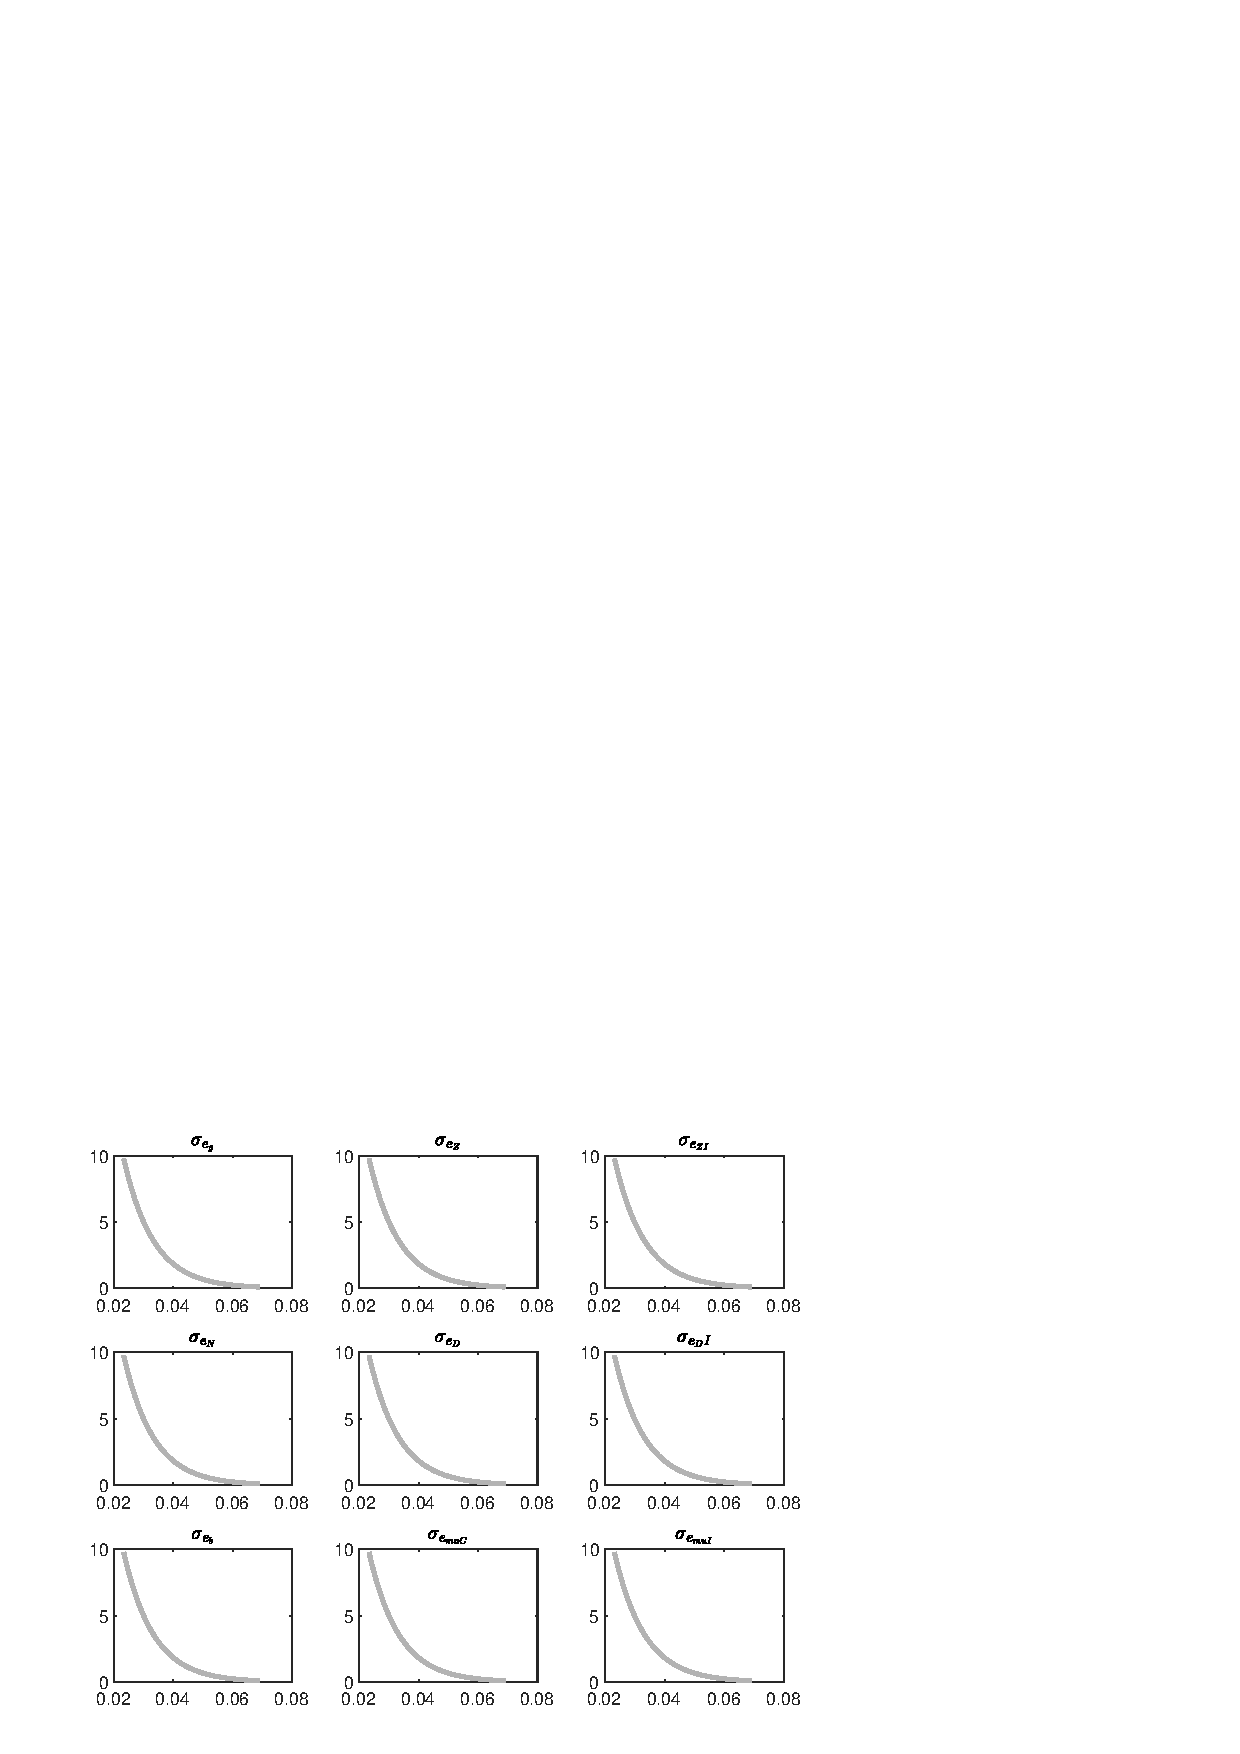
\includegraphics[width=0.80\textwidth]{BRS_sectoral_artificial_data/graphs/BRS_sectoral_artificial_data_Priors1}
\caption{Priors.}\label{Fig:Priors:1}
\end{figure}
\begin{figure}[H]
\centering
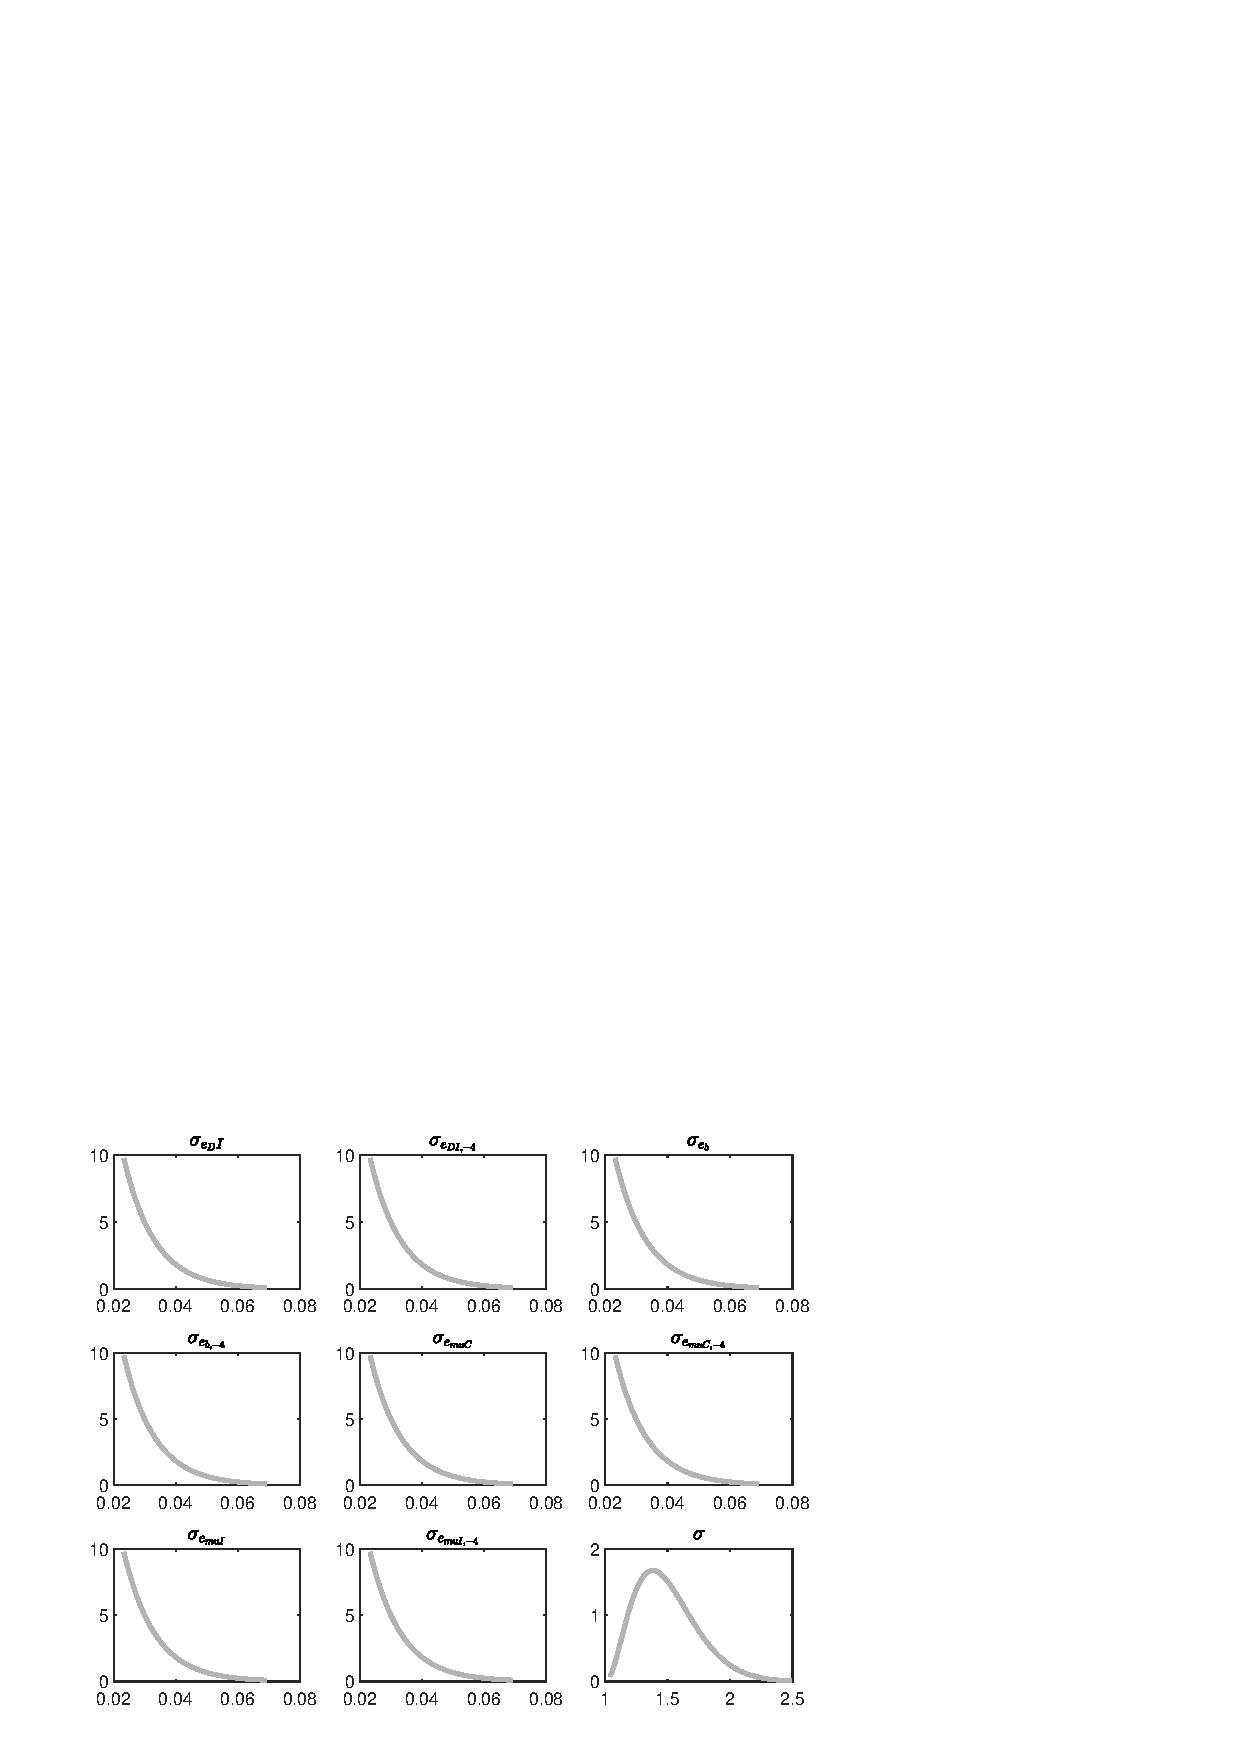
\includegraphics[width=0.80\textwidth]{BRS_sectoral_artificial_data/graphs/BRS_sectoral_artificial_data_Priors2}
\caption{Priors.}\label{Fig:Priors:2}
\end{figure}
\begin{figure}[H]
\centering
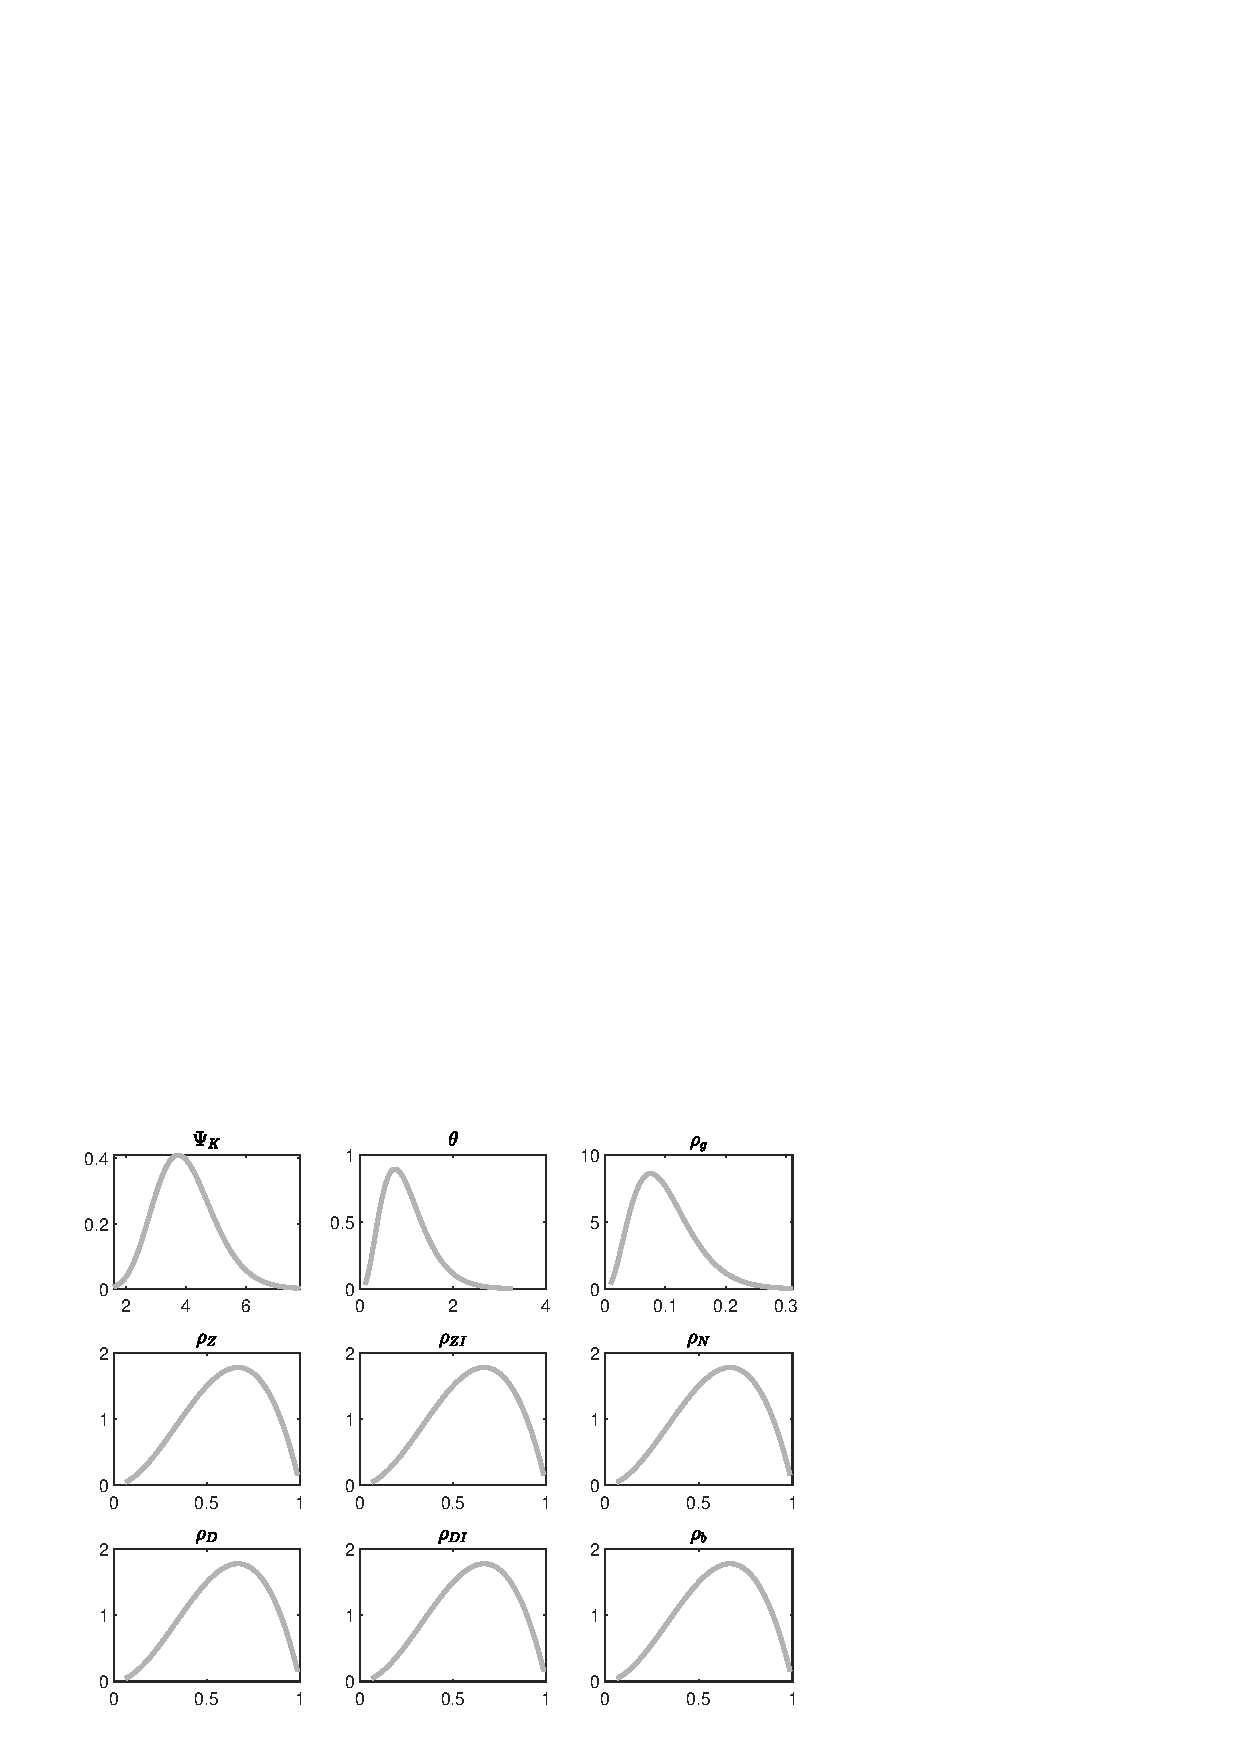
\includegraphics[width=0.80\textwidth]{BRS_sectoral_artificial_data/graphs/BRS_sectoral_artificial_data_Priors3}
\caption{Priors.}\label{Fig:Priors:3}
\end{figure}
\begin{figure}[H]
\centering
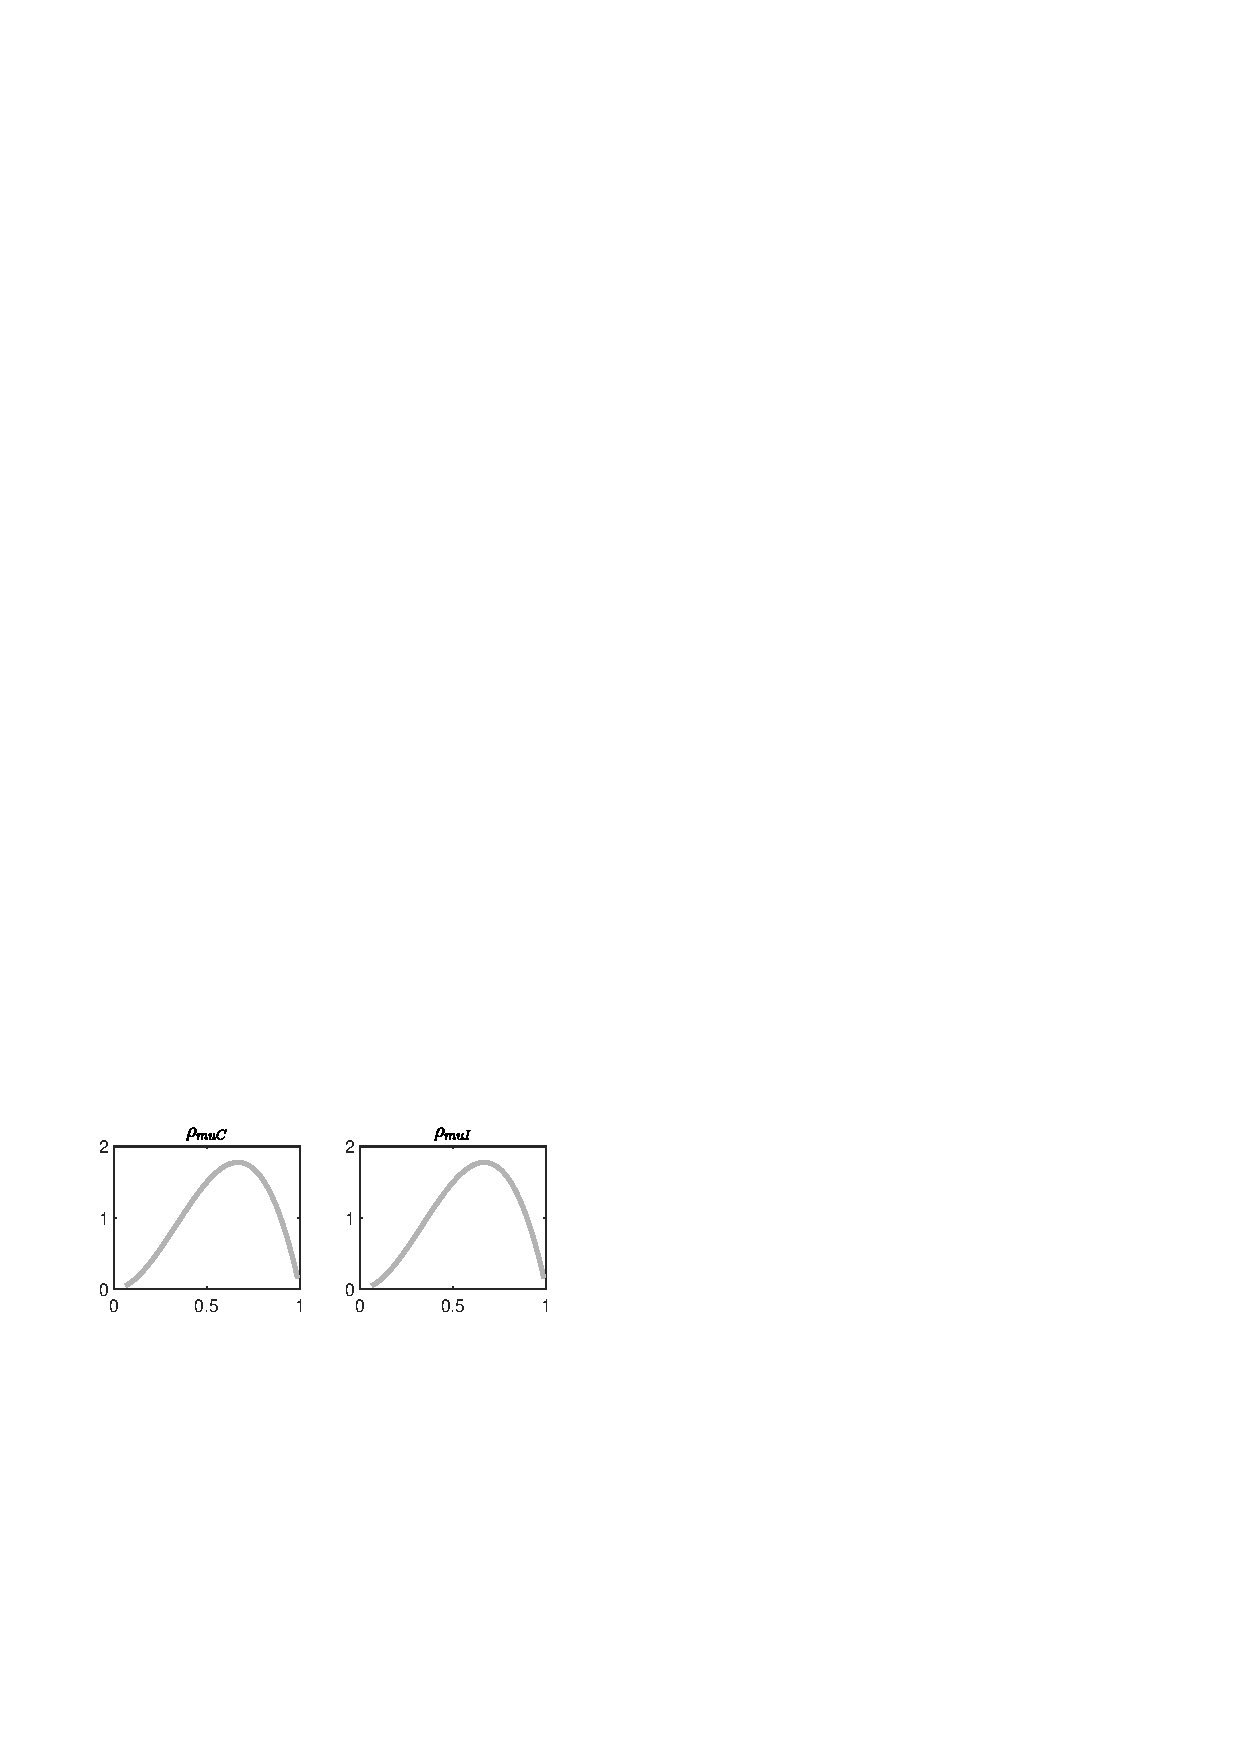
\includegraphics[width=0.53\textwidth]{BRS_sectoral_artificial_data/graphs/BRS_sectoral_artificial_data_Priors4}
\caption{Priors.}\label{Fig:Priors:4}
\end{figure}
 
% End of TeX file.
 
% TeX eps-loader file generated by PlotPosteriorDistributions.m (Dynare).
% 02-Oct-2024 10:39:42
 
\begin{figure}[H]
\centering
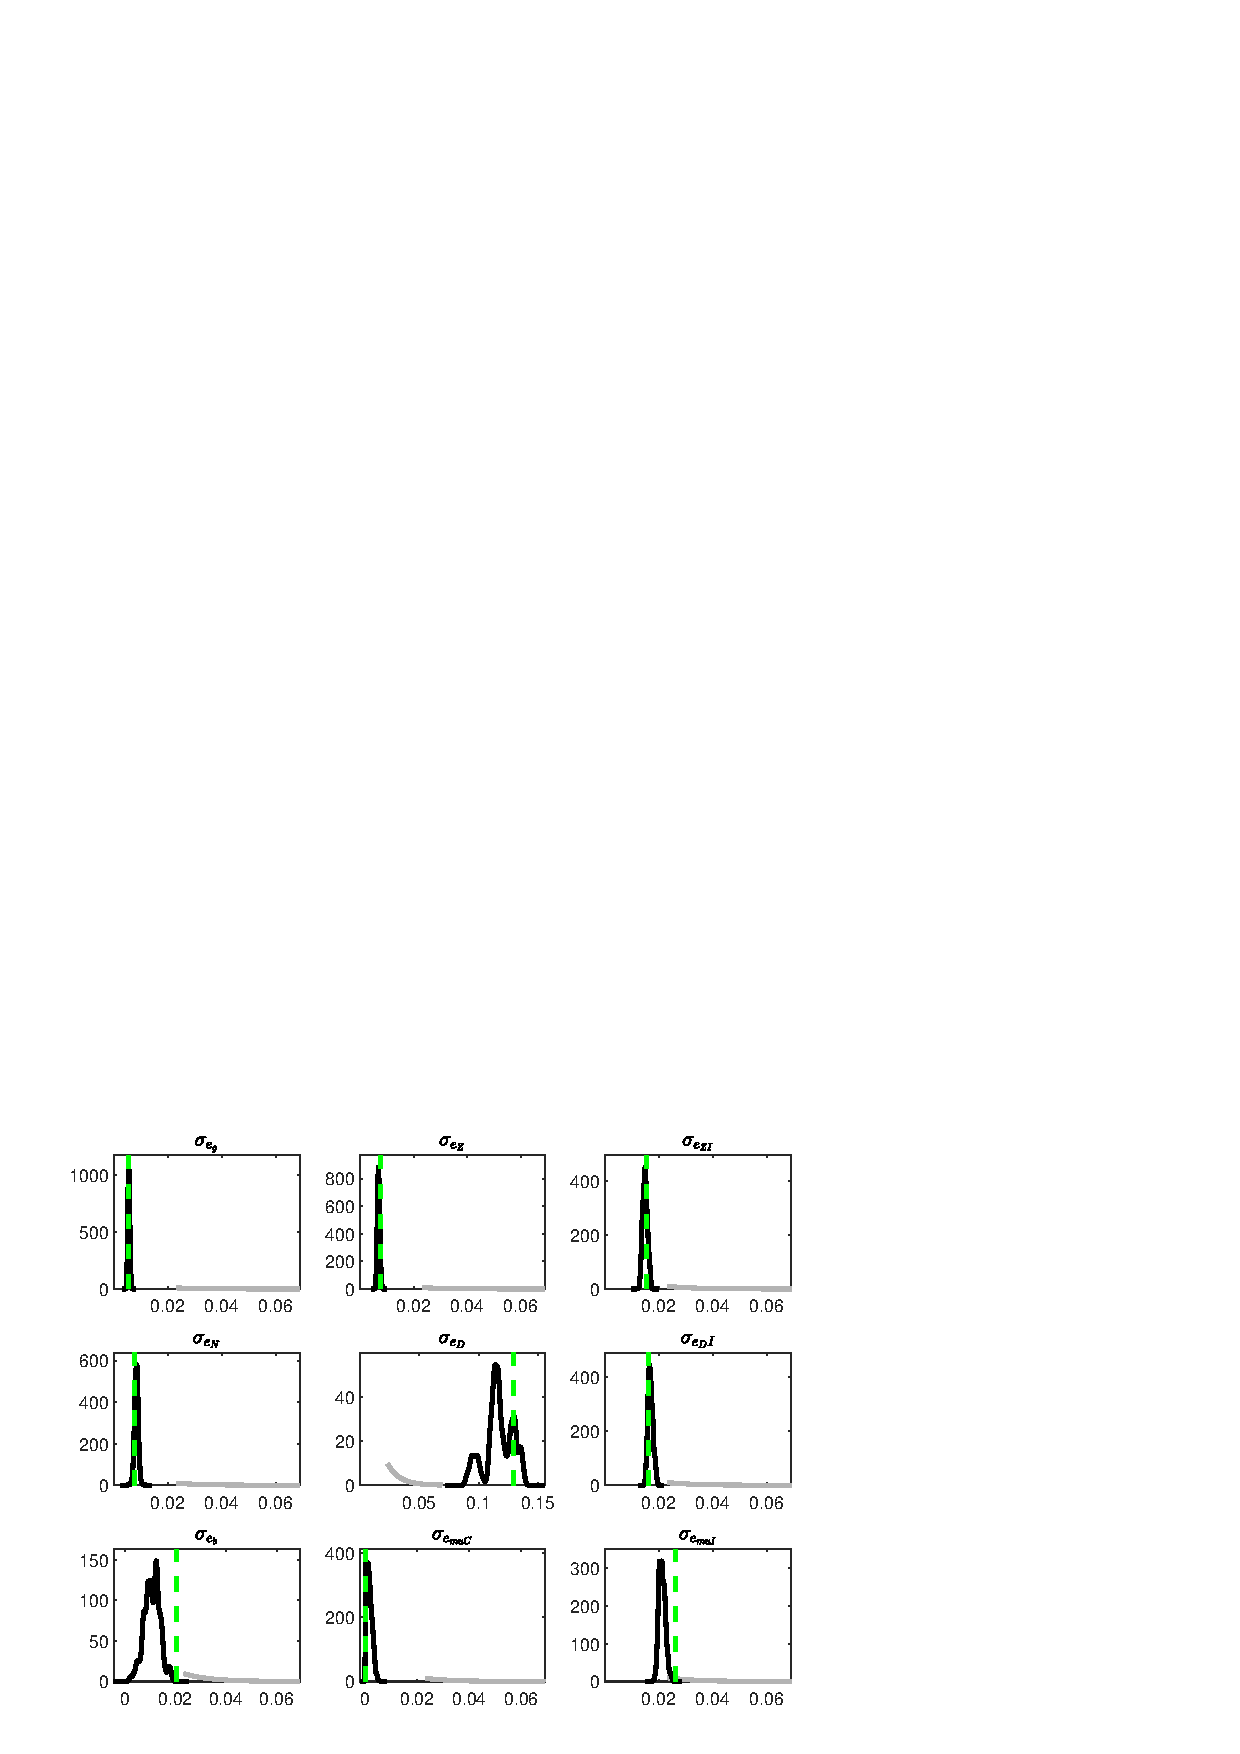
\includegraphics[width=0.80\textwidth]{BRS_sectoral_artificial_data/Output/BRS_sectoral_artificial_data_PriorsAndPosteriors1}
\caption{Priors and posteriors.}\label{Fig:PriorsAndPosteriors:1}
\end{figure}
 
\begin{figure}[H]
\centering
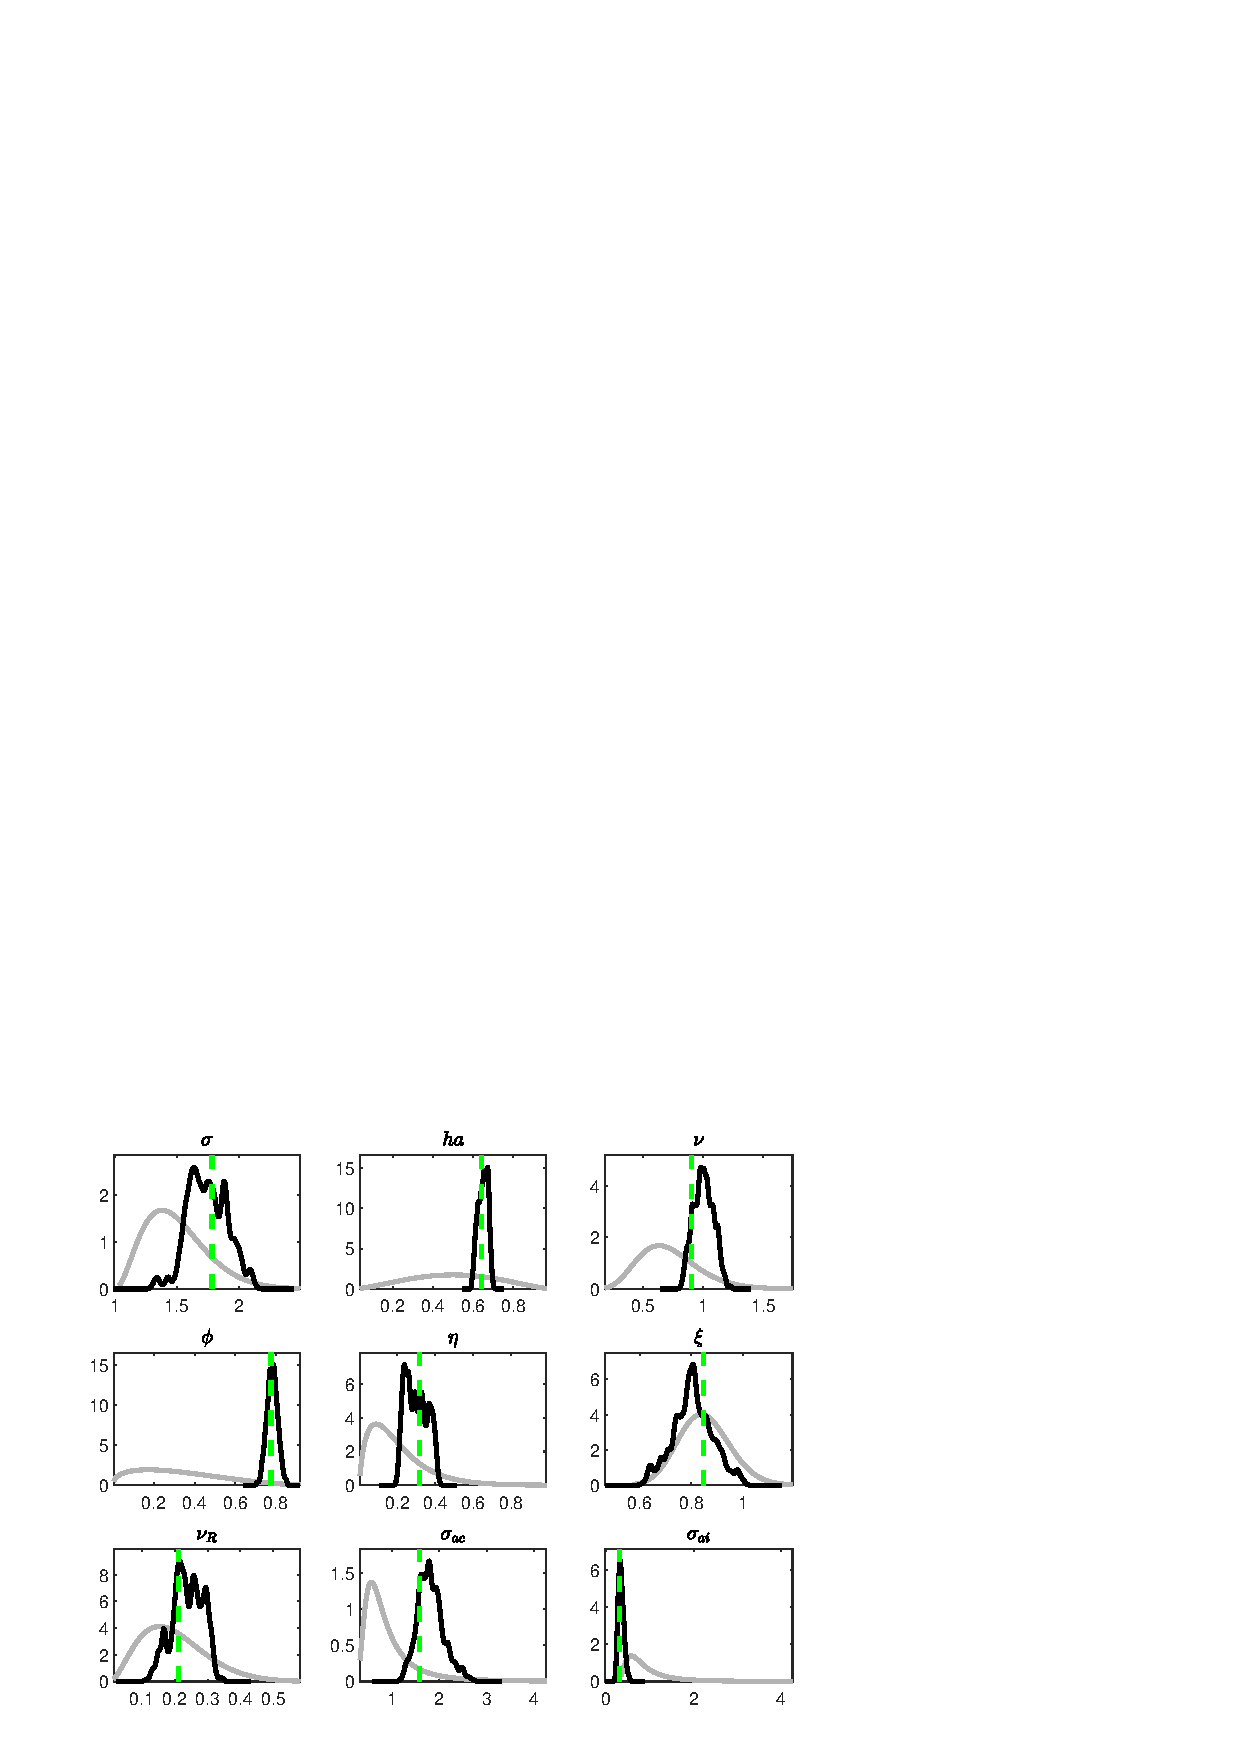
\includegraphics[width=0.80\textwidth]{BRS_sectoral_artificial_data/Output/BRS_sectoral_artificial_data_PriorsAndPosteriors2}
\caption{Priors and posteriors.}\label{Fig:PriorsAndPosteriors:2}
\end{figure}
 
\begin{figure}[H]
\centering
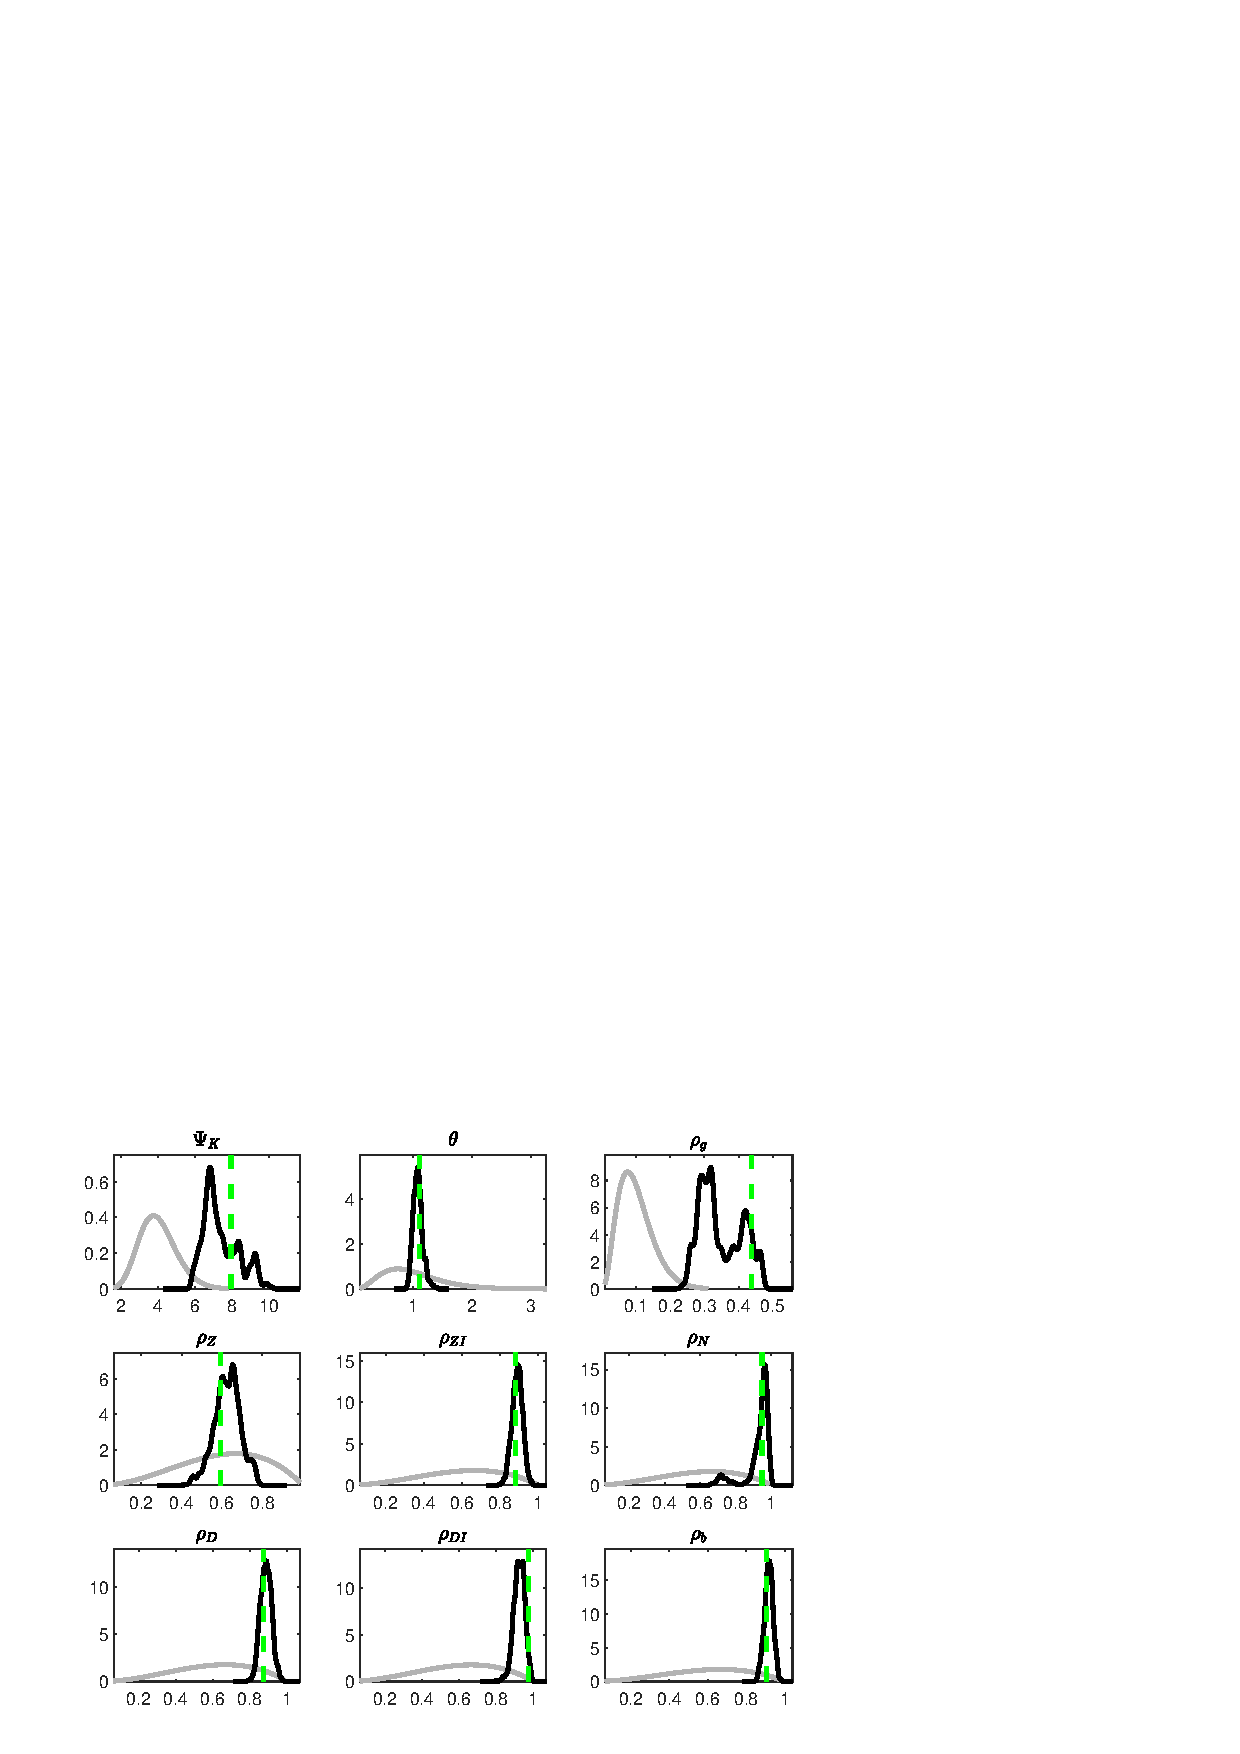
\includegraphics[width=0.80\textwidth]{BRS_sectoral_artificial_data/Output/BRS_sectoral_artificial_data_PriorsAndPosteriors3}
\caption{Priors and posteriors.}\label{Fig:PriorsAndPosteriors:3}
\end{figure}
 
\begin{figure}[H]
\centering
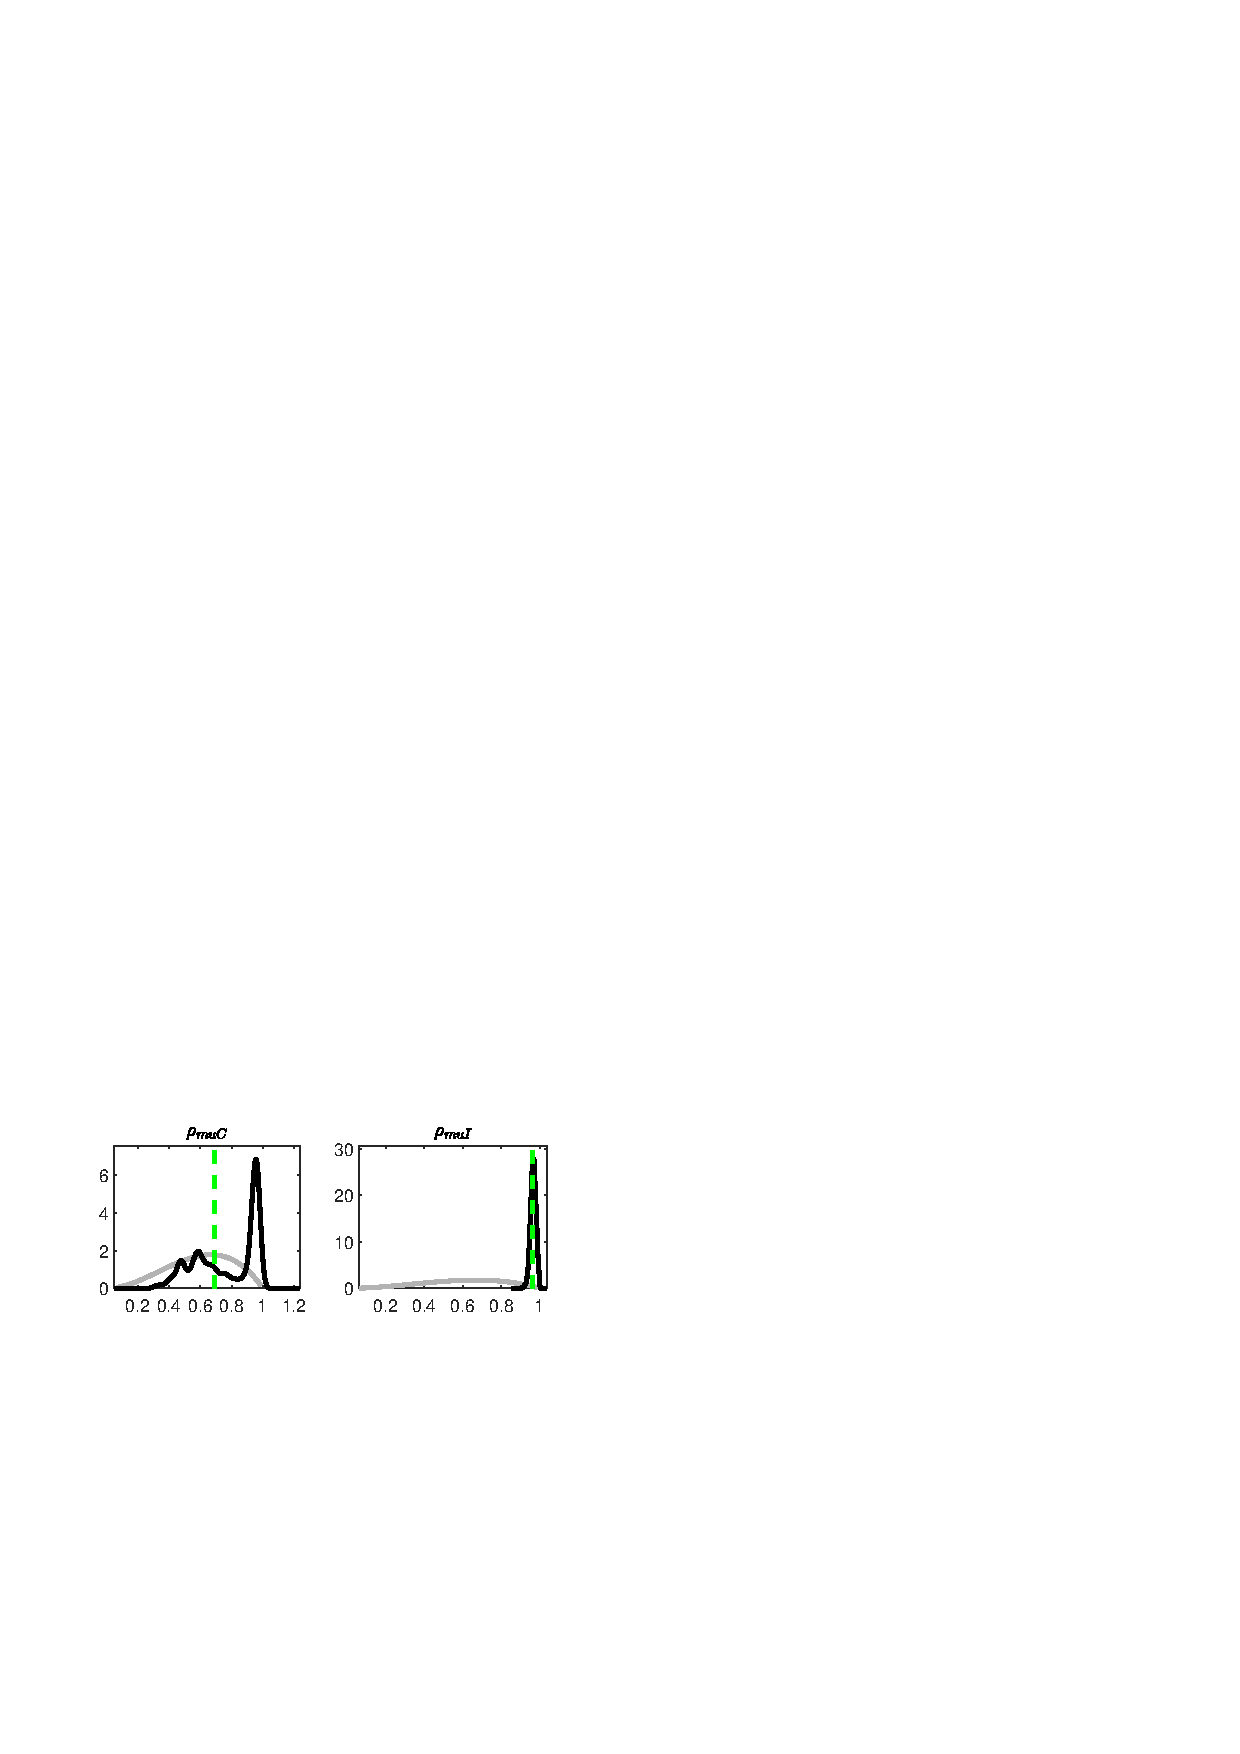
\includegraphics[width=0.53\textwidth]{BRS_sectoral_artificial_data/Output/BRS_sectoral_artificial_data_PriorsAndPosteriors4}
\caption{Priors and posteriors.}\label{Fig:PriorsAndPosteriors:4}
\end{figure}
 
% End of TeX file.
 
% TeX eps-loader file generated by mcmc_diagnostics.m (Dynare).
% 27-Jul-2025 17:52:36
 
\begin{figure}[H]
\centering 
\includegraphics[width=0.80\textwidth]{SU_sectoral_artificial_data/graphs/SU_sectoral_artificial_data_udiag1}
\caption{Univariate convergence diagnostics for the Metropolis-Hastings.
The first, second and third columns are respectively the criteria based on
the eighty percent interval, the second and third moments.}\label{Fig:UnivariateDiagnostics:1}
\end{figure}

\begin{figure}[H]
\centering 
\includegraphics[width=0.80\textwidth]{SU_sectoral_artificial_data/graphs/SU_sectoral_artificial_data_udiag2}
\caption{Univariate convergence diagnostics for the Metropolis-Hastings.
The first, second and third columns are respectively the criteria based on
the eighty percent interval, the second and third moments.}\label{Fig:UnivariateDiagnostics:2}
\end{figure}

\begin{figure}[H]
\centering 
\includegraphics[width=0.80\textwidth]{SU_sectoral_artificial_data/graphs/SU_sectoral_artificial_data_udiag3}
\caption{Univariate convergence diagnostics for the Metropolis-Hastings.
The first, second and third columns are respectively the criteria based on
the eighty percent interval, the second and third moments.}\label{Fig:UnivariateDiagnostics:3}
\end{figure}

\begin{figure}[H]
\centering 
\includegraphics[width=0.80\textwidth]{SU_sectoral_artificial_data/graphs/SU_sectoral_artificial_data_udiag4}
\caption{Univariate convergence diagnostics for the Metropolis-Hastings.
The first, second and third columns are respectively the criteria based on
the eighty percent interval, the second and third moments.}\label{Fig:UnivariateDiagnostics:4}
\end{figure}

\begin{figure}[H]
\centering 
\includegraphics[width=0.80\textwidth]{SU_sectoral_artificial_data/graphs/SU_sectoral_artificial_data_udiag5}
\caption{Univariate convergence diagnostics for the Metropolis-Hastings.
The first, second and third columns are respectively the criteria based on
the eighty percent interval, the second and third moments.}\label{Fig:UnivariateDiagnostics:5}
\end{figure}

\begin{figure}[H]
\centering 
\includegraphics[width=0.80\textwidth]{SU_sectoral_artificial_data/graphs/SU_sectoral_artificial_data_udiag6}
\caption{Univariate convergence diagnostics for the Metropolis-Hastings.
The first, second and third columns are respectively the criteria based on
the eighty percent interval, the second and third moments.}\label{Fig:UnivariateDiagnostics:6}
\end{figure}

\begin{figure}[H]
\centering 
\includegraphics[width=0.80\textwidth]{SU_sectoral_artificial_data/graphs/SU_sectoral_artificial_data_udiag7}
\caption{Univariate convergence diagnostics for the Metropolis-Hastings.
The first, second and third columns are respectively the criteria based on
the eighty percent interval, the second and third moments.}\label{Fig:UnivariateDiagnostics:7}
\end{figure}

\begin{figure}[H]
\centering 
\includegraphics[width=0.80\textwidth]{SU_sectoral_artificial_data/graphs/SU_sectoral_artificial_data_udiag8}
\caption{Univariate convergence diagnostics for the Metropolis-Hastings.
The first, second and third columns are respectively the criteria based on
the eighty percent interval, the second and third moments.}\label{Fig:UnivariateDiagnostics:8}
\end{figure}

\begin{figure}[H]
\centering 
\includegraphics[width=0.80\textwidth]{SU_sectoral_artificial_data/graphs/SU_sectoral_artificial_data_udiag9}
\caption{Univariate convergence diagnostics for the Metropolis-Hastings.
The first, second and third columns are respectively the criteria based on
the eighty percent interval, the second and third moments.}\label{Fig:UnivariateDiagnostics:9}
\end{figure}

\begin{figure}[H]
\centering 
\includegraphics[width=0.80\textwidth]{SU_sectoral_artificial_data/graphs/SU_sectoral_artificial_data_udiag10}
\caption{Univariate convergence diagnostics for the Metropolis-Hastings.
The first, second and third columns are respectively the criteria based on
the eighty percent interval, the second and third moments.}\label{Fig:UnivariateDiagnostics:10}
\end{figure}

% End Of TeX file. 
% 27-Jul-2025 17:55:19, created by stoch_simul.m 
 
\begin{center}
\begin{longtable}{lccccccccc} 
\caption{MATRIX OF COVARIANCE OF EXOGENOUS SHOCKS}\\
 \label{Table:covar_ex_shocks}\\
\toprule 
$Variables  $	 & 	 $        {e_g}$	 & 	 $        {e_Z}$	 & 	 $     {e_{ZI}}$	 & 	 $        {e_N}$	 & 	 $        {e_D}$	 & 	 $       {e_DI}$	 & 	 $        {e_b}$	 & 	 $    {e_{muC}}$	 & 	 $    {e_{muI}}$\\
\midrule \endfirsthead 
\caption{(continued)}\\
 \toprule \\ 
$Variables  $	 & 	 $        {e_g}$	 & 	 $        {e_Z}$	 & 	 $     {e_{ZI}}$	 & 	 $        {e_N}$	 & 	 $        {e_D}$	 & 	 $       {e_DI}$	 & 	 $        {e_b}$	 & 	 $    {e_{muC}}$	 & 	 $    {e_{muI}}$\\
\midrule \endhead 
\midrule \multicolumn{10}{r}{(Continued on next page)} \\ \bottomrule \endfoot 
\bottomrule \endlastfoot 
${e_g}      $	 & 	     0.000017	 & 	     0.000000	 & 	     0.000000	 & 	     0.000000	 & 	     0.000000	 & 	     0.000000	 & 	     0.000000	 & 	     0.000000	 & 	     0.000000 \\ 
${e_Z}      $	 & 	     0.000000	 & 	     0.000069	 & 	     0.000000	 & 	     0.000000	 & 	     0.000000	 & 	     0.000000	 & 	     0.000000	 & 	     0.000000	 & 	     0.000000 \\ 
${e_{ZI}}   $	 & 	     0.000000	 & 	     0.000000	 & 	     0.000343	 & 	     0.000000	 & 	     0.000000	 & 	     0.000000	 & 	     0.000000	 & 	     0.000000	 & 	     0.000000 \\ 
${e_N}      $	 & 	     0.000000	 & 	     0.000000	 & 	     0.000000	 & 	     0.000035	 & 	     0.000000	 & 	     0.000000	 & 	     0.000000	 & 	     0.000000	 & 	     0.000000 \\ 
${e_D}      $	 & 	     0.000000	 & 	     0.000000	 & 	     0.000000	 & 	     0.000000	 & 	     0.010430	 & 	     0.000000	 & 	     0.000000	 & 	     0.000000	 & 	     0.000000 \\ 
${e_DI}     $	 & 	     0.000000	 & 	     0.000000	 & 	     0.000000	 & 	     0.000000	 & 	     0.000000	 & 	     0.000211	 & 	     0.000000	 & 	     0.000000	 & 	     0.000000 \\ 
${e_b}      $	 & 	     0.000000	 & 	     0.000000	 & 	     0.000000	 & 	     0.000000	 & 	     0.000000	 & 	     0.000000	 & 	     0.000112	 & 	     0.000000	 & 	     0.000000 \\ 
${e_{muC}}  $	 & 	     0.000000	 & 	     0.000000	 & 	     0.000000	 & 	     0.000000	 & 	     0.000000	 & 	     0.000000	 & 	     0.000000	 & 	     0.000004	 & 	     0.000000 \\ 
${e_{muI}}  $	 & 	     0.000000	 & 	     0.000000	 & 	     0.000000	 & 	     0.000000	 & 	     0.000000	 & 	     0.000000	 & 	     0.000000	 & 	     0.000000	 & 	     0.000717 \\ 
\end{longtable}
 \end{center}
% End of TeX file.
 
% 27-Jul-2025 17:52:26, created by mcmc_diagnostics.m 
 
\begin{center}
\begin{longtable}{lcccccc} 
\caption{Geweke (1992) Convergence Tests, based on means of draws 120000 to 176000 vs 260000 to 400000 for chain 1. p-values are for $\chi^2$-test for equality of means.}\\
 \label{Table:geweke_block_1}\\
\toprule 
 & \multicolumn{2}{c}{Posterior} & \multicolumn{4}{c}{p-values} \\
\cmidrule(r{.75em}){2-3} \cmidrule(r{.75em}){4-7}
$Parameter             $	 & 	 $            Mean$	 & 	 $             Std$	 & 	 $      No\ Taper$	 & 	 $   4\%\ Taper$	 & 	 $   8\%\ Taper$	 & 	 $  15\%\ Taper$\\
\midrule \endfirsthead 
\caption{(continued)}\\
 \toprule \\ 
 & \multicolumn{2}{c}{Posterior} & \multicolumn{4}{c}{p-values} \\
\cmidrule(r{.75em}){2-3} \cmidrule(r{.75em}){4-7}
$Parameter             $	 & 	 $            Mean$	 & 	 $             Std$	 & 	 $      No\ Taper$	 & 	 $   4\%\ Taper$	 & 	 $   8\%\ Taper$	 & 	 $  15\%\ Taper$\\
\midrule \endhead 
\midrule \multicolumn{7}{r}{(Continued on next page)} \\ \bottomrule \endfoot 
\bottomrule \endlastfoot 
$ \sigma_{{e_g}}       $	 & 	          0.0041	 & 	          0.0003	 & 	          0.0000	 & 	          0.3666	 & 	          0.4299	 & 	          0.4497 \\ 
$ \sigma_{{e_Z}}       $	 & 	          0.0082	 & 	          0.0005	 & 	          0.0000	 & 	          0.1831	 & 	          0.2834	 & 	          0.3808 \\ 
$ \sigma_{{e_{ZI}}}    $	 & 	          0.0184	 & 	          0.0011	 & 	          0.0000	 & 	          0.0000	 & 	          0.0001	 & 	          0.0004 \\ 
$ \sigma_{{e_N}}       $	 & 	          0.0061	 & 	          0.0010	 & 	          0.0000	 & 	          0.0016	 & 	          0.0152	 & 	          0.0479 \\ 
$ \sigma_{{e_D}}       $	 & 	          0.1000	 & 	          0.0098	 & 	          0.0000	 & 	          0.0000	 & 	          0.0000	 & 	          0.0000 \\ 
$ \sigma_{{e_DI}}      $	 & 	          0.0144	 & 	          0.0008	 & 	          0.0000	 & 	          0.0615	 & 	          0.1102	 & 	          0.0901 \\ 
$ \sigma_{{e_b}}       $	 & 	          0.0111	 & 	          0.0032	 & 	          0.0000	 & 	          0.3011	 & 	          0.4429	 & 	          0.5446 \\ 
$ \sigma_{{e_{muC}}}   $	 & 	          0.0018	 & 	          0.0013	 & 	          0.0000	 & 	          0.8499	 & 	          0.8834	 & 	          0.9004 \\ 
$ \sigma_{{e_{muI}}}   $	 & 	          0.0271	 & 	          0.0015	 & 	          0.0000	 & 	          0.1237	 & 	          0.2080	 & 	          0.2687 \\ 
$ {\sigma}             $	 & 	          1.5791	 & 	          0.2115	 & 	          0.0000	 & 	          0.0000	 & 	          0.0000	 & 	          0.0000 \\ 
$ {ha}                 $	 & 	          0.7132	 & 	          0.0240	 & 	          0.0000	 & 	          0.0000	 & 	          0.0000	 & 	          0.0000 \\ 
$ \nu                  $	 & 	          1.2626	 & 	          0.1352	 & 	          0.0000	 & 	          0.0000	 & 	          0.0000	 & 	          0.0000 \\ 
$ {\phi}               $	 & 	          0.9088	 & 	          0.0256	 & 	          0.0000	 & 	          0.7479	 & 	          0.7789	 & 	          0.7809 \\ 
$ {\eta}               $	 & 	          0.2462	 & 	          0.0321	 & 	          0.0000	 & 	          0.0000	 & 	          0.0000	 & 	          0.0000 \\ 
$ \xi                  $	 & 	          0.7972	 & 	          0.0477	 & 	          0.0000	 & 	          0.0000	 & 	          0.0001	 & 	          0.0010 \\ 
$ {\nu_R}              $	 & 	          0.1370	 & 	          0.0406	 & 	          0.0000	 & 	          0.0000	 & 	          0.0001	 & 	          0.0029 \\ 
$ {\sigma_{ac}}        $	 & 	          2.0800	 & 	          0.2363	 & 	          0.0000	 & 	          0.6625	 & 	          0.7262	 & 	          0.7576 \\ 
$ {\sigma_{ai}}        $	 & 	          0.2963	 & 	          0.0508	 & 	          0.0000	 & 	          0.1226	 & 	          0.2149	 & 	          0.2693 \\ 
$ {\Psi_{K}}           $	 & 	          7.5692	 & 	          0.4736	 & 	          0.0000	 & 	          0.0000	 & 	          0.0000	 & 	          0.0001 \\ 
$ {\theta}             $	 & 	          1.5545	 & 	          0.1043	 & 	          0.0000	 & 	          0.2043	 & 	          0.3032	 & 	          0.3415 \\ 
$ {\rho_g}             $	 & 	          0.3357	 & 	          0.0260	 & 	          0.0000	 & 	          0.6696	 & 	          0.7518	 & 	          0.7983 \\ 
$ {\rho_Z}             $	 & 	          0.7115	 & 	          0.0715	 & 	          0.0000	 & 	          0.0003	 & 	          0.0059	 & 	          0.0221 \\ 
$ {\rho_{ZI}}          $	 & 	          0.8274	 & 	          0.0312	 & 	          0.0000	 & 	          0.0013	 & 	          0.0108	 & 	          0.0363 \\ 
$ {\rho_N}             $	 & 	          0.9245	 & 	          0.0392	 & 	          0.0000	 & 	          0.0430	 & 	          0.1190	 & 	          0.1879 \\ 
$ {\rho_D}             $	 & 	          0.8800	 & 	          0.0270	 & 	          0.0000	 & 	          0.7129	 & 	          0.7707	 & 	          0.8077 \\ 
$ {\rho_{DI}}          $	 & 	          0.9357	 & 	          0.0269	 & 	          0.0000	 & 	          0.0402	 & 	          0.1026	 & 	          0.1364 \\ 
$ {\rho_b}             $	 & 	          0.9156	 & 	          0.0253	 & 	          0.0000	 & 	          0.0535	 & 	          0.1420	 & 	          0.2310 \\ 
$ {\rho_{muC}}         $	 & 	          0.8840	 & 	          0.0708	 & 	          0.0000	 & 	          0.8948	 & 	          0.9174	 & 	          0.9286 \\ 
$ {\rho_{muI}}         $	 & 	          0.9603	 & 	          0.0156	 & 	          0.5822	 & 	          0.9877	 & 	          0.9884	 & 	          0.9870 \\ 
\end{longtable}
 \end{center}
% End of TeX file.
 
% 27-Jul-2025 17:52:36, created by mcmc_diagnostics.m 
 
\begin{center}
\begin{longtable}{lcccccc} 
\caption{Geweke (1992) Convergence Tests, based on means of draws 120000 to 176000 vs 260000 to 400000 for chain 2. p-values are for $\chi^2$-test for equality of means.}\\
 \label{Table:geweke_block_2}\\
\toprule 
 & \multicolumn{2}{c}{Posterior} & \multicolumn{4}{c}{p-values} \\
\cmidrule(r{.75em}){2-3} \cmidrule(r{.75em}){4-7}
$Parameter             $	 & 	 $            Mean$	 & 	 $             Std$	 & 	 $      No\ Taper$	 & 	 $   4\%\ Taper$	 & 	 $   8\%\ Taper$	 & 	 $  15\%\ Taper$\\
\midrule \endfirsthead 
\caption{(continued)}\\
 \toprule \\ 
 & \multicolumn{2}{c}{Posterior} & \multicolumn{4}{c}{p-values} \\
\cmidrule(r{.75em}){2-3} \cmidrule(r{.75em}){4-7}
$Parameter             $	 & 	 $            Mean$	 & 	 $             Std$	 & 	 $      No\ Taper$	 & 	 $   4\%\ Taper$	 & 	 $   8\%\ Taper$	 & 	 $  15\%\ Taper$\\
\midrule \endhead 
\midrule \multicolumn{7}{r}{(Continued on next page)} \\ \bottomrule \endfoot 
\bottomrule \endlastfoot 
$ \sigma_{{e_g}}       $	 & 	          0.0041	 & 	          0.0003	 & 	          0.0000	 & 	          0.3906	 & 	          0.3968	 & 	          0.3375 \\ 
$ \sigma_{{e_Z}}       $	 & 	          0.0082	 & 	          0.0006	 & 	          0.0000	 & 	          0.0002	 & 	          0.0025	 & 	          0.0141 \\ 
$ \sigma_{{e_{ZI}}}    $	 & 	          0.0183	 & 	          0.0012	 & 	          0.0000	 & 	          0.0000	 & 	          0.0000	 & 	          0.0001 \\ 
$ \sigma_{{e_N}}       $	 & 	          0.0060	 & 	          0.0007	 & 	          0.0000	 & 	          0.4356	 & 	          0.5123	 & 	          0.5360 \\ 
$ \sigma_{{e_D}}       $	 & 	          0.0957	 & 	          0.0073	 & 	          0.0000	 & 	          0.0000	 & 	          0.0011	 & 	          0.0092 \\ 
$ \sigma_{{e_DI}}      $	 & 	          0.0146	 & 	          0.0008	 & 	          0.0000	 & 	          0.1061	 & 	          0.1322	 & 	          0.1320 \\ 
$ \sigma_{{e_b}}       $	 & 	          0.0120	 & 	          0.0047	 & 	          0.0000	 & 	          0.5708	 & 	          0.6707	 & 	          0.7293 \\ 
$ \sigma_{{e_{muC}}}   $	 & 	          0.0018	 & 	          0.0011	 & 	          0.0000	 & 	          0.0703	 & 	          0.1223	 & 	          0.1358 \\ 
$ \sigma_{{e_{muI}}}   $	 & 	          0.0265	 & 	          0.0018	 & 	          0.0000	 & 	          0.0182	 & 	          0.0508	 & 	          0.0667 \\ 
$ {\sigma}             $	 & 	          1.7733	 & 	          0.1207	 & 	          0.0000	 & 	          0.4217	 & 	          0.5495	 & 	          0.6332 \\ 
$ {ha}                 $	 & 	          0.6996	 & 	          0.0168	 & 	          0.0000	 & 	          0.0073	 & 	          0.0448	 & 	          0.1164 \\ 
$ \nu                  $	 & 	          1.2747	 & 	          0.1123	 & 	          0.0000	 & 	          0.0000	 & 	          0.0000	 & 	          0.0008 \\ 
$ {\phi}               $	 & 	          0.9090	 & 	          0.0276	 & 	          0.0000	 & 	          0.1973	 & 	          0.3041	 & 	          0.3804 \\ 
$ {\eta}               $	 & 	          0.2623	 & 	          0.0264	 & 	          0.0000	 & 	          0.0019	 & 	          0.0209	 & 	          0.0705 \\ 
$ \xi                  $	 & 	          0.8048	 & 	          0.0542	 & 	          0.0000	 & 	          0.0000	 & 	          0.0000	 & 	          0.0000 \\ 
$ {\nu_R}              $	 & 	          0.1349	 & 	          0.0507	 & 	          0.0000	 & 	          0.0006	 & 	          0.0128	 & 	          0.0562 \\ 
$ {\sigma_{ac}}        $	 & 	          1.9922	 & 	          0.2135	 & 	          0.0000	 & 	          0.6234	 & 	          0.7030	 & 	          0.7446 \\ 
$ {\sigma_{ai}}        $	 & 	          0.2908	 & 	          0.0468	 & 	          0.0000	 & 	          0.0626	 & 	          0.1240	 & 	          0.1914 \\ 
$ {\Psi_{K}}           $	 & 	          7.8211	 & 	          0.4412	 & 	          0.0000	 & 	          0.0018	 & 	          0.0211	 & 	          0.0714 \\ 
$ {\theta}             $	 & 	          1.5302	 & 	          0.1054	 & 	          0.0000	 & 	          0.0000	 & 	          0.0003	 & 	          0.0014 \\ 
$ {\rho_g}             $	 & 	          0.2982	 & 	          0.0527	 & 	          0.0000	 & 	          0.0000	 & 	          0.0000	 & 	          0.0000 \\ 
$ {\rho_Z}             $	 & 	          0.7442	 & 	          0.0459	 & 	          0.0000	 & 	          0.6510	 & 	          0.7107	 & 	          0.7254 \\ 
$ {\rho_{ZI}}          $	 & 	          0.8199	 & 	          0.0301	 & 	          0.0000	 & 	          0.7425	 & 	          0.7820	 & 	          0.8007 \\ 
$ {\rho_N}             $	 & 	          0.9223	 & 	          0.0362	 & 	          0.0000	 & 	          0.0260	 & 	          0.0873	 & 	          0.1600 \\ 
$ {\rho_D}             $	 & 	          0.8845	 & 	          0.0265	 & 	          0.0000	 & 	          0.2589	 & 	          0.3747	 & 	          0.4594 \\ 
$ {\rho_{DI}}          $	 & 	          0.9238	 & 	          0.0333	 & 	          0.0000	 & 	          0.0051	 & 	          0.0280	 & 	          0.0669 \\ 
$ {\rho_b}             $	 & 	          0.9190	 & 	          0.0240	 & 	          0.0000	 & 	          0.3824	 & 	          0.5132	 & 	          0.6010 \\ 
$ {\rho_{muC}}         $	 & 	          0.8839	 & 	          0.0918	 & 	          0.0000	 & 	          0.0478	 & 	          0.1273	 & 	          0.1998 \\ 
$ {\rho_{muI}}         $	 & 	          0.9606	 & 	          0.0161	 & 	          0.0000	 & 	          0.1390	 & 	          0.1705	 & 	          0.1497 \\ 
\end{longtable}
 \end{center}
% End of TeX file.
 
\begin{center}
\begin{longtable}{ccc}
\caption{Endogenous}\\%
\hline%
\multicolumn{1}{c}{\textbf{Variable}} &
\multicolumn{1}{c}{\textbf{\LaTeX}} &
\multicolumn{1}{c}{\textbf{Description}}\\%
\hline\hline%
\endfirsthead
\multicolumn{3}{c}{{\tablename} \thetable{} -- Continued}\\%
\hline%
\multicolumn{1}{c}{\textbf{Variable}} &
\multicolumn{1}{c}{\textbf{\LaTeX}} &
\multicolumn{1}{c}{\textbf{Description}}\\%
\hline\hline%
\endhead
\texttt{Y} & ${Y}$ & output\\
\texttt{C} & ${C}$ & consumption\\
\texttt{Y\_mc} & ${Y_{mc}}$ & consumption non-durable goods\\
\texttt{Y\_sc} & $Y_{sc}}$ & consumption services\\
\texttt{SR} & ${SR}$ & aggregate share-weighted Solow residual\\
\texttt{I} & ${I}$ & investment\\
\texttt{I\_mc} & ${I_C}$ & investment:mc\\
\texttt{I\_sc} & ${I_C}$ & investment:sc\\
\texttt{I\_I} & ${I_I}$ & investment:I\\
\texttt{K} & ${K}$ & Capital\\
\texttt{K\_mc} & ${K_{mc}}$ & Capital:mc\\
\texttt{K\_sc} & ${K_{sc}}$ & Capital:sc\\
\texttt{K\_I} & ${K_I}$ & Capital:I\\
\texttt{N} & ${N}$ & Hours\\
\texttt{N\_mc} & ${N_{mc}}$ & Hours:mc\\
\texttt{N\_sc} & ${N_{sc}}$ & Hours:sc\\
\texttt{N\_C} & ${N_C}$ & Hours:C\\
\texttt{N\_I} & ${N_I}$ & Hours:I\\
\texttt{N\_comp} & ${N}$ & Labor CES aggregate\\
\texttt{Z\_C} & ${Z_{C}}$ & Tech:mc\\
\texttt{u\_ZI} & $u\_ZI$ & u\_ZI\\
\texttt{Z\_I} & ${Z_I}$ & Tech:I\\
\texttt{tech} & ${tech}$ & General technology measure\\
\texttt{theta\_N} & ${\theta_N}$ & Labor disutility\\
\texttt{theta\_D} & ${\theta_D}$ & Shopping disutility\\
\texttt{theta\_I} & ${\theta_I}$ & Relative shopping disutility\\
\texttt{theta\_b} & ${\theta_b}$ & Discount factor shock\\
\texttt{mu\_C} & ${\mu_C}$ & mu\_C\\
\texttt{mu\_I} & $\mu_I}$ & mu\_I\\
\texttt{R\_mc} & ${R_{mc}}$ & Capital rental rate:mc\\
\texttt{R\_sc} & ${R_{sc}}$ & Capital rental rate:sc\\
\texttt{R\_I} & ${R_I}$ & Capital rental rate:I\\
\texttt{W\_C} & ${W_C}$ & Real wage:C\\
\texttt{W\_I} & ${W_I}$ & Real wage:I\\
\texttt{W} & ${W}$ & Real wage\\
\texttt{h\_mc} & ${h_mc}$ & Capital utilization rate:mc\\
\texttt{h\_sc} & ${h_sc}$ & Capital utilization rate:sc\\
\texttt{h\_I} & ${h_I}$ & Capital utilization rate:I\\
\texttt{h} & $h$ & Capital utilization rate: average\\
\texttt{delta\_mc} & ${\delta_{mc}}$ & Capital depreciation rate:mc\\
\texttt{delta\_sc} & ${\delta_{sc}}$ & Capital depreciation rate:sc\\
\texttt{delta\_I} & ${\delta_I}$ & Capital depreciation rate:I\\
\texttt{delta\_mc\_pr} & ${\delta_{mc,pr}$ & Capital depreciation rate derivative:mc\\
\texttt{delta\_sc\_pr} & ${\delta_{sc,pr}}$ & Capital depreciation rate derivative:sc\\
\texttt{delta\_I\_pr} & ${\delta_{I,pr}}$ & Capital depreciation rate derivative:I\\
\texttt{Smc} & $S$ & Investment adjustment cost:mc\\
\texttt{Ssc} & $S$ & Investment adjustment cost:sc\\
\texttt{Si} & $S$ & Investment adjustment cost:I\\
\texttt{Smc\_pr} & $S_pr$ & Derivative investment adjustment cost:mc\\
\texttt{Ssc\_pr} & $S_pr$ & Derivative investment adjustment cost:sc\\
\texttt{Si\_pr} & $S_pr$ & Derivative investment adjustment cost:I\\
\texttt{D} & ${D}$ & Shopping effort\\
\texttt{D\_mc} & ${D_{mc}}$ & Shopping effort:mc\\
\texttt{D\_sc} & ${D_{sc}}$ & Shopping effort:sc\\
\texttt{D\_I} & ${D_I}$ & Shopping effort:I\\
\texttt{Gam} & ${\Gamma}$ & Composite utility term\\
\texttt{p\_mc} & ${p_{mc}}$ & Relative non-durable price\\
\texttt{p\_sc} & ${p_{sc}}$ & Relative service price\\
\texttt{p\_I} & ${p_I}$ & Relative investment price\\
\texttt{lam} & ${\lambda}$ & Marginal utility of wealth\\
\texttt{Q\_mc} & ${Q}$ & Relative price of capital:mc\\
\texttt{Q\_sc} & ${Q}$ & Relative price of capital:sc\\
\texttt{Q\_I} & ${Q}$ & Relative price of capital:I\\
\texttt{x\_mc} & ${x}$ & Growth rate of investment:mc\\
\texttt{x\_sc} & ${x}$ & Growth rate of investment:sc\\
\texttt{x\_I} & ${x}$ & Growth rate of investment:I\\
\texttt{log\_SR} & $log\_SR$ & Solow residual\\
\texttt{util} & ${util}$ & Capacity utilization\\
\texttt{util\_ND} & ${util_{ND}}$ & Capacity utilization:ND\\
\texttt{util\_sc} & ${util_{sc}}$ & Capacity utilization:sc\\
\texttt{util\_D} & ${util_D}$ & Capacity utilization:D\\
\texttt{g} & ${g}$ & Growth rate of stochastic trend\\
\texttt{log\_Y} & $log\_Y$ & log\_Y\\
\texttt{log\_C} & $log\_C$ & log\_C\\
\texttt{log\_I} & $log\_I$ & log\_I\\
\texttt{log\_N} & $log\_N$ & log\_N\\
\texttt{log\_NC} & $log\_NC$ & log\_NC\\
\texttt{log\_NI} & $log\_NI$ & log\_NI\\
\texttt{log\_K} & $log\_K$ & log\_K\\
\texttt{log\_Y\_N} & $log\_Y\_N$ & log\_Y\_N\\
\texttt{log\_D} & $log\_D$ & log\_D\\
\texttt{log\_h} & $log\_h$ & log\_h\\
\texttt{log\_p\_I} & $log\_p\_I$ & log\_p\_I\\
\texttt{log\_util} & $log\_util$ & log\_util\\
\texttt{log\_util\_ND} & $log\_util\_ND$ & log\_util\_ND\\
\texttt{log\_util\_D} & $log\_util\_D$ & log\_util\_D\\
\texttt{log\_W} & $log\_W$ & log\_W\\
\texttt{log\_tech} & $log\_tech$ & log\_tech\\
\texttt{C\_obs} & $C\_obs$ & C\_obs\\
\texttt{I\_obs} & $I\_obs$ & I\_obs\\
\texttt{Y\_obs} & $Y\_obs$ & Y\_obs\\
\texttt{SR\_obs} & $SR\_obs$ & SR\_obs\\
\texttt{Y\_N\_obs} & $Y\_N\_obs$ & Y\_N\_obs\\
\texttt{p\_I\_obs} & $p\_I\_obs$ & p\_I\_obs\\
\texttt{N\_obs} & $N\_obs$ & N\_obs\\
\texttt{NC\_obs} & $NC\_obs$ & NC\_obs\\
\texttt{NI\_obs} & $NI\_obs$ & NI\_obs\\
\texttt{util\_ND\_obs} & $util\_ND\_obs$ & util\_ND\_obs\\
\texttt{util\_D\_obs} & $util\_D\_obs$ & util\_D\_obs\\
\texttt{util\_obs} & $util\_obs$ & util\_obs\\
\texttt{tech\_obs} & $tech\_obs$ & tech\_obs\\
\texttt{w\_obs} & $w\_obs$ & w\_obs\\
\texttt{D\_obs} & $D\_obs$ & D\_obs\\
\texttt{h\_obs} & $h\_obs$ & h\_obs\\
\texttt{K\_obs} & $K\_obs$ & K\_obs\\
\hline%
\end{longtable}
\end{center}
\begin{center}
\begin{longtable}{ccc}
\caption{Exogenous}\\%
\hline%
\multicolumn{1}{c}{\textbf{Variable}} &
\multicolumn{1}{c}{\textbf{\LaTeX}} &
\multicolumn{1}{c}{\textbf{Description}}\\%
\hline\hline%
\endfirsthead
\multicolumn{3}{c}{{\tablename} \thetable{} -- Continued}\\%
\hline%
\multicolumn{1}{c}{\textbf{Variable}} &
\multicolumn{1}{c}{\textbf{\LaTeX}} &
\multicolumn{1}{c}{\textbf{Description}}\\%
\hline\hline%
\endhead
\texttt{e\_g} & ${e_g}$ & Labor-augmenting-technology growth shock\\
\texttt{e\_Z} & ${e_Z}$ & TFP shock\\
\texttt{e\_ZI} & ${e_{ZI}}$ & Investment-specific tech shock\\
\texttt{e\_N} & ${e_N}$ & Labor supply shock\\
\texttt{e\_D} & ${e_D}$ & Shopping disutility shock\\
\texttt{e\_DI} & ${e_DI}$ & Relative investment shopping disutility shock\\
\texttt{e\_b} & ${e_b}$ & Discount factor shock\\
\texttt{e\_muC} & ${e_{muC}}$ & Wage markup shock: C\\
\texttt{e\_muI} & ${e_{muI}}$ & Wage markup shock: I\\
\hline%
\end{longtable}
\end{center}
\begin{center}
\begin{longtable}{ccc}
\caption{Parameters}\\%
\hline%
\multicolumn{1}{c}{\textbf{Variable}} &
\multicolumn{1}{c}{\textbf{\LaTeX}} &
\multicolumn{1}{c}{\textbf{Description}}\\%
\hline\hline%
\endfirsthead
\multicolumn{3}{c}{{\tablename} \thetable{} -- Continued}\\%
\hline%
\multicolumn{1}{c}{\textbf{Variable}} &
\multicolumn{1}{c}{\textbf{\LaTeX}} &
\multicolumn{1}{c}{\textbf{Description}}\\%
\hline\hline%
\endhead
\texttt{sigma} & ${\sigma}$ & Risk aversion\\
\texttt{beta} & ${\beta}$ & Discount factor\\
\texttt{g\_bar} & ${\overline{g}}$ & Quarterly trend growth rate\\
\texttt{nu} & $\nu$ & Frisch elasticity\\
\texttt{xi} & $\xi$ & elasticity of substitution between non-durables and services\\
\texttt{omega\_sc} & $\omega_{sc}$ & Weight of services in aggregator\\
\texttt{mu\_ss} & $\mu_{ss}$ & steady-state wage markup\\
\texttt{sigma\_ac} & ${\sigma_{ac}}$ & Inverse elasticity of marginal utilization cost wrt rental rate:C\\
\texttt{sigma\_ai} & ${\sigma_{ai}}$ & Inverse elasticity of marginal utilization cost wrt rental rate:I\\
\texttt{Psi\_K} & ${\Psi_{K}}$ & Investment adjustment cost parameter\\
\texttt{I\_Y} & ${I_Y}$ & Investment-output ratio\\
\texttt{K\_Y} & ${K_Y}$ & Capital-output ratio (quarterly)\\
\texttt{labor\_share} & $(labor share)$ & Labor share\\
\texttt{nu\_R} & ${\nu_R}$ & Fixed cost share\\
\texttt{ha} & ${ha}$ & Habit persistence\\
\texttt{phi} & ${\phi}$ & Shopping matching function elasticity\\
\texttt{eta} & ${\eta}$ & Shopping disutility\\
\texttt{Psi} & ${\Psi}$ & Matching utilization\\
\texttt{theta} & ${\theta}$ & Inverse intersectoral elasticity of labor supply\\
\texttt{rho\_g} & ${\rho_g}$ & persistence TFP growth shock\\
\texttt{rho\_Z} & ${\rho_Z}$ & persistence TFP shock\\
\texttt{rho\_ZI} & ${\rho_{ZI}}$ & persistence I-specific shock\\
\texttt{rho\_N} & ${\rho_N}$ & persistence labor supply shock\\
\texttt{rho\_D} & ${\rho_D}$ & persistence shopping effort shock\\
\texttt{rho\_DI} & ${\rho_{DI}}$ & persistence relative shopping effort shock\\
\texttt{rho\_b} & ${\rho_b}$ & persistence discount factor shock\\
\texttt{rho\_muC} & ${\rho_{muC}}$ & persistence wage markup shock:C\\
\texttt{rho\_muI} & ${\rho_{muI}}$ & persistence wage markup shock:I\\
\texttt{p\_I\_ss} & $p\_I\_ss$ & p\_I\_ss\\
\texttt{N\_ss} & $N\_ss$ & N\_ss\\
\hline%
\end{longtable}
\end{center}
 
\begin{center}
\begin{longtable}{ccc}
\caption{Parameter Values}\\%
\toprule%
\multicolumn{1}{c}{\textbf{Parameter}} &
\multicolumn{1}{c}{\textbf{Value}} &
 \multicolumn{1}{c}{\textbf{Description}}\\%
\midrule%
\endfirsthead
\multicolumn{3}{c}{{\tablename} \thetable{} -- Continued}\\%
\midrule%
\multicolumn{1}{c}{\textbf{Parameter}} &
\multicolumn{1}{c}{\textbf{Value}} &
  \multicolumn{1}{c}{\textbf{Description}}\\%
\midrule%
\endhead
${\sigma}$ 	 & 	 1.631 	 & 	 Risk aversion\\
${\beta}$ 	 & 	 0.990 	 & 	 Discount factor\\
${\overline{g}}$ 	 & 	 0.004 	 & 	 Quarterly trend growth rate\\
$\nu$ 	 & 	 1.296 	 & 	 Frisch elasticity\\
$\xi$ 	 & 	 0.804 	 & 	 elasticity of substitution between non-durables and services\\
$\omega_{sc}$ 	 & 	 0.650 	 & 	 Weight of services in aggregator\\
$\mu_{ss}$ 	 & 	 1.150 	 & 	 steady-state wage markup\\
${\sigma_{ac}}$ 	 & 	 2.059 	 & 	 Inverse elasticity of marginal utilization cost wrt rental rate:C\\
${\sigma_{ai}}$ 	 & 	 0.296 	 & 	 Inverse elasticity of marginal utilization cost wrt rental rate:I\\
${\Psi_{K}}$ 	 & 	 7.785 	 & 	 Investment adjustment cost parameter\\
${I_Y}$ 	 & 	 0.200 	 & 	 Investment-output ratio\\
${K_Y}$ 	 & 	 11.000 	 & 	 Capital-output ratio (quarterly)\\
$(labor share)$ 	 & 	 0.670 	 & 	 Labor share\\
${\nu_R}$ 	 & 	 0.127 	 & 	 Fixed cost share\\
${ha}$ 	 & 	 0.715 	 & 	 Habit persistence\\
${\phi}$ 	 & 	 0.912 	 & 	 Shopping matching function elasticity\\
${\eta}$ 	 & 	 0.241 	 & 	 Shopping disutility\\
${\Psi}$ 	 & 	 0.810 	 & 	 Matching utilization\\
${\theta}$ 	 & 	 1.538 	 & 	 Inverse intersectoral elasticity of labor supply\\
${\rho_g}$ 	 & 	 0.316 	 & 	 persistence TFP growth shock\\
${\rho_Z}$ 	 & 	 0.740 	 & 	 persistence TFP shock\\
${\rho_{ZI}}$ 	 & 	 0.820 	 & 	 persistence I-specific shock\\
${\rho_N}$ 	 & 	 0.911 	 & 	 persistence labor supply shock\\
${\rho_D}$ 	 & 	 0.885 	 & 	 persistence shopping effort shock\\
${\rho_{DI}}$ 	 & 	 0.930 	 & 	 persistence relative shopping effort shock\\
${\rho_b}$ 	 & 	 0.918 	 & 	 persistence discount factor shock\\
${\rho_{muC}}$ 	 & 	 0.916 	 & 	 persistence wage markup shock:C\\
${\rho_{muI}}$ 	 & 	 0.959 	 & 	 persistence wage markup shock:I\\
$p\_I\_ss$ 	 & 	 1.000 	 & 	 p\_I\_ss\\
$N\_ss$ 	 & 	 0.300 	 & 	 N\_ss\\
\bottomrule%
\end{longtable}
\end{center}
 
% TeX-table generated by Dynare write_latex_prior_table.m.
% Prior Information
% 27-Jul-2025 17:55:17 
 
\begin{center}
\begin{longtable}{lcccccccc} 
\caption{Prior information (parameters)}\\
 \label{Table:Prior}\\
\toprule%
  &  &  &  &  & \multicolumn{2}{c}{Bounds} & \multicolumn{2}{c}{90\% HPDI} \\ 
  \cmidrule(r{.75em}){6-7} \cmidrule(r{.75em}){8-9}
  & Distribution & Mean & Mode & Std.dev. & Lower & Upper & Lower & Upper  \\ 
\midrule
\endfirsthead
\caption{(continued)}\\
 \toprule%
  &  &  &  &  & \multicolumn{2}{c}{Bounds} & \multicolumn{2}{c}{90\% HPDI} \\ 
  \cmidrule(r{.75em}){6-7} \cmidrule(r{.75em}){8-9}
  & Distribution & Mean & Mode & Std.dev. & Lower & Upper & Lower & Upper  \\ 
\midrule
\endhead
\midrule
\multicolumn{9}{r}{(Continued on next page)} \\ 
\bottomrule
\endfoot
\bottomrule
\endlastfoot
$ \sigma_{{e_g}} $ & Gamma & 0.0100 & 0.0000 & 0.0100 & 0.0000 & $\infty$ & 0.0005 & 0.0300 \\ 
$ \sigma_{{e_Z}} $ & Gamma & 0.0100 & 0.0000 & 0.0100 & 0.0000 & $\infty$ & 0.0005 & 0.0300 \\ 
$ \sigma_{{e_{ZI}}} $ & Gamma & 0.0100 & 0.0000 & 0.0100 & 0.0000 & $\infty$ & 0.0005 & 0.0300 \\ 
$ \sigma_{{e_N}} $ & Gamma & 0.0100 & 0.0000 & 0.0100 & 0.0000 & $\infty$ & 0.0005 & 0.0300 \\ 
$ \sigma_{{e_D}} $ & Gamma & 0.0100 & 0.0000 & 0.0100 & 0.0000 & $\infty$ & 0.0005 & 0.0300 \\ 
$ \sigma_{{e_DI}} $ & Gamma & 0.0100 & 0.0000 & 0.0100 & 0.0000 & $\infty$ & 0.0005 & 0.0300 \\ 
$ \sigma_{{e_b}} $ & Gamma & 0.0100 & 0.0000 & 0.0100 & 0.0000 & $\infty$ & 0.0005 & 0.0300 \\ 
$ \sigma_{{e_{muC}}} $ & Gamma & 0.0100 & 0.0000 & 0.0100 & 0.0000 & $\infty$ & 0.0005 & 0.0300 \\ 
$ \sigma_{{e_{muI}}} $ & Gamma & 0.0100 & 0.0000 & 0.0100 & 0.0000 & $\infty$ & 0.0005 & 0.0300 \\ 
$ {\sigma} $ & Beta & 1.5000 & 1.3824 & 0.2500 & 1.0000 & 4.0000 & 1.1564 & 1.9651 \\ 
$ {ha} $ & Beta & 0.5000 & 0.5000 & 0.2000 & 0.0000 & 1.0000 & 0.1718 & 0.8282 \\ 
$ \nu $ & Gamma & 0.7200 & 0.6332 & 0.2500 & 0.0000 & $\infty$ & 0.3637 & 1.1744 \\ 
$ {\phi} $ & Beta & 0.3200 & 0.1725 & 0.2000 & 0.0000 & 1.0000 & 0.0462 & 0.6925 \\ 
$ {\eta} $ & Gamma & 0.2000 & 0.0875 & 0.1500 & 0.0000 & $\infty$ & 0.0304 & 0.4926 \\ 
$ \xi $ & Gamma & 0.8500 & 0.8382 & 0.1000 & 0.0000 & $\infty$ & 0.6925 & 1.0209 \\ 
$ {\nu_R} $ & Beta & 0.2000 & 0.1538 & 0.1000 & 0.0000 & 1.0000 & 0.0611 & 0.3854 \\ 
$ {\sigma_{ac}} $ & Inv. Gamma & 1.0000 & 0.5729 & 1.0000 & 0.0000 & $\infty$ & 0.4077 & 2.2455 \\ 
$ {\sigma_{ai}} $ & Inv. Gamma & 1.0000 & 0.5729 & 1.0000 & 0.0000 & $\infty$ & 0.4077 & 2.2455 \\ 
$ {\Psi_{K}} $ & Gamma & 4.0000 & 3.7500 & 1.0000 & 0.0000 & $\infty$ & 2.5090 & 5.7743 \\ 
$ {\theta} $ & Gamma & 1.0000 & 0.7500 & 0.5000 & 0.0000 & $\infty$ & 0.3416 & 1.9384 \\ 
$ {\rho_g} $ & Beta & 0.1000 & 0.0758 & 0.0500 & 0.0000 & 1.0000 & 0.0326 & 0.1935 \\ 
$ {\rho_Z} $ & Beta & 0.6000 & 0.6667 & 0.2000 & 0.0000 & 1.0000 & 0.2486 & 0.9024 \\ 
$ {\rho_{ZI}} $ & Beta & 0.6000 & 0.6667 & 0.2000 & 0.0000 & 1.0000 & 0.2486 & 0.9024 \\ 
$ {\rho_N} $ & Beta & 0.6000 & 0.6667 & 0.2000 & 0.0000 & 1.0000 & 0.2486 & 0.9024 \\ 
$ {\rho_D} $ & Beta & 0.6000 & 0.6667 & 0.2000 & 0.0000 & 1.0000 & 0.2486 & 0.9024 \\ 
$ {\rho_{DI}} $ & Beta & 0.6000 & 0.6667 & 0.2000 & 0.0000 & 1.0000 & 0.2486 & 0.9024 \\ 
$ {\rho_b} $ & Beta & 0.6000 & 0.6667 & 0.2000 & 0.0000 & 1.0000 & 0.2486 & 0.9024 \\ 
$ {\rho_{muC}} $ & Beta & 0.6000 & 0.6667 & 0.2000 & 0.0000 & 1.0000 & 0.2486 & 0.9024 \\ 
$ {\rho_{muI}} $ & Beta & 0.6000 & 0.6667 & 0.2000 & 0.0000 & 1.0000 & 0.2486 & 0.9024 \\ 
\end{longtable}
 \end{center}
% End of TeX file.
 
% 27-Jul-2025 17:55:19, created by disp_th_moments.m 
 
\begin{center}
\begin{longtable}{lccccc} 
\caption{COEFFICIENTS OF AUTOCORRELATION}\\
 \label{Table:th_autocorr_matrix}\\
\toprule 
$Order          $	 & 	 $          1$	 & 	 $          2$	 & 	 $          3$	 & 	 $          4$	 & 	 $          5$\\
\midrule \endfirsthead 
\caption{(continued)}\\
 \toprule \\ 
$Order          $	 & 	 $          1$	 & 	 $          2$	 & 	 $          3$	 & 	 $          4$	 & 	 $          5$\\
\midrule \endhead 
\midrule \multicolumn{6}{r}{(Continued on next page)} \\ \bottomrule \endfoot 
\bottomrule \endlastfoot 
$Y\_obs         $	 & 	     0.6083	 & 	     0.3460	 & 	     0.1675	 & 	     0.0472	 & 	    -0.0316 \\ 
$Y\_N\_obs      $	 & 	     0.4226	 & 	     0.2216	 & 	     0.0974	 & 	     0.0183	 & 	    -0.0315 \\ 
$SR\_obs        $	 & 	     0.5376	 & 	     0.2881	 & 	     0.1286	 & 	     0.0254	 & 	    -0.0400 \\ 
$I\_obs         $	 & 	     0.5945	 & 	     0.3138	 & 	     0.1248	 & 	     0.0023	 & 	    -0.0729 \\ 
$p\_I\_obs      $	 & 	     0.0666	 & 	     0.0201	 & 	    -0.0103	 & 	    -0.0292	 & 	    -0.0401 \\ 
$C\_obs         $	 & 	     0.6402	 & 	     0.4177	 & 	     0.2611	 & 	     0.1448	 & 	     0.0579 \\ 
$NC\_obs        $	 & 	     0.3209	 & 	     0.2131	 & 	     0.1281	 & 	     0.0628	 & 	     0.0141 \\ 
$NI\_obs        $	 & 	     0.0918	 & 	     0.0284	 & 	    -0.0116	 & 	    -0.0352	 & 	    -0.0477 \\ 
$util\_ND\_obs  $	 & 	     0.1747	 & 	     0.1207	 & 	     0.0744	 & 	     0.0361	 & 	     0.0057 \\ 
$util\_D\_obs   $	 & 	     0.4330	 & 	     0.2189	 & 	     0.0770	 & 	    -0.0132	 & 	    -0.0670 \\ 
$util\_obs      $	 & 	     0.3583	 & 	     0.1957	 & 	     0.0829	 & 	     0.0070	 & 	    -0.0417 \\ 
$D\_obs         $	 & 	    -0.0234	 & 	    -0.0294	 & 	    -0.0327	 & 	    -0.0341	 & 	    -0.0341 \\ 
$h\_obs         $	 & 	    -0.1553	 & 	    -0.1133	 & 	    -0.0813	 & 	    -0.0573	 & 	    -0.0395 \\ 
$tech\_obs      $	 & 	     0.0207	 & 	    -0.0211	 & 	    -0.0338	 & 	    -0.0362	 & 	    -0.0349 \\ 
\end{longtable}
 \end{center}
% End of TeX file.
 
% 27-Jul-2025 17:55:19, created by disp_th_moments.m 
 
\begin{center}
\begin{longtable}{lcccccccccccccc} 
\caption{MATRIX OF CORRELATIONS}\\
 \label{Table:th_corr_matrix}\\
\toprule 
$Variables      $	 & 	 $          Y\_obs$	 & 	 $      Y\_N\_obs$	 & 	 $         SR\_obs$	 & 	 $          I\_obs$	 & 	 $      p\_I\_obs$	 & 	 $          C\_obs$	 & 	 $         NC\_obs$	 & 	 $         NI\_obs$	 & 	 $  util\_ND\_obs$	 & 	 $   util\_D\_obs$	 & 	 $       util\_obs$	 & 	 $          D\_obs$	 & 	 $          h\_obs$	 & 	 $       tech\_obs$\\
\midrule \endfirsthead 
\caption{(continued)}\\
 \toprule \\ 
$Variables      $	 & 	 $          Y\_obs$	 & 	 $      Y\_N\_obs$	 & 	 $         SR\_obs$	 & 	 $          I\_obs$	 & 	 $      p\_I\_obs$	 & 	 $          C\_obs$	 & 	 $         NC\_obs$	 & 	 $         NI\_obs$	 & 	 $  util\_ND\_obs$	 & 	 $   util\_D\_obs$	 & 	 $       util\_obs$	 & 	 $          D\_obs$	 & 	 $          h\_obs$	 & 	 $       tech\_obs$\\
\midrule \endhead 
\midrule \multicolumn{15}{r}{(Continued on next page)} \\ \bottomrule \endfoot 
\bottomrule \endlastfoot 
$Y\_obs         $	 & 	           1.0000	 & 	           0.7190	 & 	           0.8918	 & 	           0.8892	 & 	          -0.1450	 & 	           0.8685	 & 	           0.7155	 & 	           0.5860	 & 	           0.3385	 & 	           0.7008	 & 	           0.6273	 & 	           0.6198	 & 	          -0.3031	 & 	           0.4079 \\ 
$Y\_N\_obs      $	 & 	           0.7190	 & 	           1.0000	 & 	           0.9484	 & 	           0.6168	 & 	          -0.4882	 & 	           0.6489	 & 	           0.0947	 & 	          -0.0682	 & 	           0.2991	 & 	           0.3251	 & 	           0.3898	 & 	           0.1719	 & 	           0.0542	 & 	           0.4126 \\ 
$SR\_obs        $	 & 	           0.8918	 & 	           0.9484	 & 	           1.0000	 & 	           0.7930	 & 	          -0.3563	 & 	           0.7746	 & 	           0.3590	 & 	           0.2252	 & 	           0.3053	 & 	           0.5135	 & 	           0.4995	 & 	           0.4112	 & 	          -0.1556	 & 	           0.4732 \\ 
$I\_obs         $	 & 	           0.8892	 & 	           0.6168	 & 	           0.7930	 & 	           1.0000	 & 	          -0.2232	 & 	           0.5455	 & 	           0.5841	 & 	           0.6258	 & 	           0.1447	 & 	           0.7713	 & 	           0.5321	 & 	           0.6302	 & 	          -0.4023	 & 	           0.3683 \\ 
$p\_I\_obs      $	 & 	          -0.1450	 & 	          -0.4882	 & 	          -0.3563	 & 	          -0.2232	 & 	           1.0000	 & 	          -0.0239	 & 	           0.1375	 & 	           0.4096	 & 	          -0.2395	 & 	           0.1944	 & 	          -0.0577	 & 	           0.3536	 & 	          -0.4148	 & 	          -0.0862 \\ 
$C\_obs         $	 & 	           0.8685	 & 	           0.6489	 & 	           0.7746	 & 	           0.5455	 & 	          -0.0239	 & 	           1.0000	 & 	           0.6778	 & 	           0.3955	 & 	           0.4634	 & 	           0.4481	 & 	           0.5728	 & 	           0.4525	 & 	          -0.1193	 & 	           0.3481 \\ 
$NC\_obs        $	 & 	           0.7155	 & 	           0.0947	 & 	           0.3590	 & 	           0.5841	 & 	           0.1375	 & 	           0.6778	 & 	           1.0000	 & 	           0.7041	 & 	           0.3236	 & 	           0.5631	 & 	           0.5400	 & 	           0.6201	 & 	          -0.3506	 & 	           0.1329 \\ 
$NI\_obs        $	 & 	           0.5860	 & 	          -0.0682	 & 	           0.2252	 & 	           0.6258	 & 	           0.4096	 & 	           0.3955	 & 	           0.7041	 & 	           1.0000	 & 	          -0.0063	 & 	           0.6988	 & 	           0.3866	 & 	           0.7104	 & 	          -0.5708	 & 	           0.1809 \\ 
$util\_ND\_obs  $	 & 	           0.3385	 & 	           0.2991	 & 	           0.3053	 & 	           0.1447	 & 	          -0.2395	 & 	           0.4634	 & 	           0.3236	 & 	          -0.0063	 & 	           1.0000	 & 	           0.2621	 & 	           0.8417	 & 	           0.3192	 & 	           0.2506	 & 	          -0.5651 \\ 
$util\_D\_obs   $	 & 	           0.7008	 & 	           0.3251	 & 	           0.5135	 & 	           0.7713	 & 	           0.1944	 & 	           0.4481	 & 	           0.5631	 & 	           0.6988	 & 	           0.2621	 & 	           1.0000	 & 	           0.7416	 & 	           0.6612	 & 	          -0.2835	 & 	          -0.0809 \\ 
$util\_obs      $	 & 	           0.6273	 & 	           0.3898	 & 	           0.4995	 & 	           0.5321	 & 	          -0.0577	 & 	           0.5728	 & 	           0.5400	 & 	           0.3866	 & 	           0.8417	 & 	           0.7416	 & 	           1.0000	 & 	           0.5918	 & 	           0.0156	 & 	          -0.4381 \\ 
$D\_obs         $	 & 	           0.6198	 & 	           0.1719	 & 	           0.4112	 & 	           0.6302	 & 	           0.3536	 & 	           0.4525	 & 	           0.6201	 & 	           0.7104	 & 	           0.3192	 & 	           0.6612	 & 	           0.5918	 & 	           1.0000	 & 	          -0.7860	 & 	           0.0263 \\ 
$h\_obs         $	 & 	          -0.3031	 & 	           0.0542	 & 	          -0.1556	 & 	          -0.4023	 & 	          -0.4148	 & 	          -0.1193	 & 	          -0.3506	 & 	          -0.5708	 & 	           0.2506	 & 	          -0.2835	 & 	           0.0156	 & 	          -0.7860	 & 	           1.0000	 & 	          -0.3681 \\ 
$tech\_obs      $	 & 	           0.4079	 & 	           0.4126	 & 	           0.4732	 & 	           0.3683	 & 	          -0.0862	 & 	           0.3481	 & 	           0.1329	 & 	           0.1809	 & 	          -0.5651	 & 	          -0.0809	 & 	          -0.4381	 & 	           0.0263	 & 	          -0.3681	 & 	           1.0000 \\ 
\end{longtable}
 \end{center}
% End of TeX file.
 
% 27-Jul-2025 17:55:19, created by disp_th_moments.m 
 
\begin{center}
\begin{longtable}{lccc} 
\caption{THEORETICAL MOMENTS}\\
 \label{Table:th_moments}\\
\toprule 
$VARIABLE       $	 & 	 $         MEAN$	 & 	 $    STD. DEV.$	 & 	 $     VARIANCE$\\
\midrule \endfirsthead 
\caption{(continued)}\\
 \toprule \\ 
$VARIABLE       $	 & 	 $         MEAN$	 & 	 $    STD. DEV.$	 & 	 $     VARIANCE$\\
\midrule \endhead 
\midrule \multicolumn{4}{r}{(Continued on next page)} \\ \bottomrule \endfoot 
\bottomrule \endlastfoot 
$Y\_obs         $	 & 	       0.0000	 & 	       0.0130	 & 	       0.0002 \\ 
$Y\_N\_obs      $	 & 	       0.0000	 & 	       0.0091	 & 	       0.0001 \\ 
$SR\_obs        $	 & 	       0.0000	 & 	       0.0093	 & 	       0.0001 \\ 
$I\_obs         $	 & 	       0.0000	 & 	       0.0383	 & 	       0.0015 \\ 
$p\_I\_obs      $	 & 	       0.0000	 & 	       0.0280	 & 	       0.0008 \\ 
$C\_obs         $	 & 	       0.0000	 & 	       0.0088	 & 	       0.0001 \\ 
$NC\_obs        $	 & 	       0.0000	 & 	       0.0065	 & 	       0.0000 \\ 
$NI\_obs        $	 & 	       0.0000	 & 	       0.0228	 & 	       0.0005 \\ 
$util\_ND\_obs  $	 & 	       0.0000	 & 	       0.0109	 & 	       0.0001 \\ 
$util\_D\_obs   $	 & 	       0.0000	 & 	       0.0351	 & 	       0.0012 \\ 
$util\_obs      $	 & 	       0.0000	 & 	       0.0126	 & 	       0.0002 \\ 
$D\_obs         $	 & 	       0.0000	 & 	       0.0223	 & 	       0.0005 \\ 
$h\_obs         $	 & 	       0.0000	 & 	       0.0478	 & 	       0.0023 \\ 
$tech\_obs      $	 & 	       0.0000	 & 	       0.0103	 & 	       0.0001 \\ 
\end{longtable}
 \end{center}
% End of TeX file.
 
% 27-Jul-2025 17:55:19, created by display_unconditional_variance_decomposition.m 
 
\begin{center}
\begin{longtable}{lccccccccc} 
\caption{VARIANCE DECOMPOSITION (in percent)}\\
 \label{Table:th_var_decomp_uncond}\\
\toprule 
$               $	 & 	 $        {e_g}$	 & 	 $        {e_Z}$	 & 	 $     {e_{ZI}}$	 & 	 $        {e_N}$	 & 	 $        {e_D}$	 & 	 $       {e_DI}$	 & 	 $        {e_b}$	 & 	 $    {e_{muC}}$	 & 	 $    {e_{muI}}$\\
\midrule \endfirsthead 
\caption{(continued)}\\
 \toprule \\ 
$               $	 & 	 $        {e_g}$	 & 	 $        {e_Z}$	 & 	 $     {e_{ZI}}$	 & 	 $        {e_N}$	 & 	 $        {e_D}$	 & 	 $       {e_DI}$	 & 	 $        {e_b}$	 & 	 $    {e_{muC}}$	 & 	 $    {e_{muI}}$\\
\midrule \endhead 
\midrule \multicolumn{10}{r}{(Continued on next page)} \\ \bottomrule \endfoot 
\bottomrule \endlastfoot 
$Y\_obs         $	 & 	         5.85	 & 	        20.85	 & 	         2.45	 & 	         0.01	 & 	        67.92	 & 	         2.17	 & 	         0.74	 & 	         0.00	 & 	         0.02 \\ 
$Y\_N\_obs      $	 & 	        16.93	 & 	        17.18	 & 	         9.31	 & 	        13.61	 & 	        26.70	 & 	         4.65	 & 	         0.48	 & 	         0.91	 & 	        10.22 \\ 
$SR\_obs        $	 & 	        14.78	 & 	        20.67	 & 	         7.04	 & 	         5.82	 & 	        42.46	 & 	         4.11	 & 	         0.44	 & 	         0.38	 & 	         4.29 \\ 
$I\_obs         $	 & 	         0.30	 & 	        22.81	 & 	         8.19	 & 	         0.01	 & 	        56.51	 & 	         6.13	 & 	         6.04	 & 	         0.00	 & 	         0.01 \\ 
$p\_I\_obs      $	 & 	         0.02	 & 	        24.55	 & 	        39.00	 & 	         0.00	 & 	        18.49	 & 	        17.65	 & 	         0.25	 & 	         0.00	 & 	         0.04 \\ 
$C\_obs         $	 & 	        18.01	 & 	        10.36	 & 	         0.37	 & 	         0.01	 & 	        59.95	 & 	         0.30	 & 	        10.89	 & 	         0.01	 & 	         0.09 \\ 
$NC\_obs        $	 & 	         0.53	 & 	         7.02	 & 	         0.67	 & 	        27.82	 & 	        54.98	 & 	         0.28	 & 	         3.62	 & 	         2.74	 & 	         2.34 \\ 
$NI\_obs        $	 & 	         0.60	 & 	        12.55	 & 	         5.80	 & 	         2.44	 & 	        50.25	 & 	         1.58	 & 	         2.00	 & 	         0.02	 & 	        24.76 \\ 
$util\_ND\_obs  $	 & 	         1.01	 & 	        61.40	 & 	         0.11	 & 	         0.02	 & 	        30.75	 & 	         0.06	 & 	         6.60	 & 	         0.00	 & 	         0.04 \\ 
$util\_D\_obs   $	 & 	         0.60	 & 	         2.92	 & 	        20.75	 & 	         0.00	 & 	        61.53	 & 	         7.16	 & 	         6.98	 & 	         0.00	 & 	         0.05 \\ 
$util\_obs      $	 & 	         0.10	 & 	        27.69	 & 	         7.09	 & 	         0.01	 & 	        62.49	 & 	         2.12	 & 	         0.49	 & 	         0.00	 & 	         0.01 \\ 
$D\_obs         $	 & 	         0.01	 & 	         0.23	 & 	         0.05	 & 	         0.00	 & 	        99.68	 & 	         0.02	 & 	         0.01	 & 	         0.00	 & 	         0.00 \\ 
$h\_obs         $	 & 	         0.13	 & 	        19.64	 & 	         3.11	 & 	         0.01	 & 	        75.80	 & 	         1.11	 & 	         0.19	 & 	         0.00	 & 	         0.00 \\ 
$tech\_obs      $	 & 	        17.27	 & 	        68.62	 & 	        14.10	 & 	         0.00	 & 	        -0.00	 & 	         0.00	 & 	        -0.00	 & 	         0.00	 & 	         0.00 \\ 
\end{longtable}
 \end{center}
% End of TeX file.
 
\begin{dmath*}
r = \left(1+{{r_ann}}\right)^{0.25}-1.0
\end{dmath*}
\begin{dmath*}
beta = \left(1+{{\overline{g}}}\right)^{{{\gamma}}}\, \frac{1}{1+\left(1+{{r_ann}}\right)^{0.25}-1.0}
\end{dmath*}
\begin{dmath*}
delta = \frac{{(I_Y)}}{{(K_Y)}}-{{\overline{g}}}
\end{dmath*}
\begin{dmath*}
alpha\_N = \left(1-{(\phi)}\right)\, {(labor share)}
\end{dmath*}
\begin{dmath*}
R\_pi = \frac{1-\left(1-\left(\frac{{(I_Y)}}{{(K_Y)}}-{{\overline{g}}}\right)\right)\, \left(1+{{\overline{g}}}\right)^{\left(-{{\gamma}}\right)}\, \left(1+{{\overline{g}}}\right)^{{{\gamma}}}\, \frac{1}{1+\left(1+{{r_ann}}\right)^{0.25}-1.0}}{\left(1+{{\overline{g}}}\right)^{\left(-{{\gamma}}\right)}\, \left(1+{{\overline{g}}}\right)^{{{\gamma}}}\, \frac{1}{1+\left(1+{{r_ann}}\right)^{0.25}-1.0}}
\end{dmath*}
\begin{dmath*}
alpha\_K = {(K_Y)}\, \frac{1-\left(1-\left(\frac{{(I_Y)}}{{(K_Y)}}-{{\overline{g}}}\right)\right)\, \left(1+{{\overline{g}}}\right)^{\left(-{{\gamma}}\right)}\, \left(1+{{\overline{g}}}\right)^{{{\gamma}}}\, \frac{1}{1+\left(1+{{r_ann}}\right)^{0.25}-1.0}}{\left(1+{{\overline{g}}}\right)^{\left(-{{\gamma}}\right)}\, \left(1+{{\overline{g}}}\right)^{{{\gamma}}}\, \frac{1}{1+\left(1+{{r_ann}}\right)^{0.25}-1.0}}
\end{dmath*}
\begin{dmath*}
D\_ss = {(\phi)}^{\frac{{(\eta)}}{1+{(\eta)}}}
\end{dmath*}
\begin{dmath*}
D\_C\_ss = {(\phi)}^{\frac{{(\eta)}}{1+{(\eta)}}}\, \left(1-{(I_Y)}\right)
\end{dmath*}
\begin{dmath*}
D\_I\_ss = {(I_Y)}\, {(\phi)}^{\frac{{(\eta)}}{1+{(\eta)}}}
\end{dmath*}
\begin{dmath*}
A\_C = \frac{{(\Psi)}}{\left({(\phi)}^{\frac{{(\eta)}}{1+{(\eta)}}}\, \left(1-{(I_Y)}\right)\right)^{{(\phi)}}}
\end{dmath*}
\begin{dmath*}
A\_I = \frac{{(\Psi)}}{\left({(I_Y)}\, {(\phi)}^{\frac{{(\eta)}}{1+{(\eta)}}}\right)^{{(\phi)}}}
\end{dmath*}
\begin{dmath*}
I\_ss = {(I_Y)}
\end{dmath*}
\begin{dmath*}
C\_ss = 1-{(I_Y)}
\end{dmath*}
\begin{dmath*}
K\_ss = {(K_Y)}
\end{dmath*}
\begin{dmath*}
K\_I\_ss = {(I_Y)}\, {(K_Y)}
\end{dmath*}
\begin{dmath*}
K\_C\_ss = {(K_Y)}\, \left(1-{(I_Y)}\right)
\end{dmath*}
\begin{dmath*}
N\_I\_ss = {(I_Y)}\, {N\_ss}
\end{dmath*}
\begin{dmath*}
N\_C\_ss = \left(1-{(I_Y)}\right)\, {N\_ss}
\end{dmath*}
\begin{dmath*}
W\_ss = \frac{{(I_Y)}\, \left(1-{(\phi)}\right)\, {(labor share)}\, \frac{{p\_I\_ss}}{1-{(\phi)}}}{{(I_Y)}\, {N\_ss}}
\end{dmath*}
\begin{dmath*}
Z\_C\_ss = \frac{1-{(I_Y)}}{{(\Psi)}\, \left({(K_Y)}\, \left(1-{(I_Y)}\right)\right)^{{(K_Y)}\, \frac{1-\left(1-\left(\frac{{(I_Y)}}{{(K_Y)}}-{{\overline{g}}}\right)\right)\, \left(1+{{\overline{g}}}\right)^{\left(-{{\gamma}}\right)}\, \left(1+{{\overline{g}}}\right)^{{{\gamma}}}\, \frac{1}{1+\left(1+{{r_ann}}\right)^{0.25}-1.0}}{\left(1+{{\overline{g}}}\right)^{\left(-{{\gamma}}\right)}\, \left(1+{{\overline{g}}}\right)^{{{\gamma}}}\, \frac{1}{1+\left(1+{{r_ann}}\right)^{0.25}-1.0}}}\, \left(\left(1-{(I_Y)}\right)\, {N\_ss}\right)^{\left(1-{(\phi)}\right)\, {(labor share)}}}
\end{dmath*}
\begin{dmath*}
Z\_I\_ss = \frac{{(I_Y)}}{{(\Psi)}\, \left({(I_Y)}\, {(K_Y)}\right)^{{(K_Y)}\, \frac{1-\left(1-\left(\frac{{(I_Y)}}{{(K_Y)}}-{{\overline{g}}}\right)\right)\, \left(1+{{\overline{g}}}\right)^{\left(-{{\gamma}}\right)}\, \left(1+{{\overline{g}}}\right)^{{{\gamma}}}\, \frac{1}{1+\left(1+{{r_ann}}\right)^{0.25}-1.0}}{\left(1+{{\overline{g}}}\right)^{\left(-{{\gamma}}\right)}\, \left(1+{{\overline{g}}}\right)^{{{\gamma}}}\, \frac{1}{1+\left(1+{{r_ann}}\right)^{0.25}-1.0}}}\, \left({(I_Y)}\, {N\_ss}\right)^{\left(1-{(\phi)}\right)\, {(labor share)}}}
\end{dmath*}
\begin{dmath*}
theta\_N\_ss = \frac{\left(1-{(\phi)}\right)\, \frac{{(I_Y)}\, \left(1-{(\phi)}\right)\, {(labor share)}\, \frac{{p\_I\_ss}}{1-{(\phi)}}}{{(I_Y)}\, {N\_ss}}}{{N\_ss}^{\frac{1}{{(\nu)}}}}
\end{dmath*}
% Equation 1
\begin{dmath}
{{N}}_{t}^{\frac{1}{{(\nu)}}}\, \exp\left({{\theta_N}}_{t}\right)\, \frac{\left(1-{(\phi)}\right)\, \frac{{(I_Y)}\, \left(1-{(\phi)}\right)\, {(labor share)}\, \frac{{p\_I\_ss}}{1-{(\phi)}}}{{(I_Y)}\, {N\_ss}}}{{N\_ss}^{\frac{1}{{(\nu)}}}}=\left(1-{(\phi)}\right)\, {{W}}_{t}
\end{dmath}
% Equation 2
\begin{dmath}
\exp\left({{\theta_D}}_{t}\right)\, {{D}}_{t}^{\frac{1}{{(\eta)}}}=\frac{{(\phi)}\, {{C}}_{t}}{{{D}}_{t}}
\end{dmath}
% Equation 3
\begin{dmath}
\exp\left({{\theta_D}}_{t}\right)\, {{D}}_{t}^{\frac{1}{{(\eta)}}}=\frac{{(\phi)}\, {{p_I}}_{t}\, {{I}}_{t}}{{{D}}_{t}}
\end{dmath}
% Equation 4
\begin{dmath}
{{\Gamma}}_{t}={{C}}_{t}-\frac{\exp\left({{\theta_D}}_{t}\right)\, {{D}}_{t}^{1+\frac{1}{{(\eta)}}}}{1+\frac{1}{{(\eta)}}}-\frac{{{N}}_{t}^{1+\frac{1}{{(\nu)}}}\, \exp\left({{\theta_N}}_{t}\right)\, \frac{\left(1-{(\phi)}\right)\, \frac{{(I_Y)}\, \left(1-{(\phi)}\right)\, {(labor share)}\, \frac{{p\_I\_ss}}{1-{(\phi)}}}{{(I_Y)}\, {N\_ss}}}{{N\_ss}^{\frac{1}{{(\nu)}}}}}{1+\frac{1}{{(\nu)}}}
\end{dmath}
% Equation 5
\begin{dmath}
{{p_I}}_{t}\, {{\Gamma}}_{t}^{\left(-{{\gamma}}\right)}={{\Gamma}}_{t+1}^{\left(-{{\gamma}}\right)}\, \left(\left(1-{(\phi)}\right)\, {{R_C}}_{t+1}+{{p_I}}_{t+1}\, \left(1-\left(\frac{{(I_Y)}}{{(K_Y)}}-{{\overline{g}}}\right)\right)\right)\, \left(1+{{\overline{g}}}\right)^{{{\gamma}}}\, \frac{1}{1+\left(1+{{r_ann}}\right)^{0.25}-1.0}
\end{dmath}
% Equation 6
\begin{dmath}
{{R_I}}_{t+1}={{R_C}}_{t+1}
\end{dmath}
% Equation 7
\begin{dmath}
{{C}}_{t}={{N_C}}_{t}^{\left(1-{(\phi)}\right)\, {(labor share)}}\, \exp\left({{Z_C}}_{t}\right)\, \frac{1-{(I_Y)}}{{(\Psi)}\, \left({(K_Y)}\, \left(1-{(I_Y)}\right)\right)^{{(K_Y)}\, \frac{1-\left(1-\left(\frac{{(I_Y)}}{{(K_Y)}}-{{\overline{g}}}\right)\right)\, \left(1+{{\overline{g}}}\right)^{\left(-{{\gamma}}\right)}\, \left(1+{{\overline{g}}}\right)^{{{\gamma}}}\, \frac{1}{1+\left(1+{{r_ann}}\right)^{0.25}-1.0}}{\left(1+{{\overline{g}}}\right)^{\left(-{{\gamma}}\right)}\, \left(1+{{\overline{g}}}\right)^{{{\gamma}}}\, \frac{1}{1+\left(1+{{r_ann}}\right)^{0.25}-1.0}}}\, \left(\left(1-{(I_Y)}\right)\, {N\_ss}\right)^{\left(1-{(\phi)}\right)\, {(labor share)}}}\, {{D}}_{t}^{{(\phi)}}\, \frac{{(\Psi)}}{\left({(\phi)}^{\frac{{(\eta)}}{1+{(\eta)}}}\, \left(1-{(I_Y)}\right)\right)^{{(\phi)}}}\, {{K_C}}_{t-1}^{{(K_Y)}\, \frac{1-\left(1-\left(\frac{{(I_Y)}}{{(K_Y)}}-{{\overline{g}}}\right)\right)\, \left(1+{{\overline{g}}}\right)^{\left(-{{\gamma}}\right)}\, \left(1+{{\overline{g}}}\right)^{{{\gamma}}}\, \frac{1}{1+\left(1+{{r_ann}}\right)^{0.25}-1.0}}{\left(1+{{\overline{g}}}\right)^{\left(-{{\gamma}}\right)}\, \left(1+{{\overline{g}}}\right)^{{{\gamma}}}\, \frac{1}{1+\left(1+{{r_ann}}\right)^{0.25}-1.0}}}
\end{dmath}
% Equation 8
\begin{dmath}
{{I}}_{t}={{N_I}}_{t}^{\left(1-{(\phi)}\right)\, {(labor share)}}\, \exp\left({{Z_I}}_{t}\right)\, \frac{{(I_Y)}}{{(\Psi)}\, \left({(I_Y)}\, {(K_Y)}\right)^{{(K_Y)}\, \frac{1-\left(1-\left(\frac{{(I_Y)}}{{(K_Y)}}-{{\overline{g}}}\right)\right)\, \left(1+{{\overline{g}}}\right)^{\left(-{{\gamma}}\right)}\, \left(1+{{\overline{g}}}\right)^{{{\gamma}}}\, \frac{1}{1+\left(1+{{r_ann}}\right)^{0.25}-1.0}}{\left(1+{{\overline{g}}}\right)^{\left(-{{\gamma}}\right)}\, \left(1+{{\overline{g}}}\right)^{{{\gamma}}}\, \frac{1}{1+\left(1+{{r_ann}}\right)^{0.25}-1.0}}}\, \left({(I_Y)}\, {N\_ss}\right)^{\left(1-{(\phi)}\right)\, {(labor share)}}}\, {{D}}_{t}^{{(\phi)}}\, \frac{{(\Psi)}}{\left({(I_Y)}\, {(\phi)}^{\frac{{(\eta)}}{1+{(\eta)}}}\right)^{{(\phi)}}}\, {{K_I}}_{t-1}^{{(K_Y)}\, \frac{1-\left(1-\left(\frac{{(I_Y)}}{{(K_Y)}}-{{\overline{g}}}\right)\right)\, \left(1+{{\overline{g}}}\right)^{\left(-{{\gamma}}\right)}\, \left(1+{{\overline{g}}}\right)^{{{\gamma}}}\, \frac{1}{1+\left(1+{{r_ann}}\right)^{0.25}-1.0}}{\left(1+{{\overline{g}}}\right)^{\left(-{{\gamma}}\right)}\, \left(1+{{\overline{g}}}\right)^{{{\gamma}}}\, \frac{1}{1+\left(1+{{r_ann}}\right)^{0.25}-1.0}}}
\end{dmath}
% Equation 9
\begin{dmath}
{{I}}_{t}={{K_C}}_{t}+{{K_I}}_{t}-\left({{K_C}}_{t-1}+{{K_I}}_{t-1}\right)\, \left(1-\left(\frac{{(I_Y)}}{{(K_Y)}}-{{\overline{g}}}\right)\right)
\end{dmath}
% Equation 10
\begin{dmath}
\left(1-{(\phi)}\right)\, {{W}}_{t}=\frac{\left(1-{(\phi)}\right)\, {(labor share)}\, {{C}}_{t}}{{{N_C}}_{t}}
\end{dmath}
% Equation 11
\begin{dmath}
\frac{{{W}}_{t}}{{{R_C}}_{t}}=\frac{{{K_C}}_{t-1}\, \frac{\left(1-{(\phi)}\right)\, {(labor share)}}{{(K_Y)}\, \frac{1-\left(1-\left(\frac{{(I_Y)}}{{(K_Y)}}-{{\overline{g}}}\right)\right)\, \left(1+{{\overline{g}}}\right)^{\left(-{{\gamma}}\right)}\, \left(1+{{\overline{g}}}\right)^{{{\gamma}}}\, \frac{1}{1+\left(1+{{r_ann}}\right)^{0.25}-1.0}}{\left(1+{{\overline{g}}}\right)^{\left(-{{\gamma}}\right)}\, \left(1+{{\overline{g}}}\right)^{{{\gamma}}}\, \frac{1}{1+\left(1+{{r_ann}}\right)^{0.25}-1.0}}}}{{{N_C}}_{t}}
\end{dmath}
% Equation 12
\begin{dmath}
\frac{\left(1-{(\phi)}\right)\, {{W}}_{t}}{{{p_I}}_{t}}=\frac{\left(1-{(\phi)}\right)\, {(labor share)}\, {{I}}_{t}}{{{N_I}}_{t}}
\end{dmath}
% Equation 13
\begin{dmath}
\frac{{{W}}_{t}}{{{R_I}}_{t}}=\frac{{{K_I}}_{t-1}\, \frac{\left(1-{(\phi)}\right)\, {(labor share)}}{{(K_Y)}\, \frac{1-\left(1-\left(\frac{{(I_Y)}}{{(K_Y)}}-{{\overline{g}}}\right)\right)\, \left(1+{{\overline{g}}}\right)^{\left(-{{\gamma}}\right)}\, \left(1+{{\overline{g}}}\right)^{{{\gamma}}}\, \frac{1}{1+\left(1+{{r_ann}}\right)^{0.25}-1.0}}{\left(1+{{\overline{g}}}\right)^{\left(-{{\gamma}}\right)}\, \left(1+{{\overline{g}}}\right)^{{{\gamma}}}\, \frac{1}{1+\left(1+{{r_ann}}\right)^{0.25}-1.0}}}}{{{N_I}}_{t}}
\end{dmath}
% Equation 14
\begin{dmath}
{{N}}_{t}={{N_C}}_{t}+{{N_I}}_{t}
\end{dmath}
% Equation 15
\begin{dmath}
{{K}}_{t}={{K_C}}_{t}+{{K_I}}_{t}
\end{dmath}
% Equation 16
\begin{dmath}
{{D}}_{t}={{D}}_{t}+{{D}}_{t}
\end{dmath}
% Equation 17
\begin{dmath}
{{Y}}_{t}={{C}}_{t}+{p\_I\_ss}\, {{I}}_{t}
\end{dmath}
% Equation 18
\begin{dmath}
{{Z_C}}_{t}={{\rho_Z}}\, {{Z_C}}_{t-1}+{{e_Z}}_{t}
\end{dmath}
% Equation 19
\begin{dmath}
{u\_ZI}_{t}={{\rho_{ZI}}}\, {{Z_I}}_{t-1}+{{e_ZI}}_{t}
\end{dmath}
% Equation 20
\begin{dmath}
{{Z_I}}_{t}={{Z_C}}_{t}+{u\_ZI}_{t}
\end{dmath}
% Equation 21
\begin{dmath}
{{\theta_N}}_{t}={{\rho_N}}\, {{\theta_N}}_{t-1}-{{e_N}}_{t}
\end{dmath}
% Equation 22
\begin{dmath}
{{\theta_D}}_{t}={{\rho_D}}\, {{\theta_D}}_{t-1}-{{e_D}}_{t}
\end{dmath}
% Equation 23
\begin{dmath}
{log\_Y}_{t}=\log\left({{Y}}_{t}\right)-(\log\left(\bar{{Y}}\right))
\end{dmath}
% Equation 24
\begin{dmath}
{log\_C}_{t}=\log\left({{C}}_{t}\right)-(\log\left(\bar{{C}}\right))
\end{dmath}
% Equation 25
\begin{dmath}
{log\_I}_{t}=\log\left({{I}}_{t}\right)-(\log\left(\bar{{I}}\right))
\end{dmath}
% Equation 26
\begin{dmath}
{log\_N}_{t}=\log\left({{N}}_{t}\right)-(\log\left(\bar{{N}}\right))
\end{dmath}
% Equation 27
\begin{dmath}
{log\_Y\_N}_{t}={log\_Y}_{t}-{log\_N}_{t}
\end{dmath}
% Equation 28
\begin{dmath}
{log\_D}_{t}=\log\left({{D}}_{t}\right)-(\log\left(\bar{{D}}\right))
\end{dmath}
% Equation 29
\begin{dmath}
{log\_p\_I}_{t}=\log\left({{p_I}}_{t}\right)-(\bar{log\_p\_I})
\end{dmath}
% Equation 30
\begin{dmath}
{C\_obs}_{t}={log\_C}_{t}-{log\_C}_{t-1}
\end{dmath}
% Equation 31
\begin{dmath}
{I\_obs}_{t}={log\_I}_{t}-{log\_I}_{t-1}
\end{dmath}
% Equation 32
\begin{dmath}
{Y\_obs}_{t}={log\_Y}_{t}-{log\_Y}_{t-1}
\end{dmath}
% Equation 33
\begin{dmath}
{lab\_prod\_obs}_{t}={log\_Y\_N}_{t}-{log\_Y\_N}_{t-1}
\end{dmath}
% Equation 34
\begin{dmath}
{p\_I\_obs}_{t}={log\_p\_I}_{t}-{log\_p\_I}_{t-1}
\end{dmath}
% Equation 35
\begin{dmath}
{N\_obs}_{t}={log\_N}_{t}-{log\_N}_{t-1}
\end{dmath}
 
% TeX eps-loader file generated by mcmc_diagnostics.m (Dynare).
% 27-Jul-2025 17:54:25
 
\begin{figure}[H]
\centering 
\includegraphics[width=0.8\textwidth]{SU_sectoral_artificial_data/graphs/SU_sectoral_artificial_data_mdiag}
\caption{Multivariate convergence diagnostics for the Metropolis-Hastings.
The first, second and third rows are respectively the criteria based on
the eighty percent interval, the second and third moments. The different 
parameters are aggregated using the posterior kernel.}\label{Fig:MultivariateDiagnostics}
\end{figure}

% End Of TeX file. 
% TeX-table generated by Dynare.
% RESULTS FROM METROPOLIS HASTINGS (parameters)
% 02-Oct-2024 10:39:18 
 
\begin{center}
\begin{longtable}{llcccccc} 
\caption{Results from Metropolis-Hastings (parameters)}
 \label{Table:MHPosterior:1}\\
\toprule 
  & \multicolumn{3}{c}{Prior}  &  \multicolumn{4}{c}{Posterior} \\
  \cmidrule(r{.75em}){2-4} \cmidrule(r{.75em}){5-8}
  & Dist. & Mean  & Stdev. & Mean & Stdev. & HPD inf & HPD sup\\
\midrule \endfirsthead 
\caption{(continued)}\\\toprule 
  & \multicolumn{3}{c}{Prior}  &  \multicolumn{4}{c}{Posterior} \\
  \cmidrule(r{.75em}){2-4} \cmidrule(r{.75em}){5-8}
  & Dist. & Mean  & Stdev. & Mean & Stdev. & HPD inf & HPD sup\\
\midrule \endhead 
\bottomrule \multicolumn{8}{r}{(Continued on next page)} \endfoot 
\bottomrule \endlastfoot 
${\sigma}$ & beta &   1.500 & 0.2500 &   1.744& 0.1558 &  1.5169 &  2.0013 \\ 
${ha}$ & beta &   0.500 & 0.2000 &   0.649& 0.0239 &  0.6083 &  0.6843 \\ 
$\nu$ & gamm &   0.720 & 0.2500 &   1.003& 0.0816 &  0.8656 &  1.1332 \\ 
${\phi}$ & beta &   0.320 & 0.2000 &   0.781& 0.0261 &  0.7382 &  0.8250 \\ 
${\eta}$ & gamm &   0.200 & 0.1500 &   0.300& 0.0568 &  0.2201 &  0.3943 \\ 
$\xi$ & gamm &   0.850 & 0.1000 &   0.806& 0.0765 &  0.6743 &  0.9340 \\ 
${\nu_R}$ & beta &   0.200 & 0.1000 &   0.238& 0.0462 &  0.1628 &  0.3118 \\ 
${\sigma_{ac}}$ & invg &   1.000 & 1.0000 &   1.822& 0.2714 &  1.3566 &  2.2617 \\ 
${\sigma_{ai}}$ & invg &   1.000 & 1.0000 &   0.339& 0.0647 &  0.2355 &  0.4404 \\ 
${\Psi_{K}}$ & gamm &   4.000 & 1.0000 &   7.374& 0.9478 &  6.1954 &  9.2916 \\ 
${\theta}$ & gamm &   1.000 & 0.5000 &   1.088& 0.0807 &  0.9549 &  1.2164 \\ 
${\rho_g}$ & beta &   0.100 & 0.0500 &   0.348& 0.0615 &  0.2561 &  0.4397 \\ 
${\rho_Z}$ & beta &   0.600 & 0.2000 &   0.626& 0.0640 &  0.5121 &  0.7305 \\ 
${\rho_{ZI}}$ & beta &   0.600 & 0.2000 &   0.890& 0.0279 &  0.8440 &  0.9358 \\ 
${\rho_N}$ & beta &   0.600 & 0.2000 &   0.928& 0.0705 &  0.8518 &  0.9999 \\ 
${\rho_D}$ & beta &   0.600 & 0.2000 &   0.887& 0.0302 &  0.8363 &  0.9334 \\ 
${\rho_{DI}}$ & beta &   0.600 & 0.2000 &   0.924& 0.0294 &  0.8790 &  0.9726 \\ 
${\rho_b}$ & beta &   0.600 & 0.2000 &   0.917& 0.0225 &  0.8798 &  0.9555 \\ 
${\rho_{muC}}$ & beta &   0.600 & 0.2000 &   0.768& 0.1972 &  0.4721 &  0.9852 \\ 
${\rho_{muI}}$ & beta &   0.600 & 0.2000 &   0.965& 0.0144 &  0.9420 &  0.9889 \\ 
\end{longtable}
 \end{center}
% End of TeX file.
 
% TeX-table generated by Dynare.
% RESULTS FROM METROPOLIS HASTINGS (standard deviation of structural shocks)
% 02-Oct-2024 10:39:34 
 
\begin{center}
\begin{longtable}{llcccccc} 
\caption{Results from Metropolis-Hastings (standard deviation of structural shocks)}
 \label{Table:MHPosterior:2}\\
\toprule 
  & \multicolumn{3}{c}{Prior}  &  \multicolumn{4}{c}{Posterior} \\
  \cmidrule(r{.75em}){2-4} \cmidrule(r{.75em}){5-8}
  & Dist. & Mean  & Stdev. & Mean & Stdev. & HPD inf & HPD sup\\
\midrule \endfirsthead 
\caption{(continued)}\\\toprule 
  & \multicolumn{3}{c}{Prior}  &  \multicolumn{4}{c}{Posterior} \\
  \cmidrule(r{.75em}){2-4} \cmidrule(r{.75em}){5-8}
  & Dist. & Mean  & Stdev. & Mean & Stdev. & HPD inf & HPD sup\\
\midrule \endhead 
\bottomrule \multicolumn{8}{r}{(Continued on next page)} \endfoot 
\bottomrule \endlastfoot 
${e_g}$ & gamm &   0.010 & 0.0100 &   0.006& 0.0004 &  0.0050 &  0.0063 \\ 
${e_Z}$ & gamm &   0.010 & 0.0100 &   0.007& 0.0005 &  0.0061 &  0.0077 \\ 
${e_{ZI}}$ & gamm &   0.010 & 0.0100 &   0.015& 0.0009 &  0.0132 &  0.0162 \\ 
${e_N}$ & gamm &   0.010 & 0.0100 &   0.008& 0.0009 &  0.0065 &  0.0096 \\ 
${e_D}$ & gamm &   0.010 & 0.0100 &   0.111& 0.0212 &  0.0814 &  0.1385 \\ 
${e_DI}$ & gamm &   0.010 & 0.0100 &   0.017& 0.0009 &  0.0152 &  0.0181 \\ 
${e_b}$ & gamm &   0.010 & 0.0100 &   0.009& 0.0033 &  0.0037 &  0.0141 \\ 
${e_{muC}}$ & gamm &   0.010 & 0.0100 &   0.002& 0.0014 &  0.0001 &  0.0040 \\ 
${e_{muI}}$ & gamm &   0.010 & 0.0100 &   0.021& 0.0013 &  0.0192 &  0.0233 \\ 
\end{longtable}
 \end{center}
% End of TeX file.
 
% TeX-table generated by dynare_estimation (Dynare).
% RESULTS FROM POSTERIOR MAXIMIZATION (parameters)
% 27-Jul-2025 17:50:03 
 
\begin{center}
\begin{longtable}{llcccc} 
\caption{Results from posterior maximization (parameters)}\\
 \label{Table:Posterior:1}\\
\toprule 
  & \multicolumn{3}{c}{Prior}  &  \multicolumn{2}{c}{Posterior} \\
  \cmidrule(r{.75em}){2-4} \cmidrule(r{.75em}){5-6}
  & Dist. & Mean  & Stdev & Mode & Stdev \\ 
\midrule \endfirsthead 
\caption{(continued)}\\
 \bottomrule 
  & \multicolumn{3}{c}{Prior}  &  \multicolumn{2}{c}{Posterior} \\
  \cmidrule(r{.75em}){2-4} \cmidrule(r{.75em}){5-6}
  & Dist. & Mean  & Stdev & Mode & Stdev \\ 
\midrule \endhead 
\bottomrule \multicolumn{6}{r}{(Continued on next page)}\endfoot 
\bottomrule\endlastfoot 
${\sigma}$ & beta &   1.500 & 0.2500 &   1.8535 &  0.2014 \\ 
${ha}$ & beta &   0.500 & 0.2000 &   0.6894 &  0.0178 \\ 
$\nu$ & gamm &   0.720 & 0.2500 &   1.2736 &  0.1286 \\ 
${\phi}$ & beta &   0.320 & 0.2000 &   0.9077 &  0.0249 \\ 
${\eta}$ & gamm &   0.200 & 0.1500 &   0.2715 &  0.0229 \\ 
$\xi$ & gamm &   0.850 & 0.1000 &   0.7261 &  0.0525 \\ 
${\nu_R}$ & beta &   0.200 & 0.1000 &   0.1211 &  0.0435 \\ 
${\sigma_{ac}}$ & invg &   1.000 & 1.0000 &   1.8959 &  0.2315 \\ 
${\sigma_{ai}}$ & invg &   1.000 & 1.0000 &   0.2936 &  0.0503 \\ 
${\Psi_{K}}$ & gamm &   4.000 & 1.0000 &   7.8831 &  0.3221 \\ 
${\theta}$ & gamm &   1.000 & 0.5000 &   1.5562 &  0.0946 \\ 
${\rho_g}$ & beta &   0.100 & 0.0500 &   0.2472 &  0.0537 \\ 
${\rho_Z}$ & beta &   0.600 & 0.2000 &   0.7475 &  0.0655 \\ 
${\rho_{ZI}}$ & beta &   0.600 & 0.2000 &   0.8086 &  0.0312 \\ 
${\rho_N}$ & beta &   0.600 & 0.2000 &   0.9000 &  0.0365 \\ 
${\rho_D}$ & beta &   0.600 & 0.2000 &   0.8809 &  0.0261 \\ 
${\rho_{DI}}$ & beta &   0.600 & 0.2000 &   0.9374 &  0.0307 \\ 
${\rho_b}$ & beta &   0.600 & 0.2000 &   0.9182 &  0.0249 \\ 
${\rho_{muC}}$ & beta &   0.600 & 0.2000 &   0.9151 &  0.0473 \\ 
${\rho_{muI}}$ & beta &   0.600 & 0.2000 &   0.9453 &  0.0155 \\ 
\end{longtable}
 \end{center}
% End of TeX file.
 
% TeX-table generated by dynare_estimation (Dynare).
% RESULTS FROM POSTERIOR MAXIMIZATION (standard deviation of structural shocks)
% 27-Jul-2025 17:50:03 
 
\begin{center}
\begin{longtable}{llcccc} 
\caption{Results from posterior maximization (standard deviation of structural shocks)}\\
 \label{Table:Posterior:2}\\
\toprule 
  & \multicolumn{3}{c}{Prior}  &  \multicolumn{2}{c}{Posterior} \\
  \cmidrule(r{.75em}){2-4} \cmidrule(r{.75em}){5-6}
  & Dist. & Mean  & Stdev & Mode & Stdev \\ 
\midrule \endfirsthead 
\caption{(continued)}\\
 \bottomrule 
  & \multicolumn{3}{c}{Prior}  &  \multicolumn{2}{c}{Posterior} \\
  \cmidrule(r{.75em}){2-4} \cmidrule(r{.75em}){5-6}
  & Dist. & Mean  & Stdev & Mode & Stdev \\ 
\midrule \endhead 
\bottomrule \multicolumn{6}{r}{(Continued on next page)}\endfoot 
\bottomrule\endlastfoot 
${e_g}$ & gamm &   0.010 & 0.0100 &   0.0039 &  0.0003 \\ 
${e_Z}$ & gamm &   0.010 & 0.0100 &   0.0083 &  0.0005 \\ 
${e_{ZI}}$ & gamm &   0.010 & 0.0100 &   0.0189 &  0.0012 \\ 
${e_N}$ & gamm &   0.010 & 0.0100 &   0.0063 &  0.0009 \\ 
${e_D}$ & gamm &   0.010 & 0.0100 &   0.0960 &  0.0068 \\ 
${e_DI}$ & gamm &   0.010 & 0.0100 &   0.0141 &  0.0008 \\ 
${e_b}$ & gamm &   0.010 & 0.0100 &   0.0113 &  0.0033 \\ 
${e_{muC}}$ & gamm &   0.010 & 0.0100 &   0.0015 &  0.0013 \\ 
${e_{muI}}$ & gamm &   0.010 & 0.0100 &   0.0268 &  0.0015 \\ 
\end{longtable}
 \end{center}
% End of TeX file.
 
% TeX eps-loader file generated by PlotPosteriorDistributions.m (Dynare).
% 02-Oct-2024 10:39:42
 
\begin{figure}[H]
\centering
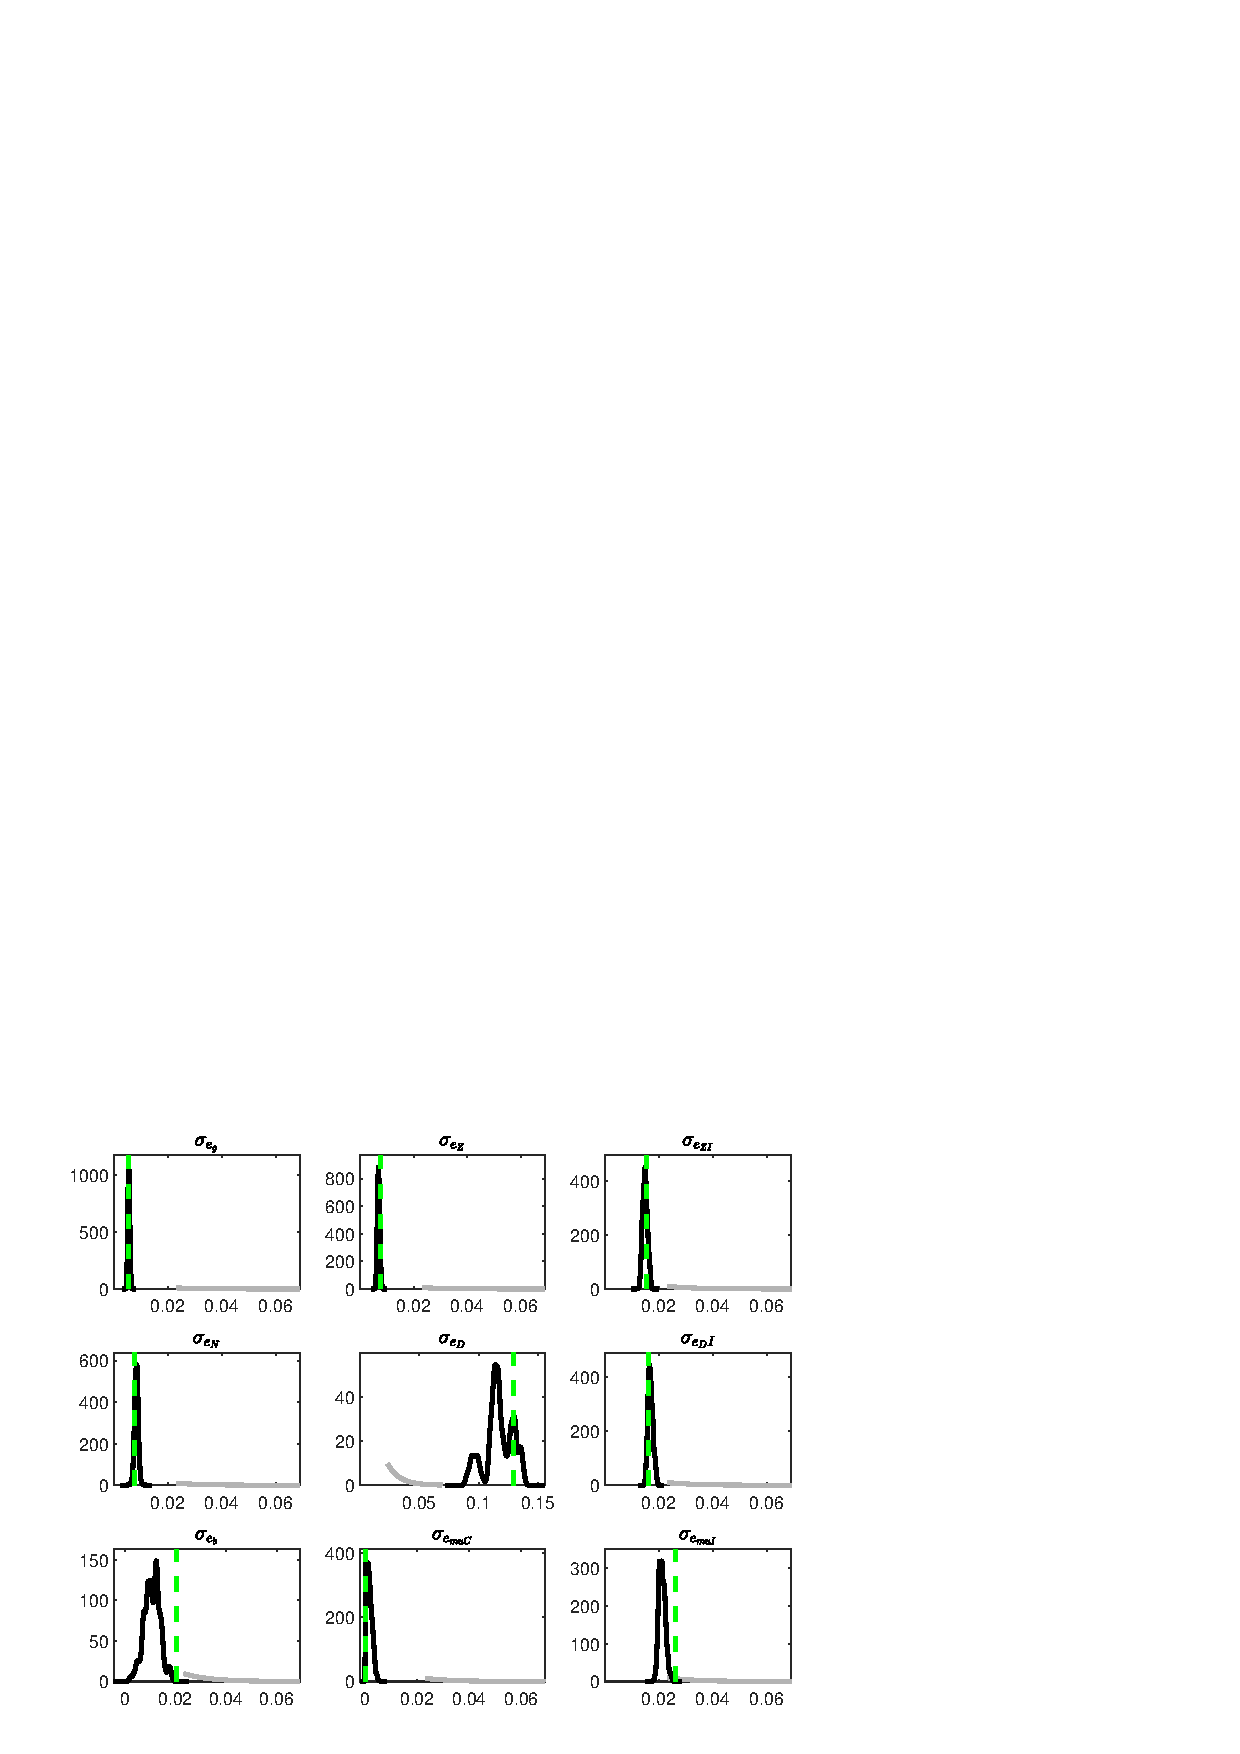
\includegraphics[width=0.80\textwidth]{BRS_sectoral_artificial_data/Output/BRS_sectoral_artificial_data_PriorsAndPosteriors1}
\caption{Priors and posteriors.}\label{Fig:PriorsAndPosteriors:1}
\end{figure}
 
\begin{figure}[H]
\centering
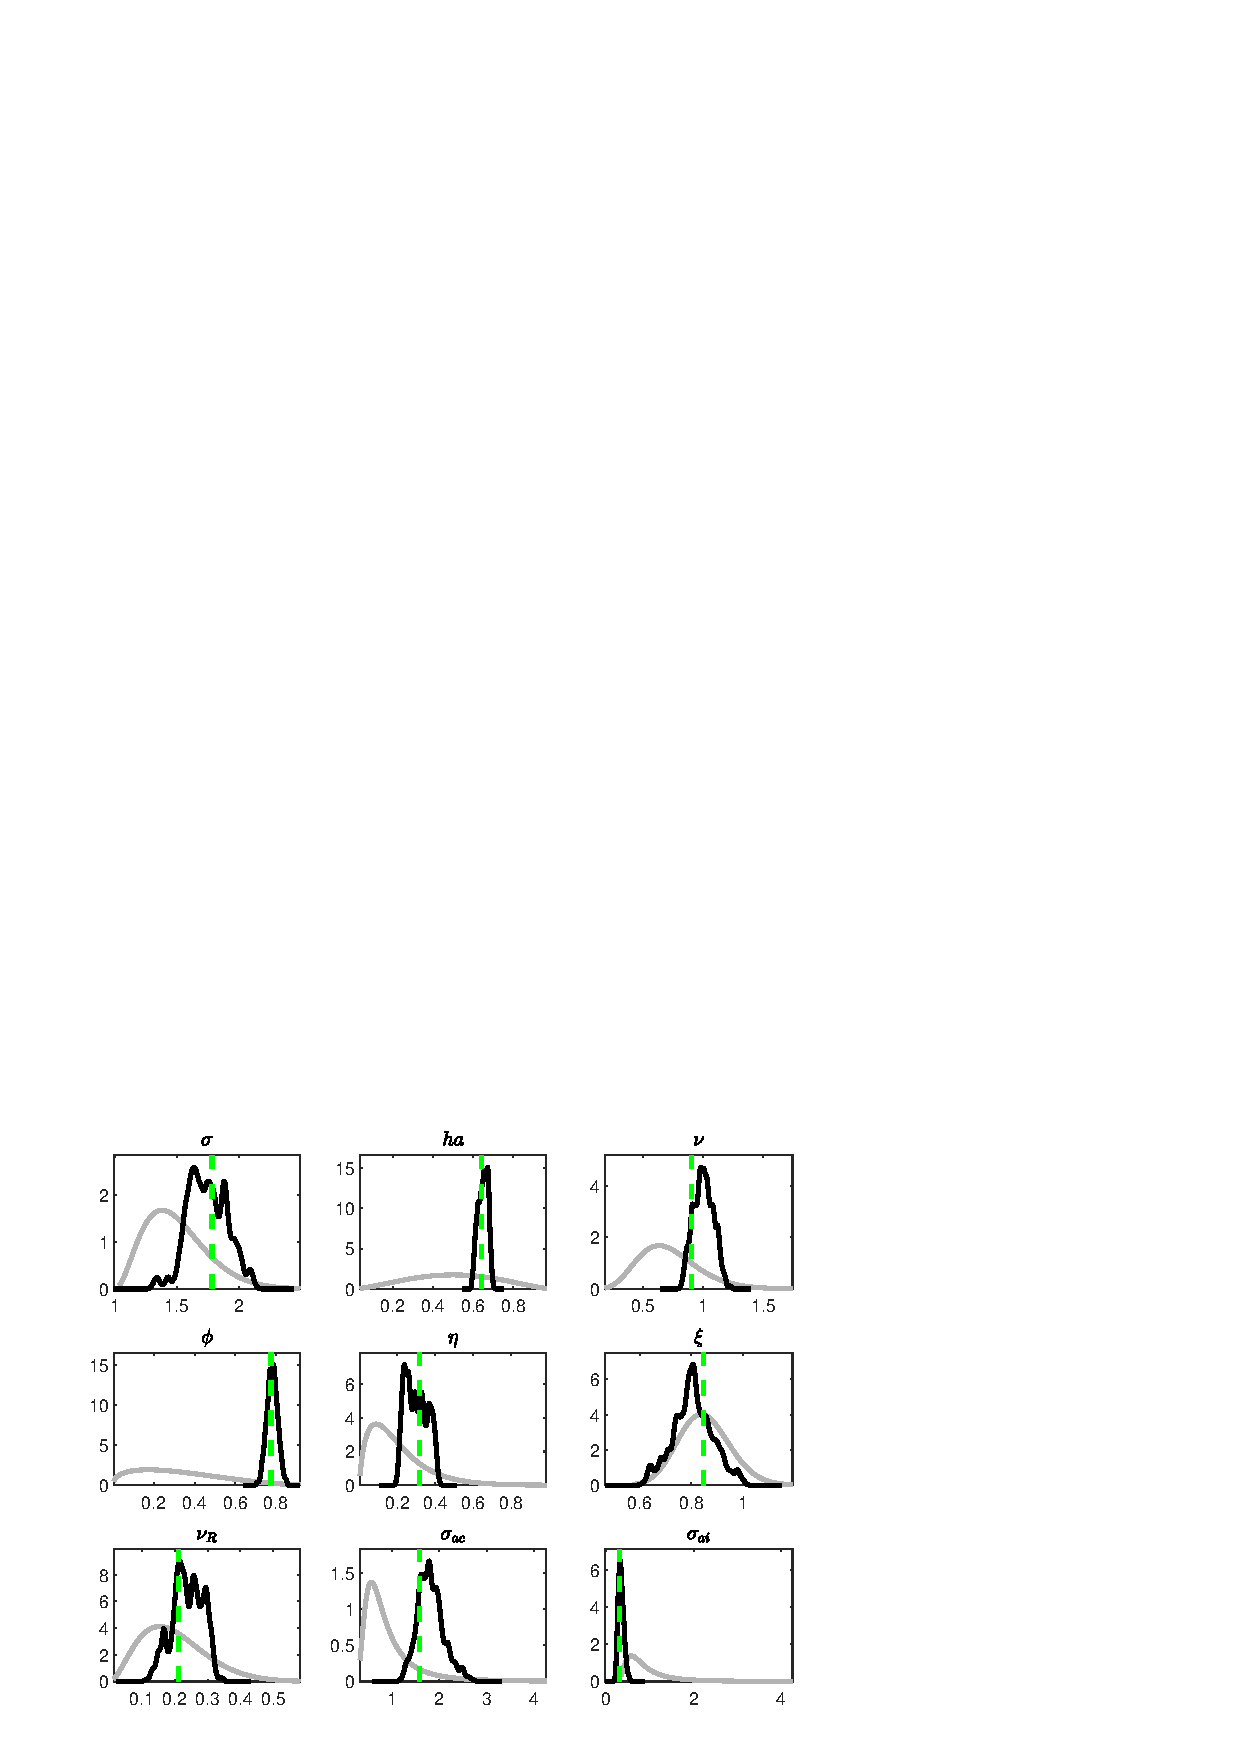
\includegraphics[width=0.80\textwidth]{BRS_sectoral_artificial_data/Output/BRS_sectoral_artificial_data_PriorsAndPosteriors2}
\caption{Priors and posteriors.}\label{Fig:PriorsAndPosteriors:2}
\end{figure}
 
\begin{figure}[H]
\centering
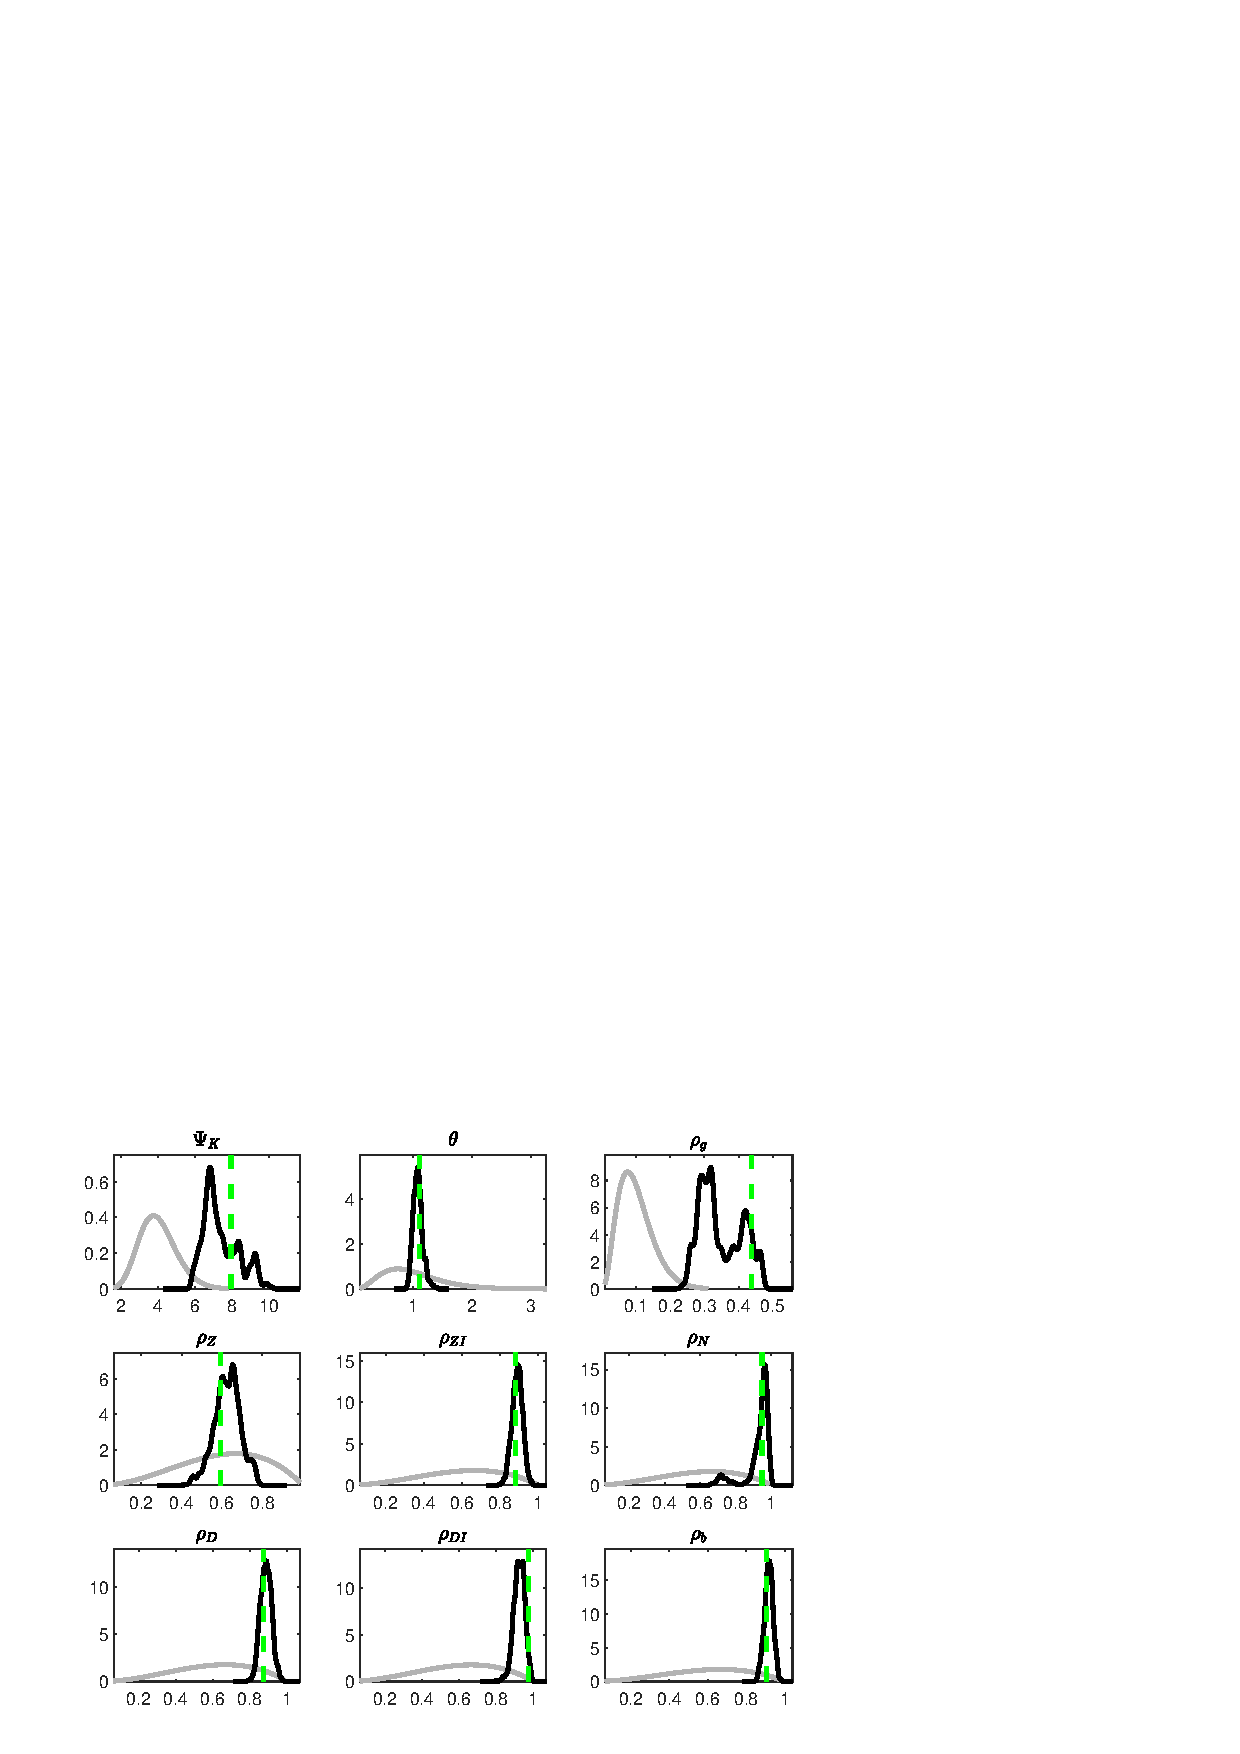
\includegraphics[width=0.80\textwidth]{BRS_sectoral_artificial_data/Output/BRS_sectoral_artificial_data_PriorsAndPosteriors3}
\caption{Priors and posteriors.}\label{Fig:PriorsAndPosteriors:3}
\end{figure}
 
\begin{figure}[H]
\centering
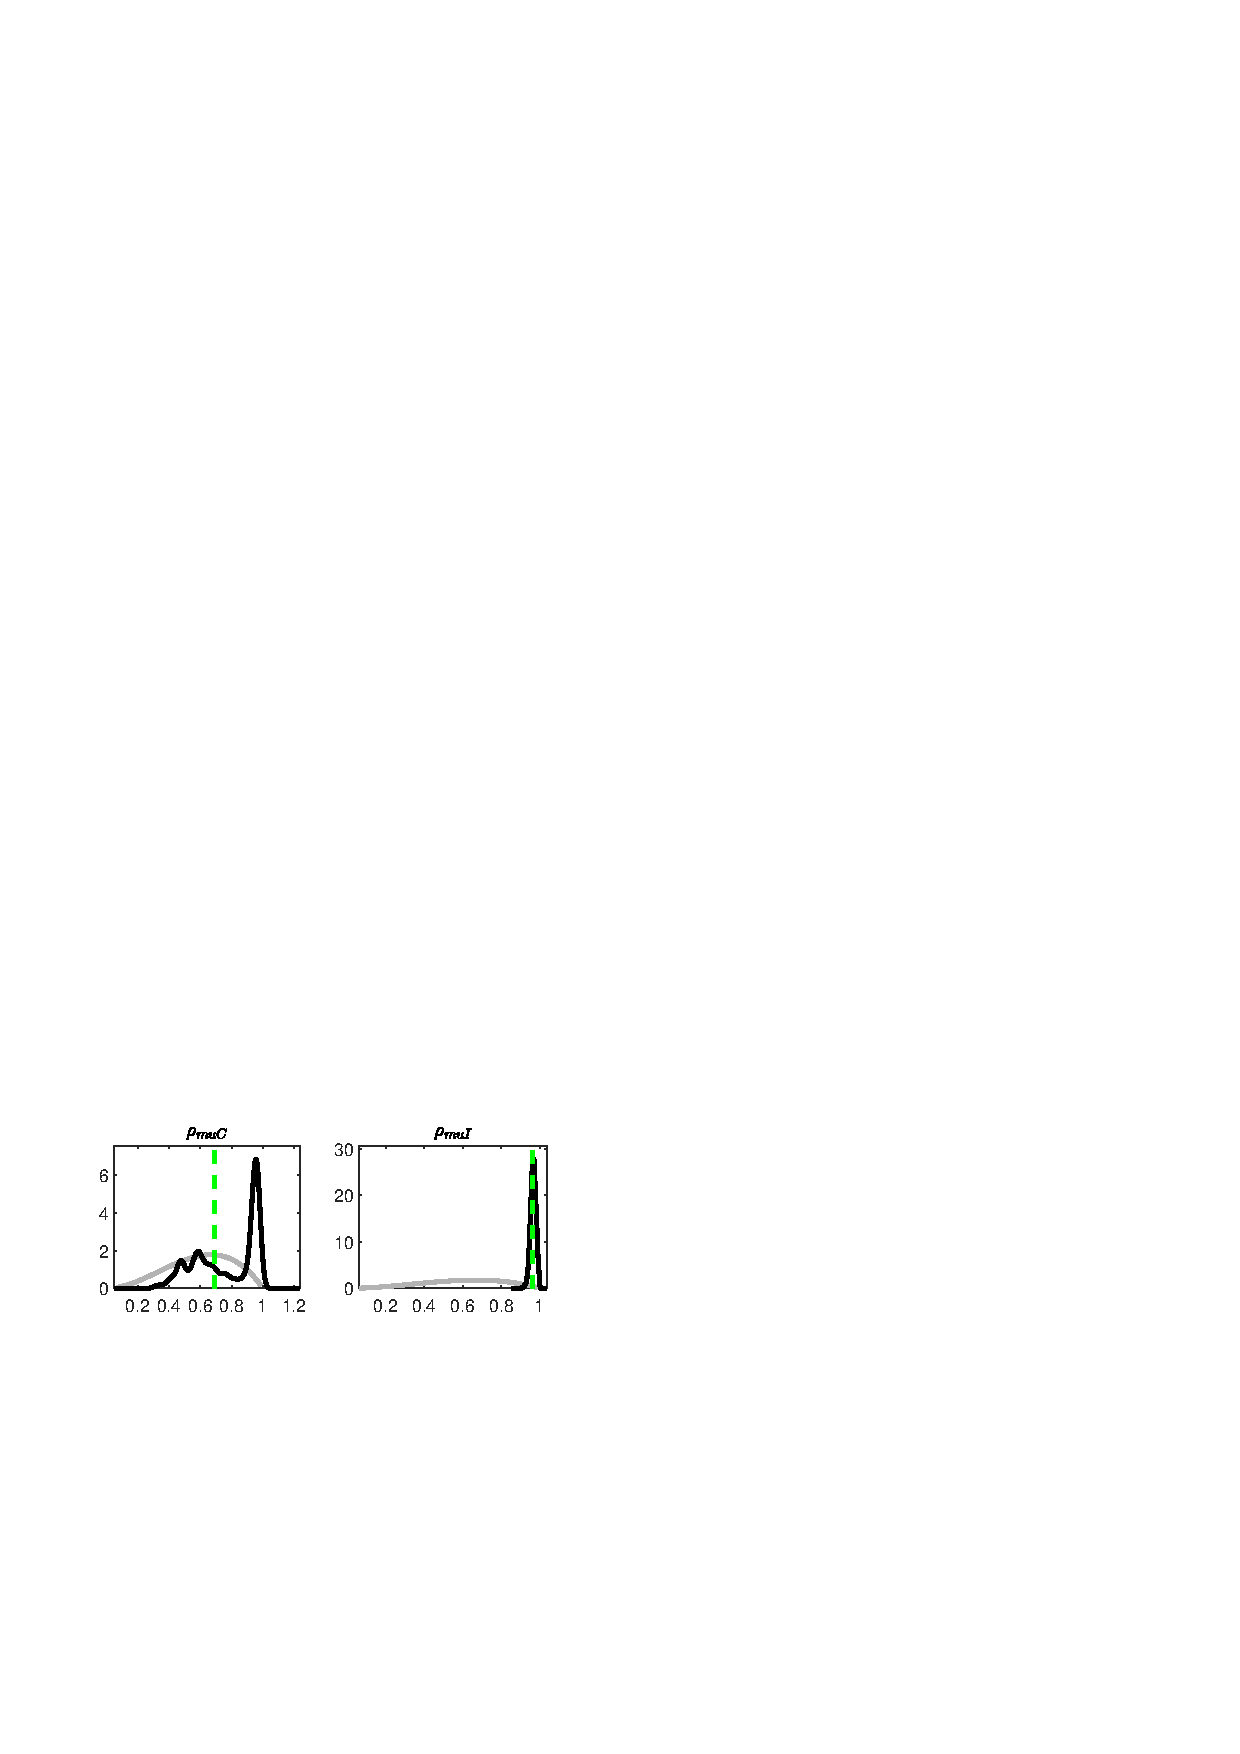
\includegraphics[width=0.53\textwidth]{BRS_sectoral_artificial_data/Output/BRS_sectoral_artificial_data_PriorsAndPosteriors4}
\caption{Priors and posteriors.}\label{Fig:PriorsAndPosteriors:4}
\end{figure}
 
% End of TeX file.
 
% TeX eps-loader file generated by mcmc_diagnostics.m (Dynare).
% 27-Jul-2025 17:52:36
 
\begin{figure}[H]
\centering 
\includegraphics[width=0.80\textwidth]{SU_sectoral_artificial_data/graphs/SU_sectoral_artificial_data_udiag1}
\caption{Univariate convergence diagnostics for the Metropolis-Hastings.
The first, second and third columns are respectively the criteria based on
the eighty percent interval, the second and third moments.}\label{Fig:UnivariateDiagnostics:1}
\end{figure}

\begin{figure}[H]
\centering 
\includegraphics[width=0.80\textwidth]{SU_sectoral_artificial_data/graphs/SU_sectoral_artificial_data_udiag2}
\caption{Univariate convergence diagnostics for the Metropolis-Hastings.
The first, second and third columns are respectively the criteria based on
the eighty percent interval, the second and third moments.}\label{Fig:UnivariateDiagnostics:2}
\end{figure}

\begin{figure}[H]
\centering 
\includegraphics[width=0.80\textwidth]{SU_sectoral_artificial_data/graphs/SU_sectoral_artificial_data_udiag3}
\caption{Univariate convergence diagnostics for the Metropolis-Hastings.
The first, second and third columns are respectively the criteria based on
the eighty percent interval, the second and third moments.}\label{Fig:UnivariateDiagnostics:3}
\end{figure}

\begin{figure}[H]
\centering 
\includegraphics[width=0.80\textwidth]{SU_sectoral_artificial_data/graphs/SU_sectoral_artificial_data_udiag4}
\caption{Univariate convergence diagnostics for the Metropolis-Hastings.
The first, second and third columns are respectively the criteria based on
the eighty percent interval, the second and third moments.}\label{Fig:UnivariateDiagnostics:4}
\end{figure}

\begin{figure}[H]
\centering 
\includegraphics[width=0.80\textwidth]{SU_sectoral_artificial_data/graphs/SU_sectoral_artificial_data_udiag5}
\caption{Univariate convergence diagnostics for the Metropolis-Hastings.
The first, second and third columns are respectively the criteria based on
the eighty percent interval, the second and third moments.}\label{Fig:UnivariateDiagnostics:5}
\end{figure}

\begin{figure}[H]
\centering 
\includegraphics[width=0.80\textwidth]{SU_sectoral_artificial_data/graphs/SU_sectoral_artificial_data_udiag6}
\caption{Univariate convergence diagnostics for the Metropolis-Hastings.
The first, second and third columns are respectively the criteria based on
the eighty percent interval, the second and third moments.}\label{Fig:UnivariateDiagnostics:6}
\end{figure}

\begin{figure}[H]
\centering 
\includegraphics[width=0.80\textwidth]{SU_sectoral_artificial_data/graphs/SU_sectoral_artificial_data_udiag7}
\caption{Univariate convergence diagnostics for the Metropolis-Hastings.
The first, second and third columns are respectively the criteria based on
the eighty percent interval, the second and third moments.}\label{Fig:UnivariateDiagnostics:7}
\end{figure}

\begin{figure}[H]
\centering 
\includegraphics[width=0.80\textwidth]{SU_sectoral_artificial_data/graphs/SU_sectoral_artificial_data_udiag8}
\caption{Univariate convergence diagnostics for the Metropolis-Hastings.
The first, second and third columns are respectively the criteria based on
the eighty percent interval, the second and third moments.}\label{Fig:UnivariateDiagnostics:8}
\end{figure}

\begin{figure}[H]
\centering 
\includegraphics[width=0.80\textwidth]{SU_sectoral_artificial_data/graphs/SU_sectoral_artificial_data_udiag9}
\caption{Univariate convergence diagnostics for the Metropolis-Hastings.
The first, second and third columns are respectively the criteria based on
the eighty percent interval, the second and third moments.}\label{Fig:UnivariateDiagnostics:9}
\end{figure}

\begin{figure}[H]
\centering 
\includegraphics[width=0.80\textwidth]{SU_sectoral_artificial_data/graphs/SU_sectoral_artificial_data_udiag10}
\caption{Univariate convergence diagnostics for the Metropolis-Hastings.
The first, second and third columns are respectively the criteria based on
the eighty percent interval, the second and third moments.}\label{Fig:UnivariateDiagnostics:10}
\end{figure}

% End Of TeX file. 
% TeX eps-loader file generated by mode_check.m (Dynare).
% 27-Jul-2025 17:49:53
 
\begin{figure}[H]
\centering 
\includegraphics[width=0.80\textwidth]{SU_sectoral_artificial_data/graphs/SU_sectoral_artificial_data_CheckPlots1}
\caption{Check plots.}\label{Fig:CheckPlots:1}
\end{figure}
 
\begin{figure}[H]
\centering 
\includegraphics[width=0.80\textwidth]{SU_sectoral_artificial_data/graphs/SU_sectoral_artificial_data_CheckPlots2}
\caption{Check plots.}\label{Fig:CheckPlots:2}
\end{figure}
 
\begin{figure}[H]
\centering 
\includegraphics[width=0.80\textwidth]{SU_sectoral_artificial_data/graphs/SU_sectoral_artificial_data_CheckPlots3}
\caption{Check plots.}\label{Fig:CheckPlots:3}
\end{figure}
 
\begin{figure}[H]
\centering 
\includegraphics[width=0.53\textwidth]{SU_sectoral_artificial_data/graphs/SU_sectoral_artificial_data_CheckPlots4}
\caption{Check plots.}\label{Fig:CheckPlots:4}
\end{figure}
 
 
% TeX eps-loader file generated by dynare_estimation_1.m (Dynare).
% 15-May-2025 16:30:39
 
\begin{figure}[H]
\centering 
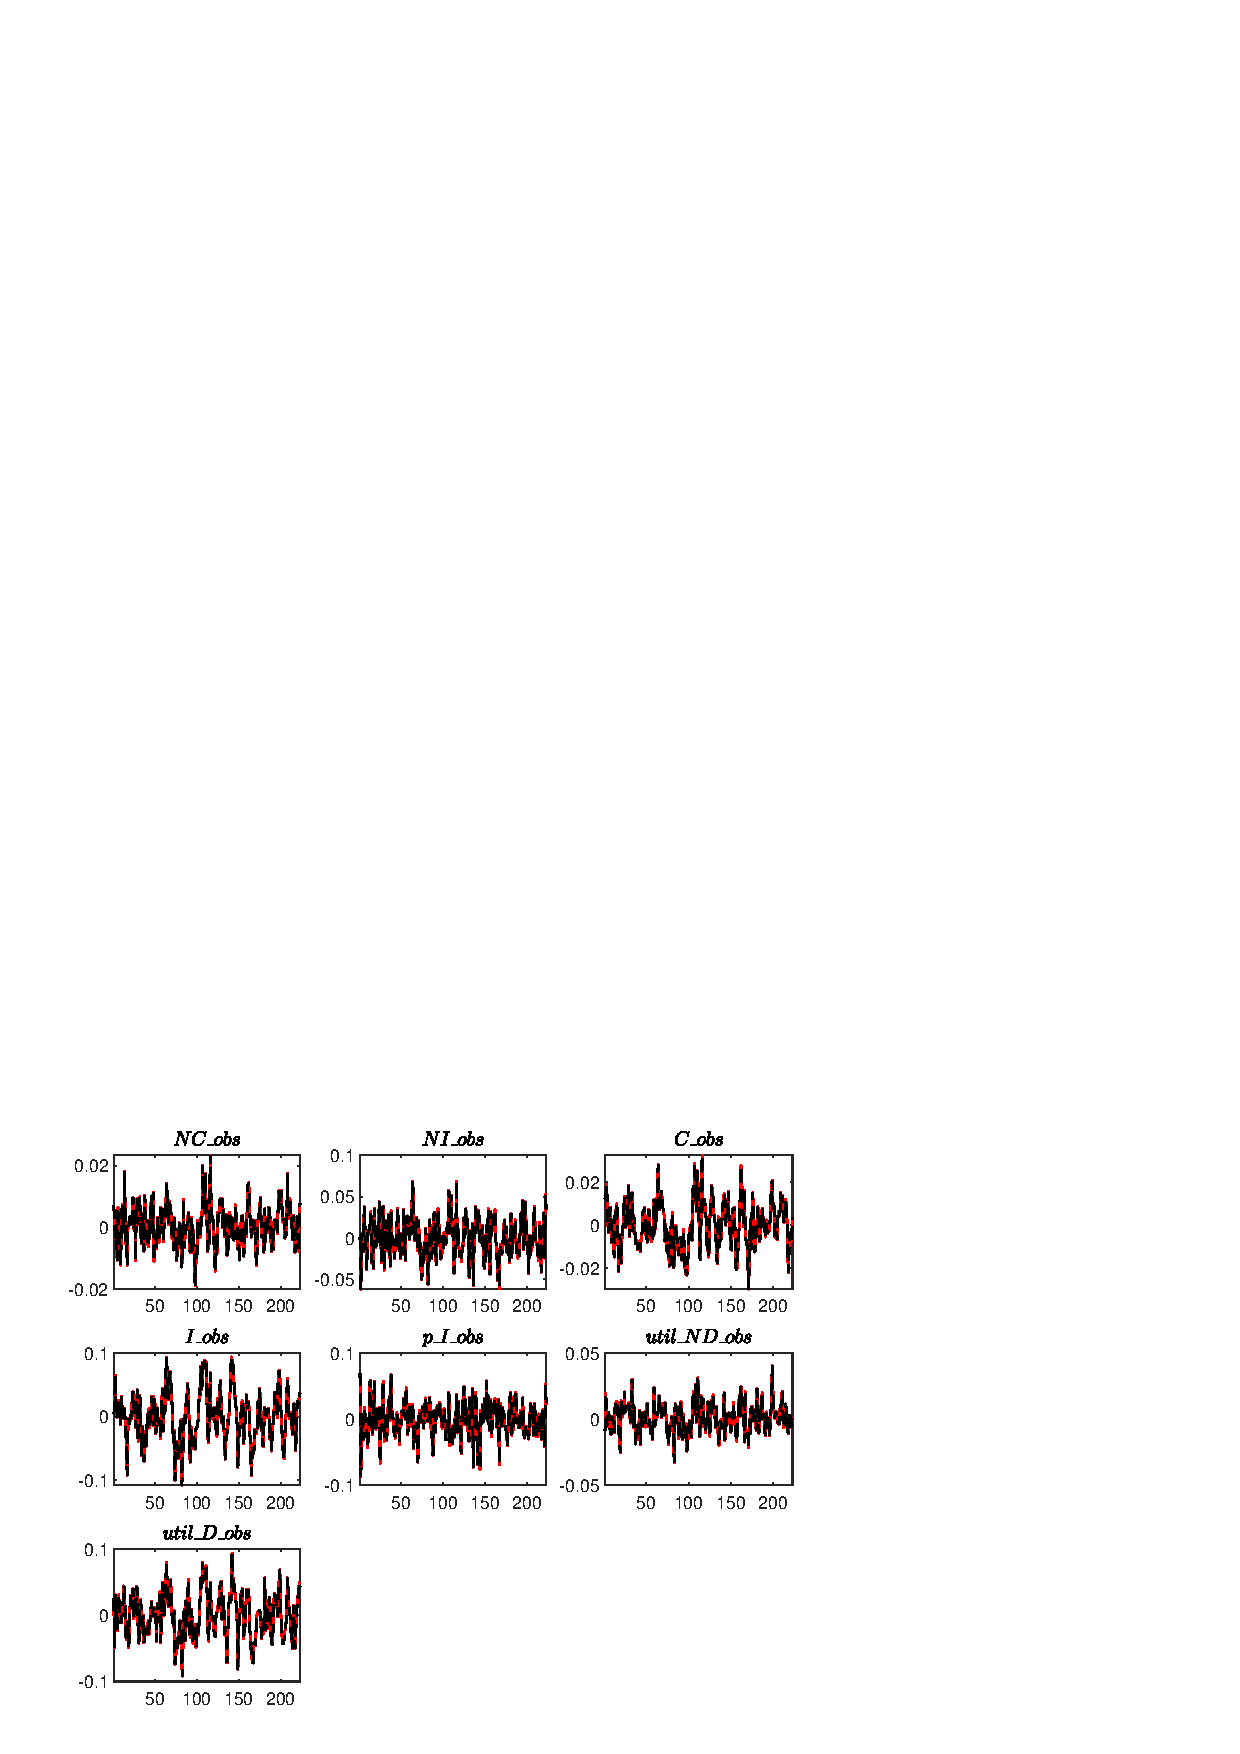
\includegraphics[width=0.80\textwidth]{BRS_sectoral_artificial_data/graphs/BRS_sectoral_artificial_data_HistoricalAndSmoothedVariables1}
\caption{Historical and smoothed variables.}\label{Fig:HistoricalAndSmoothedVariables:1}
\end{figure}


% End of TeX file.
 
% TeX eps-loader file generated by stoch_simul.m (Dynare).
% 02-May-2024 14:11:19
 
\begin{figure}[H]
\centering 
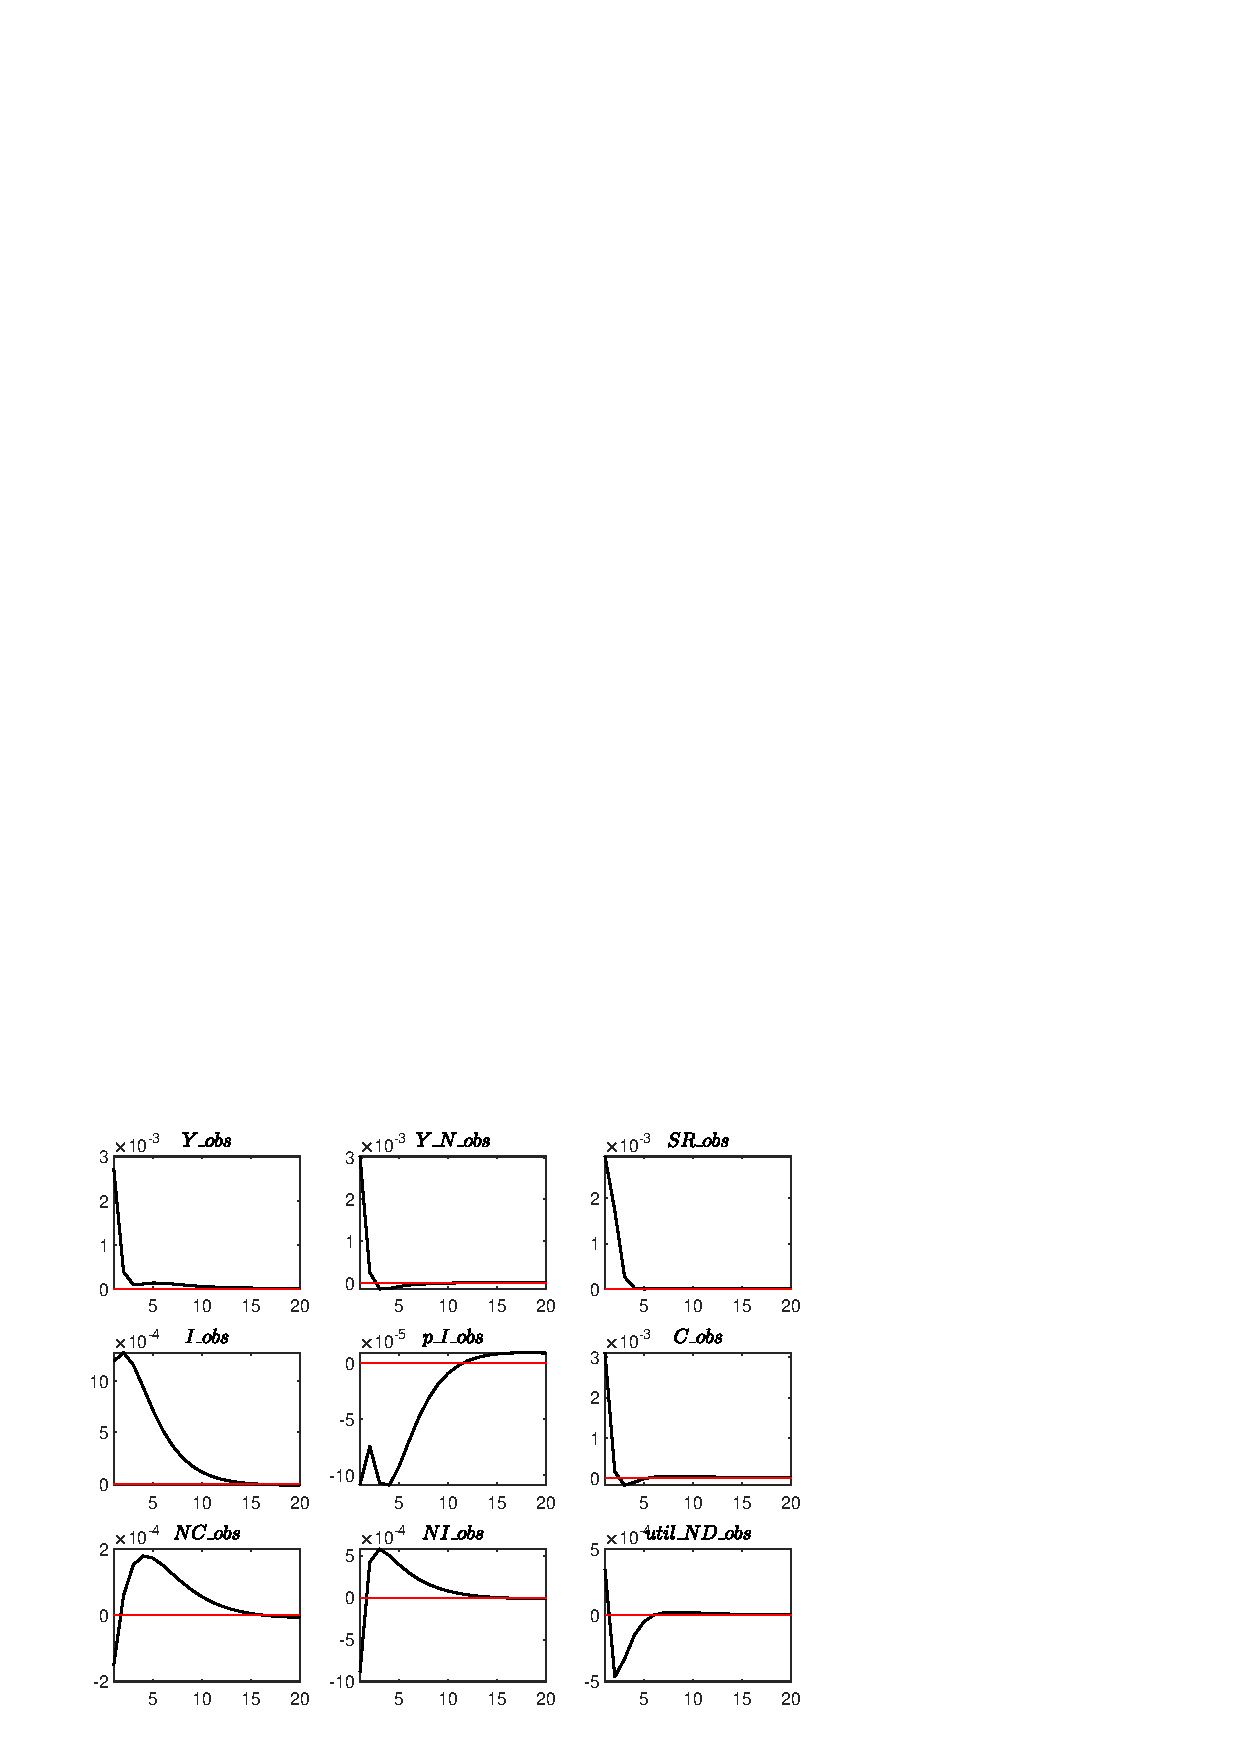
\includegraphics[width=0.80\textwidth]{BRS_sectoral_artificial_data/graphs/BRS_sectoral_artificial_data_IRF_e_g1}
\caption{Impulse response functions (orthogonalized shock to ${e_g}$).}\label{Fig:IRF:e_g:1}
\end{figure}
 
\begin{figure}[H]
\centering 
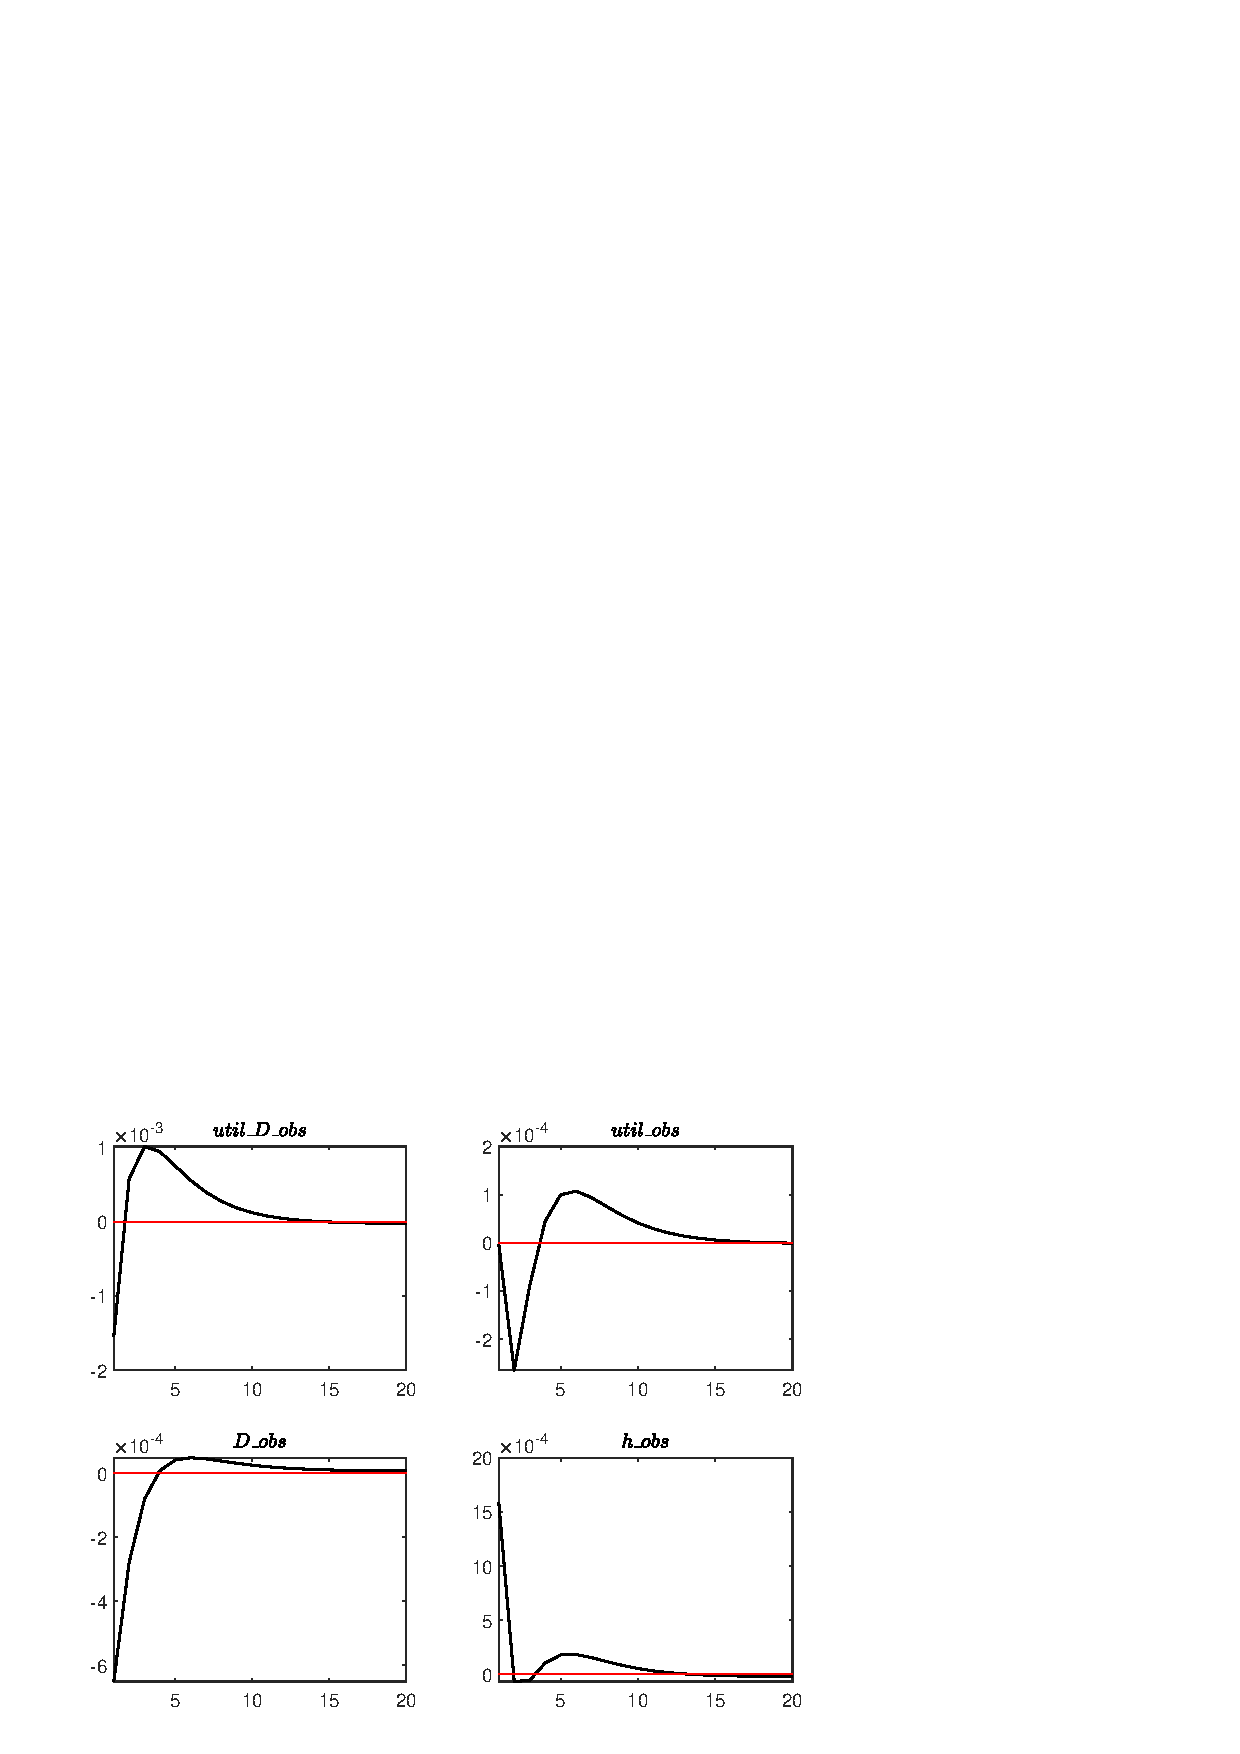
\includegraphics[width=0.80\textwidth]{BRS_sectoral_artificial_data/graphs/BRS_sectoral_artificial_data_IRF_e_g2}
\caption{Impulse response functions (orthogonalized shock to ${e_g}$).}\label{Fig:IRF:e_g:2}
\end{figure}
 
\begin{figure}[H]
\centering 
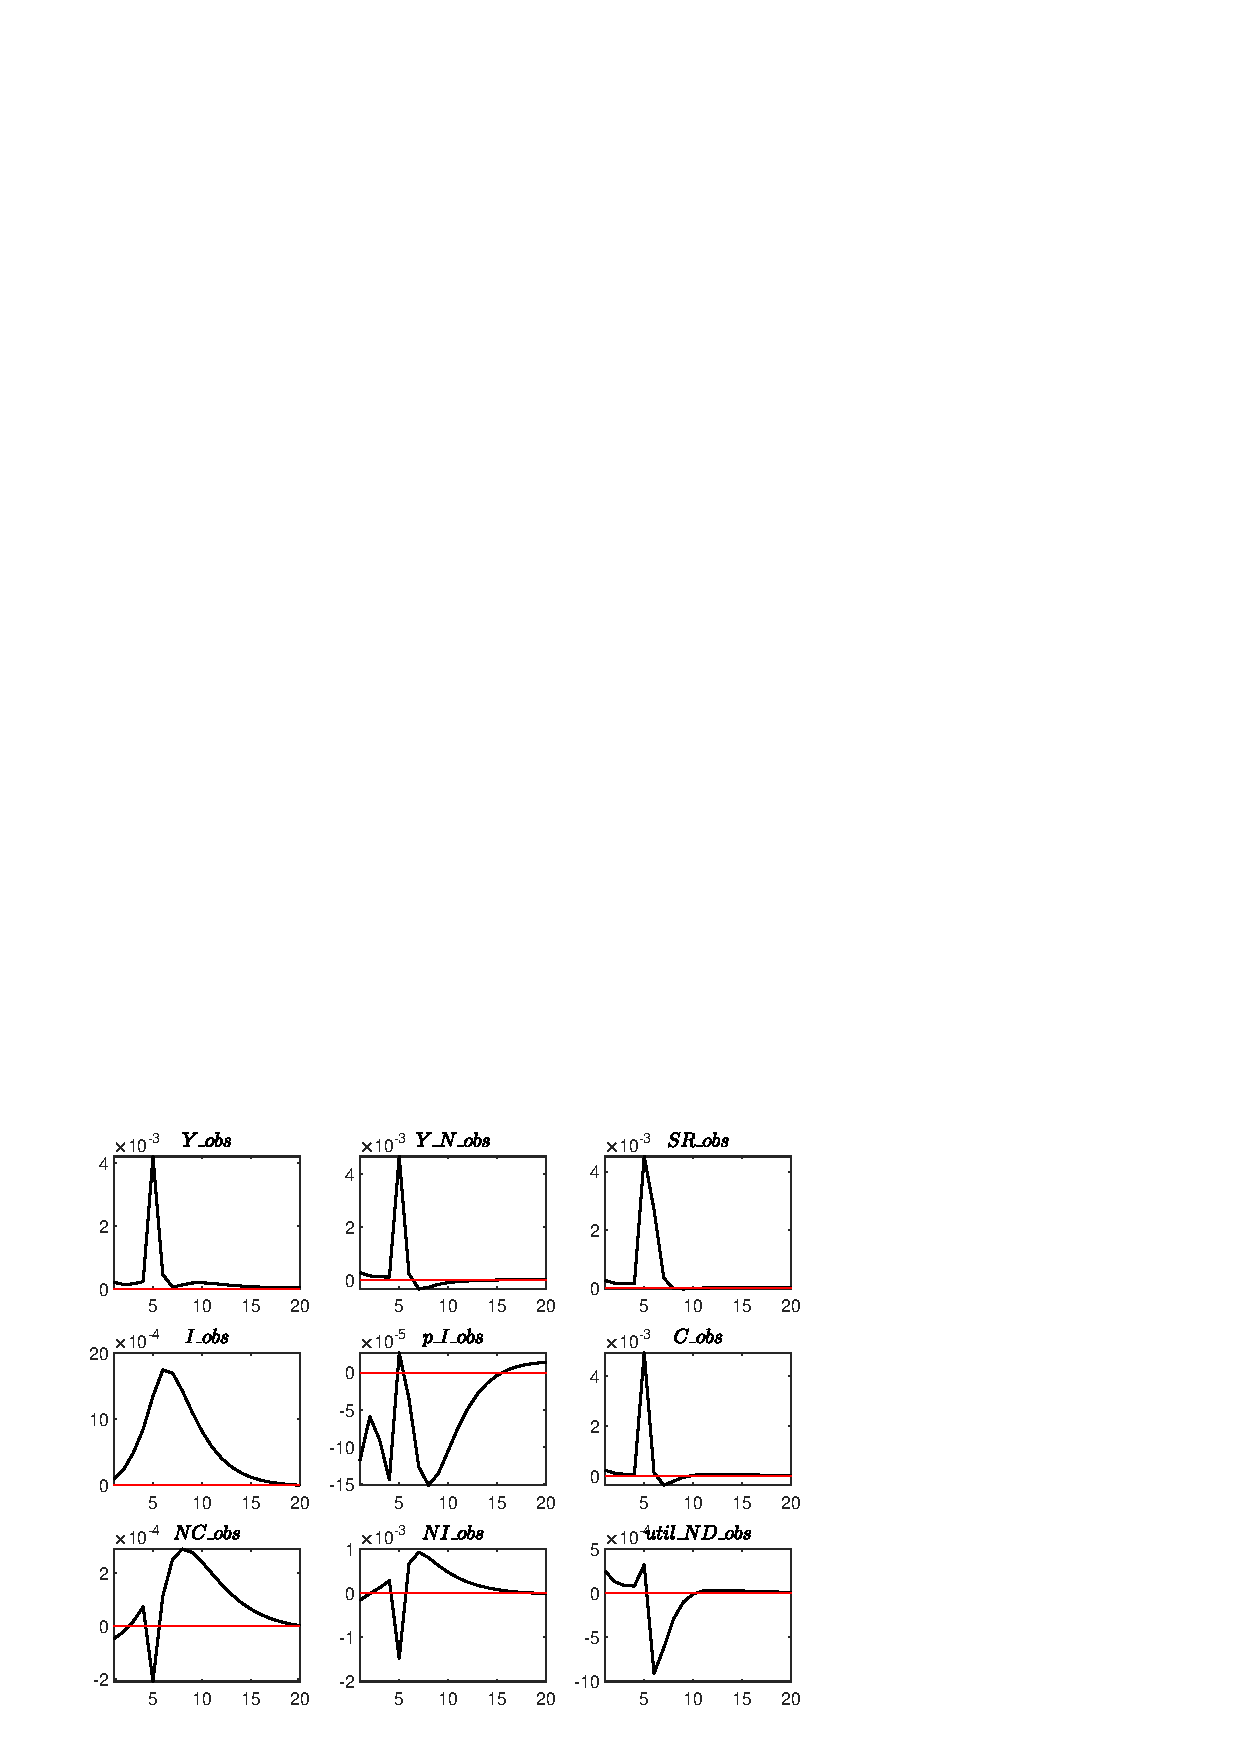
\includegraphics[width=0.80\textwidth]{BRS_sectoral_artificial_data/graphs/BRS_sectoral_artificial_data_IRF_e_g_news1}
\caption{Impulse response functions (orthogonalized shock to ${e_{g,-4}}$).}\label{Fig:IRF:e_g_news:1}
\end{figure}
 
\begin{figure}[H]
\centering 
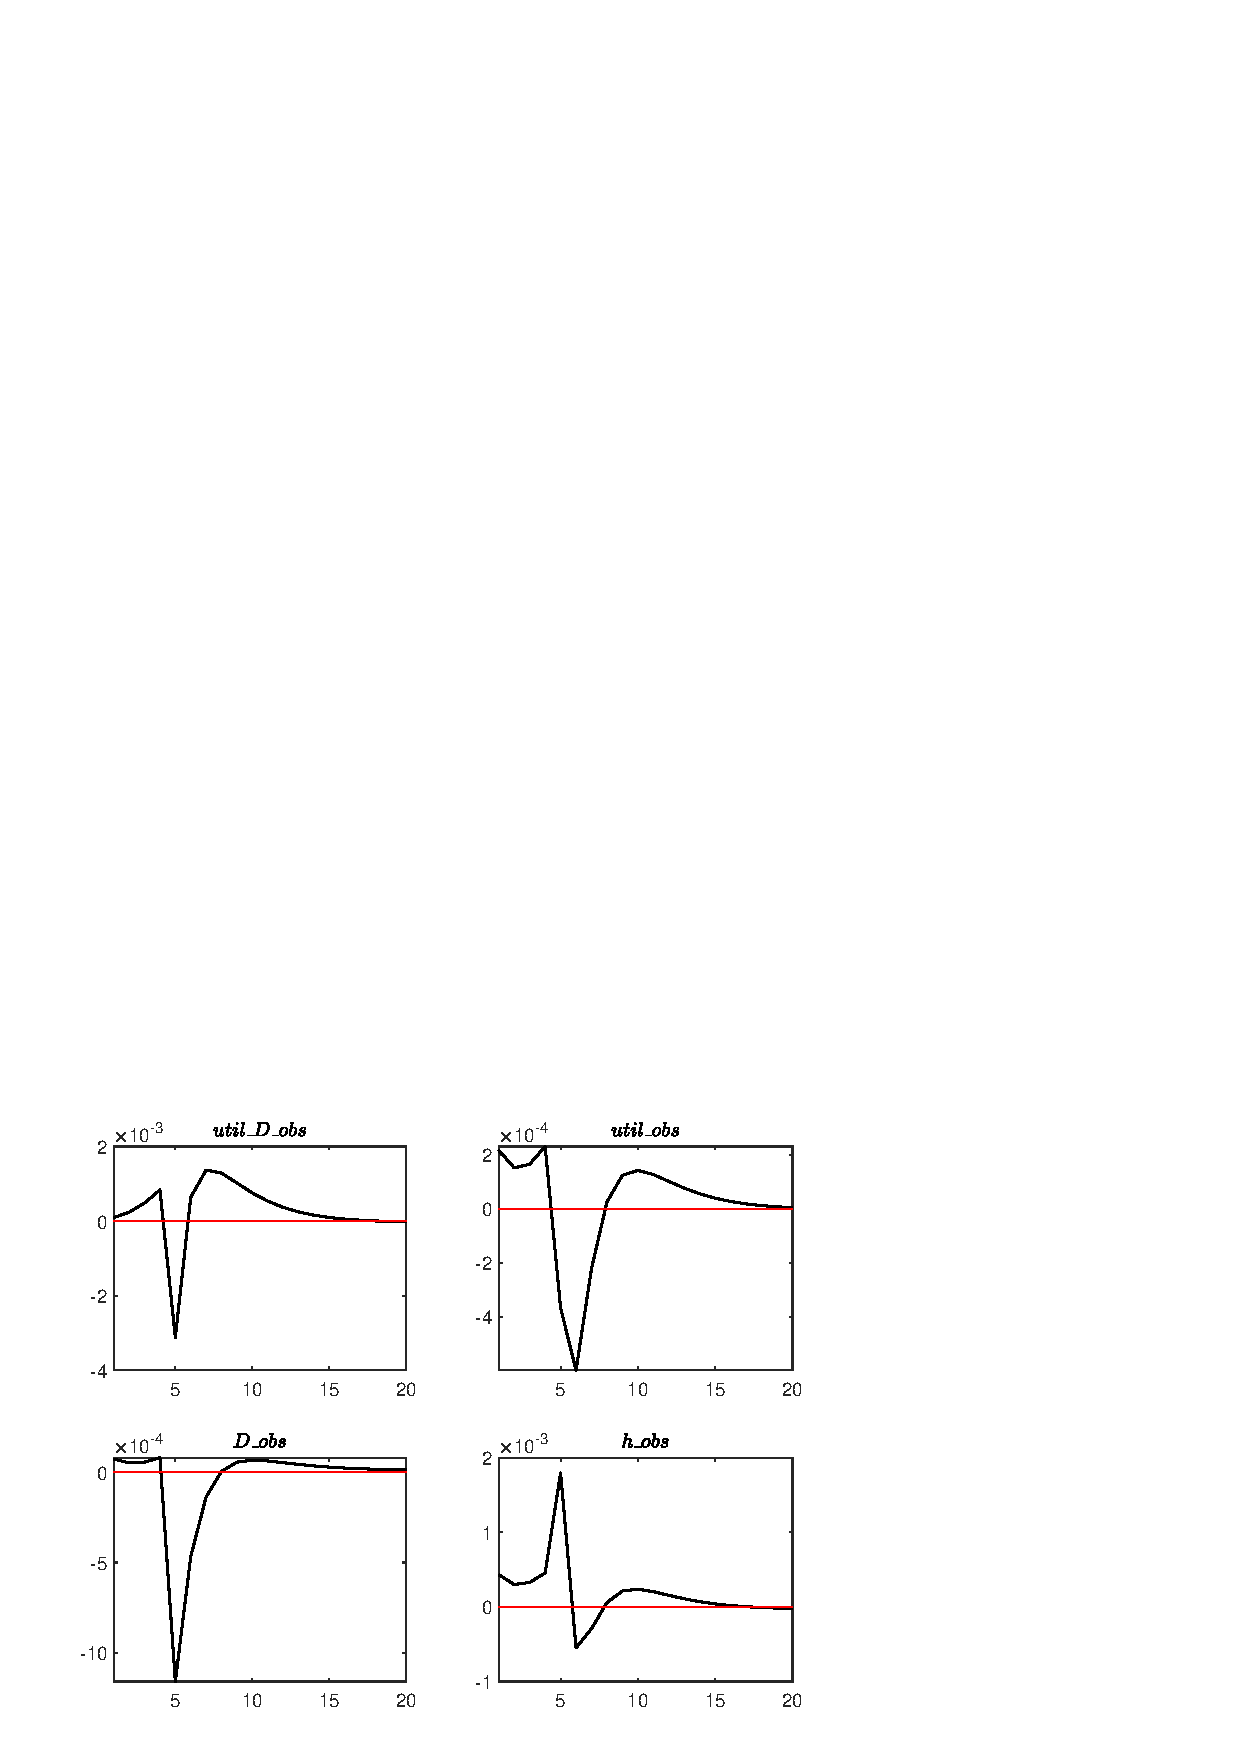
\includegraphics[width=0.80\textwidth]{BRS_sectoral_artificial_data/graphs/BRS_sectoral_artificial_data_IRF_e_g_news2}
\caption{Impulse response functions (orthogonalized shock to ${e_{g,-4}}$).}\label{Fig:IRF:e_g_news:2}
\end{figure}
 
\begin{figure}[H]
\centering 
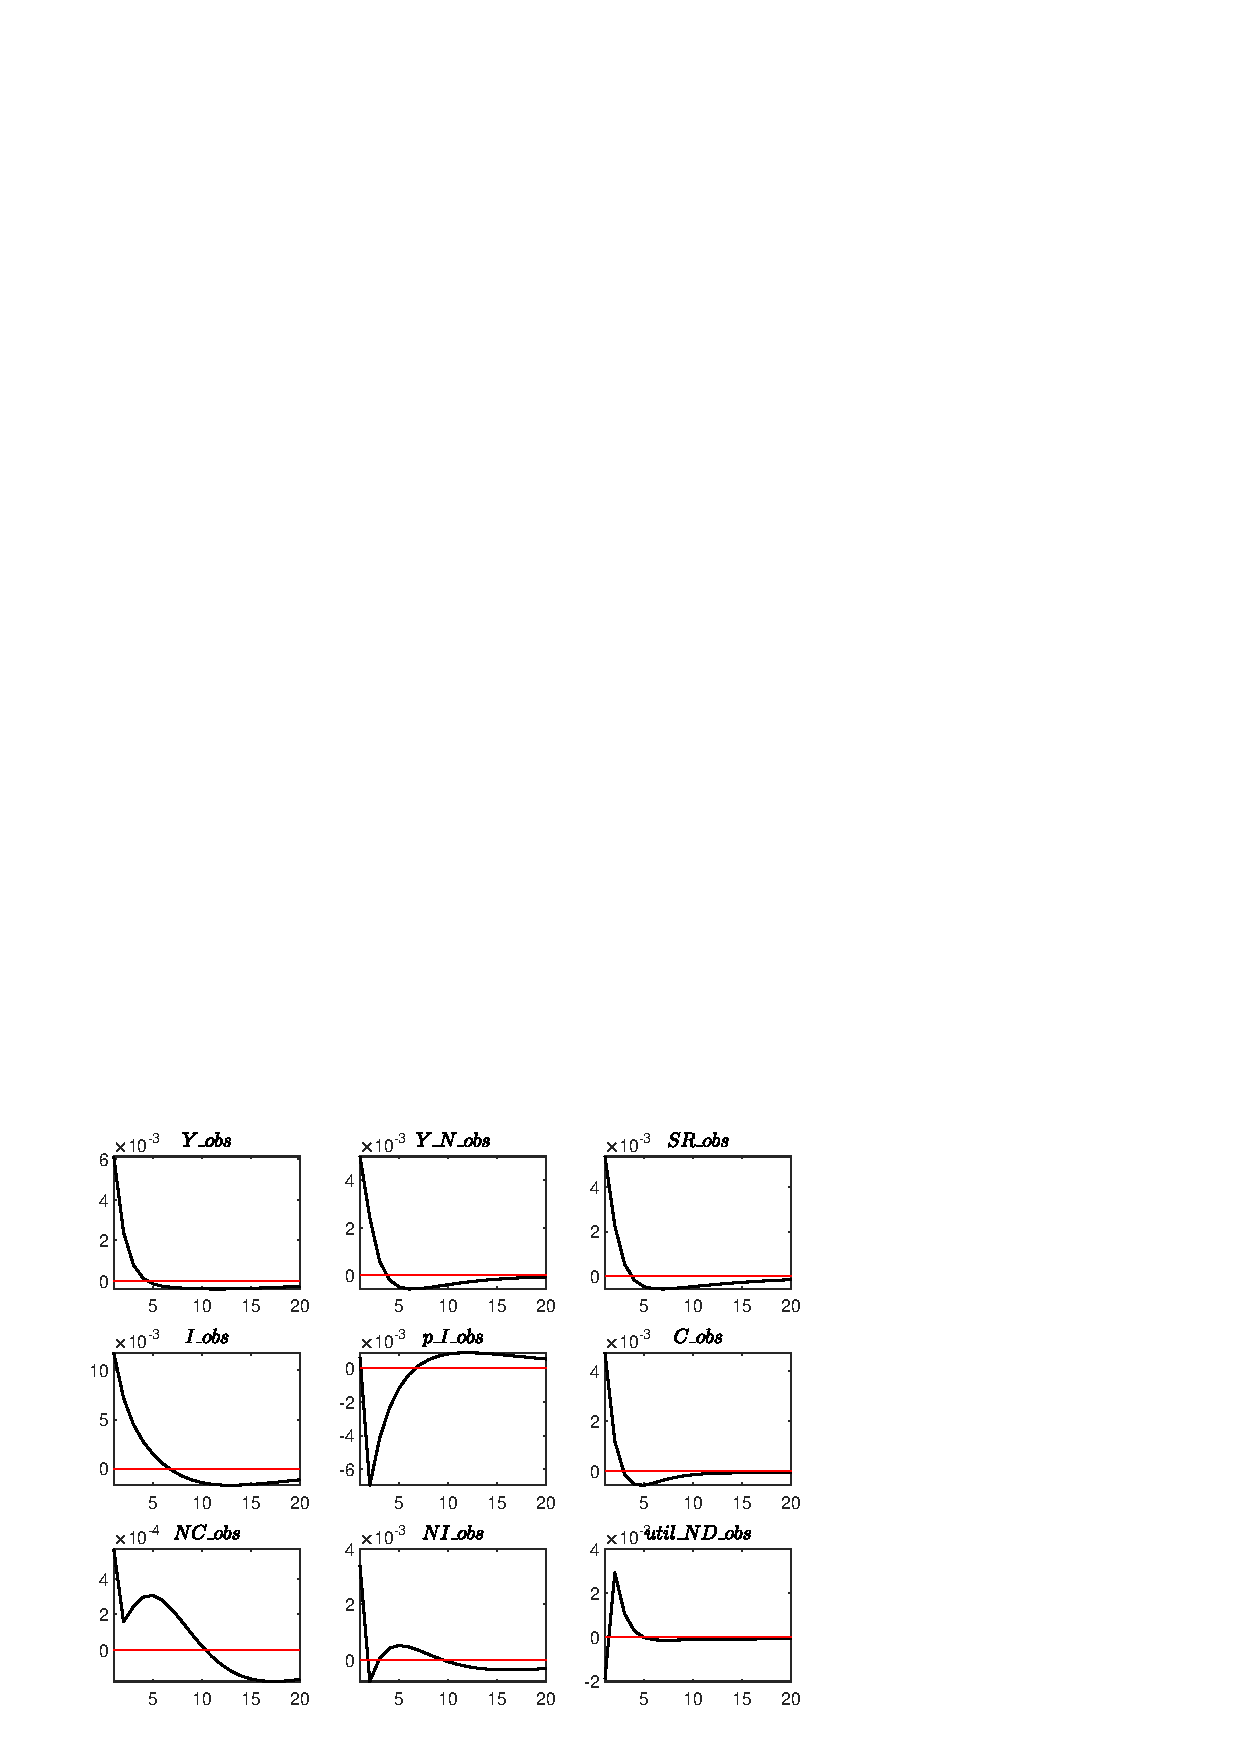
\includegraphics[width=0.80\textwidth]{BRS_sectoral_artificial_data/graphs/BRS_sectoral_artificial_data_IRF_e_Z1}
\caption{Impulse response functions (orthogonalized shock to ${e_Z}$).}\label{Fig:IRF:e_Z:1}
\end{figure}
 
\begin{figure}[H]
\centering 
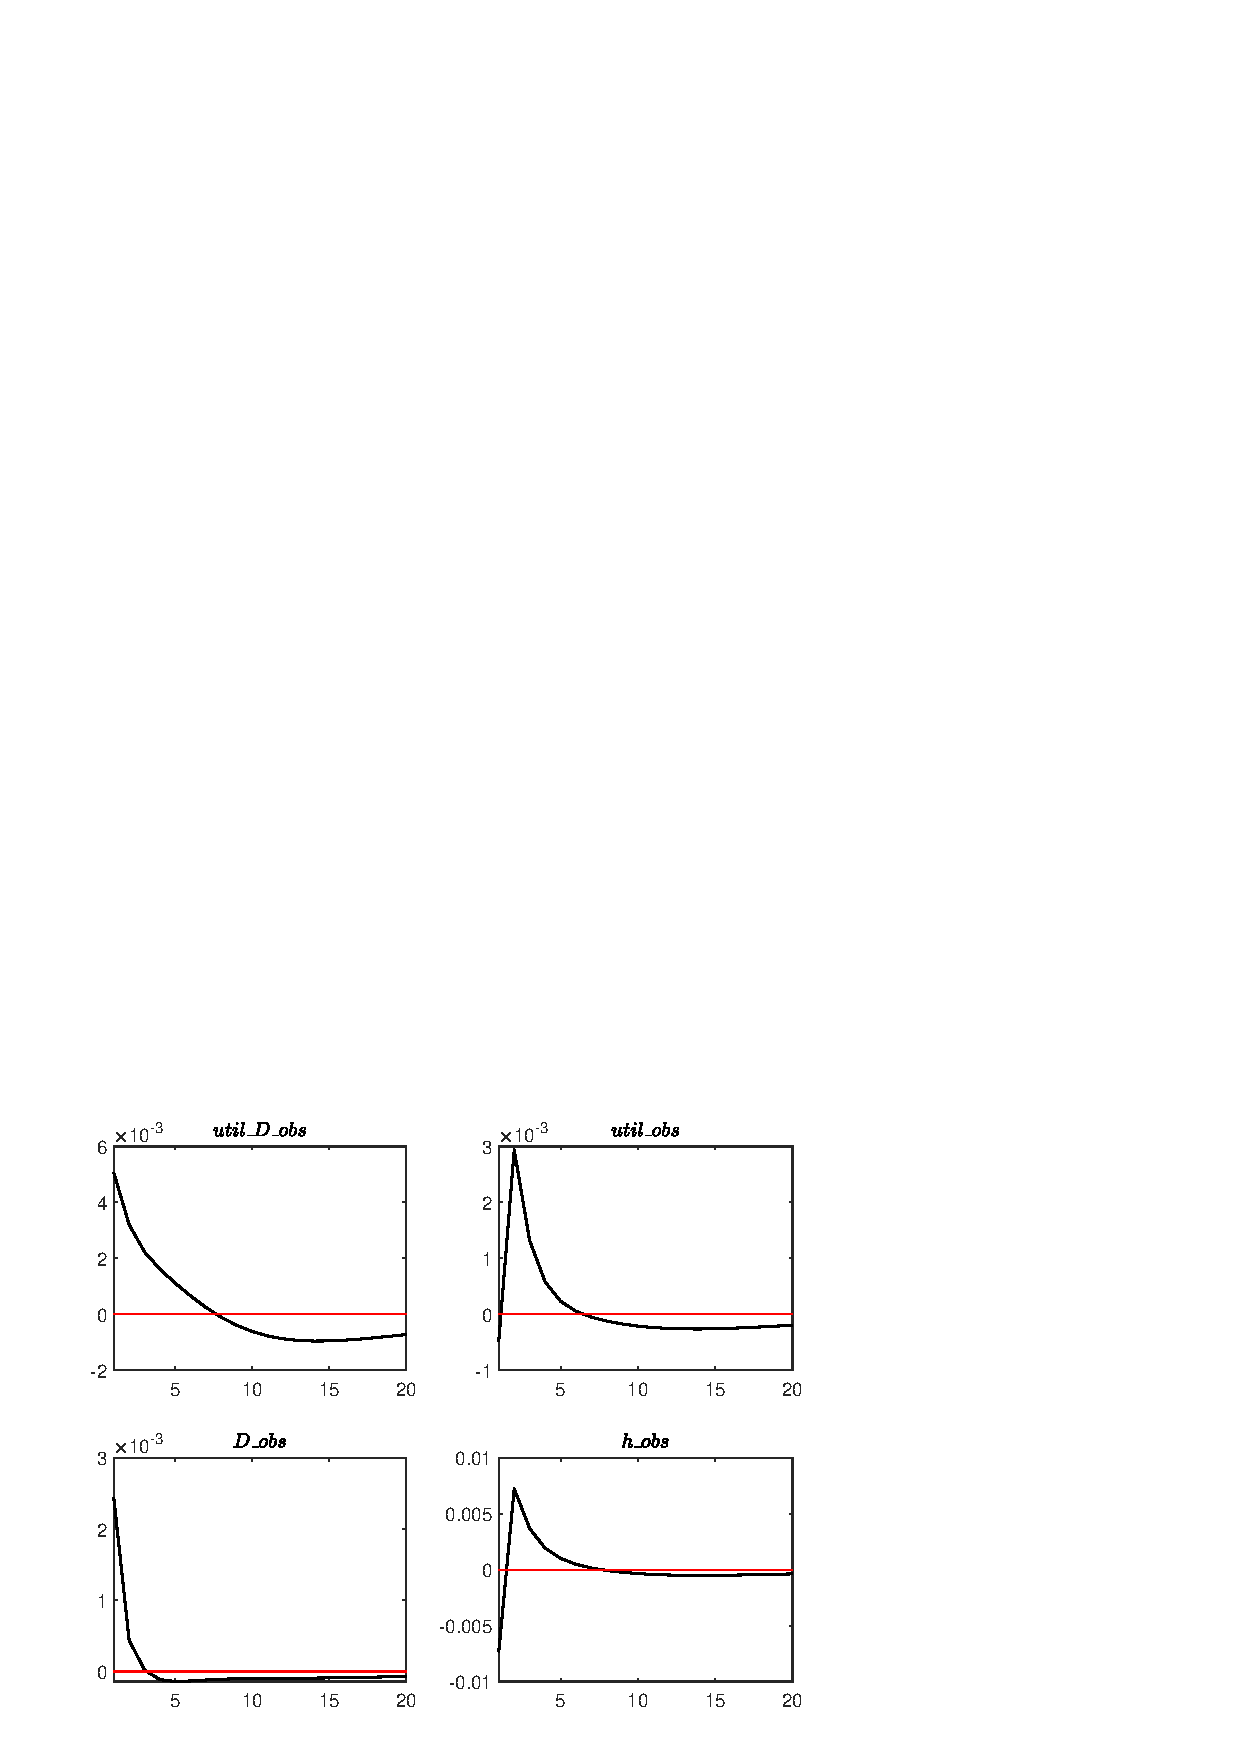
\includegraphics[width=0.80\textwidth]{BRS_sectoral_artificial_data/graphs/BRS_sectoral_artificial_data_IRF_e_Z2}
\caption{Impulse response functions (orthogonalized shock to ${e_Z}$).}\label{Fig:IRF:e_Z:2}
\end{figure}
 
\begin{figure}[H]
\centering 
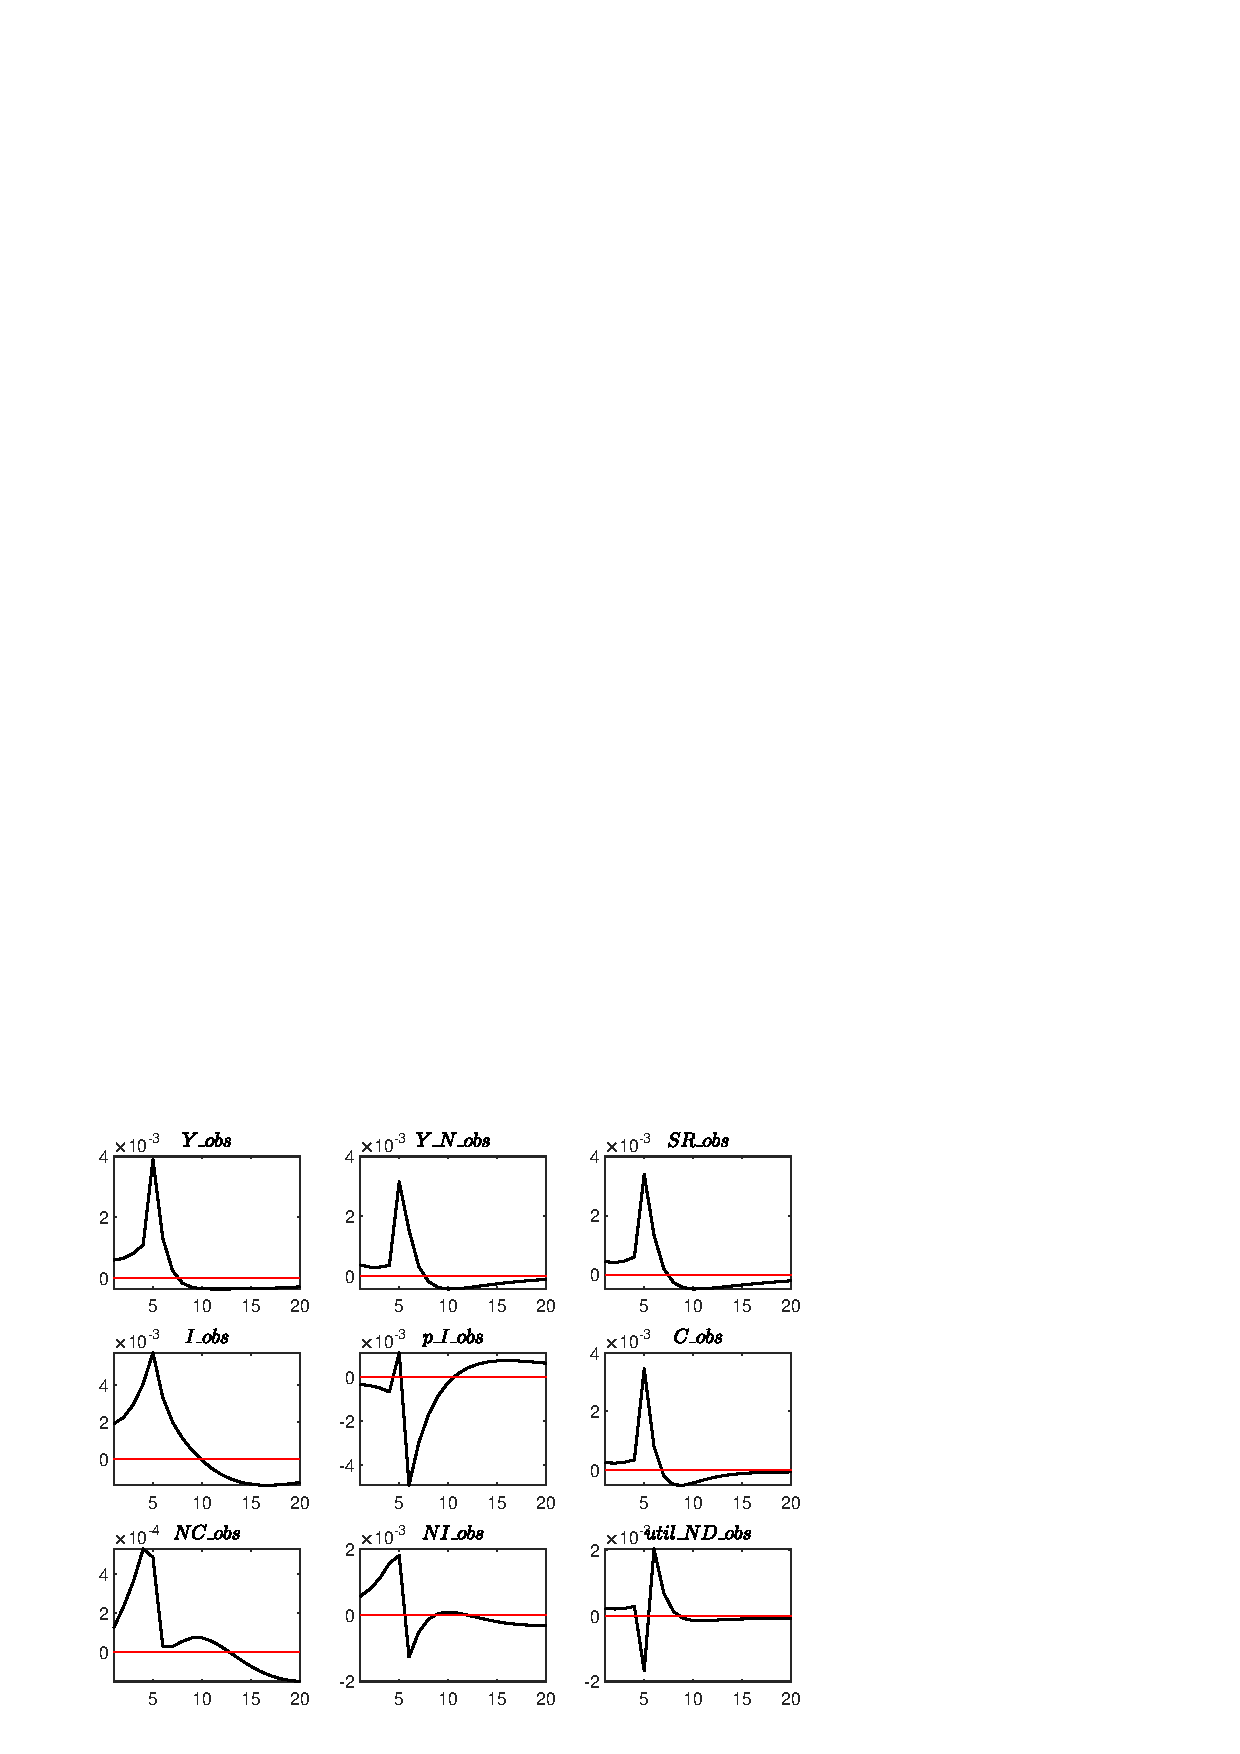
\includegraphics[width=0.80\textwidth]{BRS_sectoral_artificial_data/graphs/BRS_sectoral_artificial_data_IRF_e_Z_news1}
\caption{Impulse response functions (orthogonalized shock to ${e_{Z,-4}}$).}\label{Fig:IRF:e_Z_news:1}
\end{figure}
 
\begin{figure}[H]
\centering 
\includegraphics[width=0.80\textwidth]{BRS_sectoral_artificial_data/graphs/BRS_sectoral_artificial_data_IRF_e_Z_news2}
\caption{Impulse response functions (orthogonalized shock to ${e_{Z,-4}}$).}\label{Fig:IRF:e_Z_news:2}
\end{figure}
 
\begin{figure}[H]
\centering 
\includegraphics[width=0.80\textwidth]{BRS_sectoral_artificial_data/graphs/BRS_sectoral_artificial_data_IRF_e_ZI1}
\caption{Impulse response functions (orthogonalized shock to ${e_{ZI}}$).}\label{Fig:IRF:e_ZI:1}
\end{figure}
 
\begin{figure}[H]
\centering 
\includegraphics[width=0.80\textwidth]{BRS_sectoral_artificial_data/graphs/BRS_sectoral_artificial_data_IRF_e_ZI2}
\caption{Impulse response functions (orthogonalized shock to ${e_{ZI}}$).}\label{Fig:IRF:e_ZI:2}
\end{figure}
 
\begin{figure}[H]
\centering 
\includegraphics[width=0.80\textwidth]{BRS_sectoral_artificial_data/graphs/BRS_sectoral_artificial_data_IRF_e_ZI_news1}
\caption{Impulse response functions (orthogonalized shock to ${e_{ZI,-4}}$).}\label{Fig:IRF:e_ZI_news:1}
\end{figure}
 
\begin{figure}[H]
\centering 
\includegraphics[width=0.80\textwidth]{BRS_sectoral_artificial_data/graphs/BRS_sectoral_artificial_data_IRF_e_ZI_news2}
\caption{Impulse response functions (orthogonalized shock to ${e_{ZI,-4}}$).}\label{Fig:IRF:e_ZI_news:2}
\end{figure}
 
\begin{figure}[H]
\centering 
\includegraphics[width=0.80\textwidth]{BRS_sectoral_artificial_data/graphs/BRS_sectoral_artificial_data_IRF_e_N1}
\caption{Impulse response functions (orthogonalized shock to ${e_N}$).}\label{Fig:IRF:e_N:1}
\end{figure}
 
\begin{figure}[H]
\centering 
\includegraphics[width=0.80\textwidth]{BRS_sectoral_artificial_data/graphs/BRS_sectoral_artificial_data_IRF_e_N2}
\caption{Impulse response functions (orthogonalized shock to ${e_N}$).}\label{Fig:IRF:e_N:2}
\end{figure}
 
\begin{figure}[H]
\centering 
\includegraphics[width=0.80\textwidth]{BRS_sectoral_artificial_data/graphs/BRS_sectoral_artificial_data_IRF_e_D1}
\caption{Impulse response functions (orthogonalized shock to ${e_D}$).}\label{Fig:IRF:e_D:1}
\end{figure}
 
\begin{figure}[H]
\centering 
\includegraphics[width=0.80\textwidth]{BRS_sectoral_artificial_data/graphs/BRS_sectoral_artificial_data_IRF_e_D2}
\caption{Impulse response functions (orthogonalized shock to ${e_D}$).}\label{Fig:IRF:e_D:2}
\end{figure}
 
\begin{figure}[H]
\centering 
\includegraphics[width=0.80\textwidth]{BRS_sectoral_artificial_data/graphs/BRS_sectoral_artificial_data_IRF_e_D_news1}
\caption{Impulse response functions (orthogonalized shock to ${e_{D,4}}$).}\label{Fig:IRF:e_D_news:1}
\end{figure}
 
\begin{figure}[H]
\centering 
\includegraphics[width=0.80\textwidth]{BRS_sectoral_artificial_data/graphs/BRS_sectoral_artificial_data_IRF_e_D_news2}
\caption{Impulse response functions (orthogonalized shock to ${e_{D,4}}$).}\label{Fig:IRF:e_D_news:2}
\end{figure}
 
\begin{figure}[H]
\centering 
\includegraphics[width=0.80\textwidth]{BRS_sectoral_artificial_data/graphs/BRS_sectoral_artificial_data_IRF_e_DI1}
\caption{Impulse response functions (orthogonalized shock to ${e_DI}$).}\label{Fig:IRF:e_DI:1}
\end{figure}
 
\begin{figure}[H]
\centering 
\includegraphics[width=0.80\textwidth]{BRS_sectoral_artificial_data/graphs/BRS_sectoral_artificial_data_IRF_e_DI2}
\caption{Impulse response functions (orthogonalized shock to ${e_DI}$).}\label{Fig:IRF:e_DI:2}
\end{figure}
 
\begin{figure}[H]
\centering 
\includegraphics[width=0.80\textwidth]{BRS_sectoral_artificial_data/graphs/BRS_sectoral_artificial_data_IRF_e_DI_news1}
\caption{Impulse response functions (orthogonalized shock to ${e_{DI,-4}}$).}\label{Fig:IRF:e_DI_news:1}
\end{figure}
 
\begin{figure}[H]
\centering 
\includegraphics[width=0.80\textwidth]{BRS_sectoral_artificial_data/graphs/BRS_sectoral_artificial_data_IRF_e_DI_news2}
\caption{Impulse response functions (orthogonalized shock to ${e_{DI,-4}}$).}\label{Fig:IRF:e_DI_news:2}
\end{figure}
 
\begin{figure}[H]
\centering 
\includegraphics[width=0.80\textwidth]{BRS_sectoral_artificial_data/graphs/BRS_sectoral_artificial_data_IRF_e_b1}
\caption{Impulse response functions (orthogonalized shock to ${e_b}$).}\label{Fig:IRF:e_b:1}
\end{figure}
 
\begin{figure}[H]
\centering 
\includegraphics[width=0.80\textwidth]{BRS_sectoral_artificial_data/graphs/BRS_sectoral_artificial_data_IRF_e_b2}
\caption{Impulse response functions (orthogonalized shock to ${e_b}$).}\label{Fig:IRF:e_b:2}
\end{figure}
 
\begin{figure}[H]
\centering 
\includegraphics[width=0.80\textwidth]{BRS_sectoral_artificial_data/graphs/BRS_sectoral_artificial_data_IRF_e_b_news1}
\caption{Impulse response functions (orthogonalized shock to ${e_{b,-4}}$).}\label{Fig:IRF:e_b_news:1}
\end{figure}
 
\begin{figure}[H]
\centering 
\includegraphics[width=0.80\textwidth]{BRS_sectoral_artificial_data/graphs/BRS_sectoral_artificial_data_IRF_e_b_news2}
\caption{Impulse response functions (orthogonalized shock to ${e_{b,-4}}$).}\label{Fig:IRF:e_b_news:2}
\end{figure}
 
\begin{figure}[H]
\centering 
\includegraphics[width=0.80\textwidth]{BRS_sectoral_artificial_data/graphs/BRS_sectoral_artificial_data_IRF_e_muC1}
\caption{Impulse response functions (orthogonalized shock to ${e_{muC}}$).}\label{Fig:IRF:e_muC:1}
\end{figure}
 
\begin{figure}[H]
\centering 
\includegraphics[width=0.80\textwidth]{BRS_sectoral_artificial_data/graphs/BRS_sectoral_artificial_data_IRF_e_muC2}
\caption{Impulse response functions (orthogonalized shock to ${e_{muC}}$).}\label{Fig:IRF:e_muC:2}
\end{figure}
 
\begin{figure}[H]
\centering 
\includegraphics[width=0.80\textwidth]{BRS_sectoral_artificial_data/graphs/BRS_sectoral_artificial_data_IRF_e_muC_news1}
\caption{Impulse response functions (orthogonalized shock to ${e_{muC,-4}}$).}\label{Fig:IRF:e_muC_news:1}
\end{figure}
 
\begin{figure}[H]
\centering 
\includegraphics[width=0.80\textwidth]{BRS_sectoral_artificial_data/graphs/BRS_sectoral_artificial_data_IRF_e_muC_news2}
\caption{Impulse response functions (orthogonalized shock to ${e_{muC,-4}}$).}\label{Fig:IRF:e_muC_news:2}
\end{figure}
 
\begin{figure}[H]
\centering 
\includegraphics[width=0.80\textwidth]{BRS_sectoral_artificial_data/graphs/BRS_sectoral_artificial_data_IRF_e_muI1}
\caption{Impulse response functions (orthogonalized shock to ${e_{muI}}$).}\label{Fig:IRF:e_muI:1}
\end{figure}
 
\begin{figure}[H]
\centering 
\includegraphics[width=0.80\textwidth]{BRS_sectoral_artificial_data/graphs/BRS_sectoral_artificial_data_IRF_e_muI2}
\caption{Impulse response functions (orthogonalized shock to ${e_{muI}}$).}\label{Fig:IRF:e_muI:2}
\end{figure}
 
\begin{figure}[H]
\centering 
\includegraphics[width=0.80\textwidth]{BRS_sectoral_artificial_data/graphs/BRS_sectoral_artificial_data_IRF_e_muI_news1}
\caption{Impulse response functions (orthogonalized shock to ${e_{muI,-4}}$).}\label{Fig:IRF:e_muI_news:1}
\end{figure}
 
\begin{figure}[H]
\centering 
\includegraphics[width=0.80\textwidth]{BRS_sectoral_artificial_data/graphs/BRS_sectoral_artificial_data_IRF_e_muI_news2}
\caption{Impulse response functions (orthogonalized shock to ${e_{muI,-4}}$).}\label{Fig:IRF:e_muI_news:2}
\end{figure}
 
 
% End Of TeX file. 
 
% TeX eps-loader file generated by plot_priors.m (Dynare).
% 02-Oct-2024 10:37:28
 
\begin{figure}[H]
\centering
\includegraphics[width=0.80\textwidth]{BRS_sectoral_artificial_data/graphs/BRS_sectoral_artificial_data_Priors1}
\caption{Priors.}\label{Fig:Priors:1}
\end{figure}
\begin{figure}[H]
\centering
\includegraphics[width=0.80\textwidth]{BRS_sectoral_artificial_data/graphs/BRS_sectoral_artificial_data_Priors2}
\caption{Priors.}\label{Fig:Priors:2}
\end{figure}
\begin{figure}[H]
\centering
\includegraphics[width=0.80\textwidth]{BRS_sectoral_artificial_data/graphs/BRS_sectoral_artificial_data_Priors3}
\caption{Priors.}\label{Fig:Priors:3}
\end{figure}
\begin{figure}[H]
\centering
\includegraphics[width=0.53\textwidth]{BRS_sectoral_artificial_data/graphs/BRS_sectoral_artificial_data_Priors4}
\caption{Priors.}\label{Fig:Priors:4}
\end{figure}
 
% End of TeX file.
 
% TeX eps-loader file generated by dynare_estimation_1.m (Dynare).
% 15-May-2025 16:30:38
 
\begin{figure}[H]
\centering 
\includegraphics[width=0.80\textwidth]{BRS_sectoral_artificial_data/graphs/BRS_sectoral_artificial_data_SmoothedShocks1}
\caption{Smoothed shocks.}\label{Fig:SmoothedShocks:1}
\end{figure}


% End of TeX file.
 
\begin{figure}[H]
\centering
  \includegraphics[width=0.8\textwidth]{SU_sectoral_artificial_data/graphs/TracePlot_phi_blck_1}\\
    \caption{Trace plot for parameter ${\phi}$ (block number 1).}
\end{figure}
 
\end{document} 
